% ===== Documento =====
\documentclass[12pt,a4paper,oneside]{report}

% ===== Pacotes Necessários =====
\usepackage[utf8]{inputenc}
\usepackage[brazilian]{babel}
\usepackage[T1]{fontenc}
\usepackage{svg}
\usepackage{geometry}
\usepackage{setspace}
\usepackage{indentfirst}
\usepackage{titlesec}
\usepackage{tocloft}
\usepackage{fancyhdr}
\usepackage{graphicx}
\usepackage{caption}
\usepackage{subcaption}
\usepackage{float}
\usepackage{amsmath}
\usepackage{amsfonts}
\usepackage{amssymb}
\usepackage{url}
\usepackage[hidelinks]{hyperref}
\usepackage{footnote}
\usepackage[alf,abnt-etal-cite=3, abnt-etal-text=it]{abntex2cite}
\usepackage{quoting}
\usepackage{booktabs}
\usepackage{array}
\usepackage{longtable}
\usepackage{tabularx}
\usepackage{makecell}
\usepackage{adjustbox}
\usepackage{tikz}
\usepackage{newtxtext,newtxmath}
\usepackage{algorithm}
\usepackage{algorithmic}
\usepackage{multirow}
\usepackage{etoolbox}
\usepackage{threeparttable}
\usepackage[hang]{footmisc}
\usepackage{placeins}
\usepackage{pdfpages}

% ===== CONFIGURAÇÕES DO TIKZ =====
\usetikzlibrary{shapes.geometric, arrows}
\tikzstyle{startstop} = [ellipse, minimum width=3cm, minimum height=1cm,text centered, draw=black]
\tikzstyle{process} = [rectangle, minimum width=4cm, minimum height=1cm, text centered, draw=black]
\tikzstyle{decision} = [diamond, aspect=2, text centered, draw=black]
\tikzstyle{arrow} = [thick,->,>=stealth]

% ===== COMANDO PARA SUMÁRIO EM MAIÚSCULAS =====
\renewcommand{\contentsname}{SUMÁRIO}


% ===== AMBIENTE PARA QUADROS =====
\floatstyle{plaintop}
\newfloat{quadro}{!ht}{lop}
\floatname{quadro}{Quadro}

% ======= CONFIGURAÇÃO LISTA DE QUADROS =======
% Configurar a lista de quadros
\newcommand{\listofquadros}{%
    \listof{quadro}{\hfill\bfseries{LISTA DE QUADROS}\hfill}%
}


% ===== COMANDO PARA USAR " - " NA LISTAS =====
\DeclareCaptionLabelSeparator*{cap_travessao}{ - }
\captionsetup{labelsep=cap_travessao}

% ===== CONFIGURAÇÕES DE PÁGINA =====
\geometry{left=3cm, right=2cm, top=3cm, bottom=2cm}

% ===== CORREÇÃO DO HEADHEIGHT =====
\setlength{\headheight}{14.5pt}
\addtolength{\topmargin}{-2.5pt}

% ===== CONFIGURAÇÕES DE ESPAÇAMENTO =====
\setstretch{1.5}
\setlength{\parindent}{1.25cm}

% ===== CONFIGURAÇÕES DE TÍTULOS E SEÇÕES =====
% Títulos das seções primárias
\titleformat{\chapter}[hang]
{\normalfont\fontsize{12}{14}\selectfont}
{\thechapter\quad}{0pt}{}
\titlespacing*{\chapter}{0pt}{0pt}{0.5\baselineskip}

% Títulos das seções secundárias
\titleformat{\section}[hang]
{\normalfont\fontsize{12}{14}\selectfont}
{\thesection\quad}{0pt}{}
\titlespacing*{\section}{0pt}{0.5\baselineskip}{0.5\baselineskip}

% Títulos das seções terciárias
\titleformat{\subsection}[hang]
{\normalfont\fontsize{12}{14}\selectfont}
{\thesubsection\quad}{0pt}{}
\titlespacing*{\subsection}{0pt}{0.5\baselineskip}{0.5\baselineskip}

% Títulos das seções quaternárias
\titleformat{\subsubsection}[hang]
{\normalfont\fontsize{12}{14}\selectfont}
{\thesubsubsection\quad}{0pt}{}
\titlespacing*{\subsubsection}{0pt}{0.5\baselineskip}{0.5\baselineskip}

% Títulos das seções quinárias
\titleformat{\paragraph}[hang]
{\normalfont\fontsize{12}{14}\selectfont}
{\theparagraph\quad}{0pt}{}
\titlespacing*{\paragraph}{0pt}{0.5\baselineskip}{0.5\baselineskip}

% ===== CONFIGURAÇÕES DE PAGINAÇÃO =====
\pagestyle{fancy}
\fancyhf{}
\fancyhead[R]{\thepage}
\renewcommand{\headrulewidth}{0pt}

% ===== CONFIGURAÇÕES PARA ELEMENTOS PRÉ-TEXTUAIS =====
\newcommand{\pretextual}{
    \pagenumbering{gobble}
}

% Comando para iniciar numeração das páginas textuais
\newcommand{\textual}{
    \newpage
    \pagenumbering{arabic}
    \setcounter{page}{11}
    \setlength{\parindent}{1.25cm}
    \pagestyle{fancy}
    \fancyhf{}
    \fancyhead[R]{\thepage}
    \renewcommand{\headrulewidth}{0pt}
}

% ===== CONFIGURAÇÃO PARA PÁGINAS DE CAPÍTULO =====
\fancypagestyle{plain}{%
    \fancyhf{}
    \fancyhead[R]{\thepage}
    \renewcommand{\headrulewidth}{0pt}
    \renewcommand{\footrulewidth}{0pt}
}

% ===== CONFIGURAÇÕES DE CITAÇÕES LONGAS =====
\quotingsetup{
    leftmargin=4cm,
    rightmargin=0cm,
    font=small
}

% Cria o ambiente "citacao"
\newenvironment{citacao}
    {\begin{quoting}\singlespacing\parindent=0pt}
    {\end{quoting}}

% ===== CONFIGURAÇÕES DE NOTAS DE RODAPÉ =====
\setlength{\footnotemargin}{1.5em}
\renewcommand{\footnoterule}{
    \kern -3pt
    \hrule width 5cm height 0.4pt
    \kern 2.6pt
}
\renewcommand{\footnotesize}{\fontsize{10}{12}\selectfont}
\setlength{\footnotesep}{\baselineskip}

% ===== CONFIGURAÇÕES DE LEGENDAS - CORRIGIDO PARA TAMANHO 10 E ESPAÇAMENTO SIMPLES =====
\captionsetup{font={small,singlespacing}, labelfont=bf, format=hang,
    justification=centering, singlelinecheck=false,}

% Configuração específica para figuras
\captionsetup[figure]{font={small,singlespacing}, labelfont=bf, format=hang,
    justification=centering, singlelinecheck=false}

% Configuração específica para tabelas/quadros
\captionsetup[table]{font={small,singlespacing}, labelfont=bf, format=hang, 
    justification=centering, singlelinecheck=false}

\captionsetup[quadro]{font={small,singlespacing}, labelfont=bf, format=hang, 
    justification=centering, singlelinecheck=false}

% ===== CONFIGURAÇÕES DO SUMÁRIO =====
\renewcommand{\cfttoctitlefont}{\hfill\bfseries\fontsize{12}{14}\selectfont\MakeUppercase}
\renewcommand{\cftaftertoctitle}{\hfill}
\setlength{\cftbeforetoctitleskip}{0pt}
\setlength{\cftaftertoctitleskip}{0\baselineskip}

% Remove identação do sumário
\cftsetindents{section}{0em}{2.3em}
\cftsetindents{subsection}{0em}{3.2em}
\cftsetindents{subsubsection}{0em}{4.1em}
\cftsetindents{paragraph}{0em}{5.0em}
\cftsetindents{subparagraph}{0em}{6.0em}
\setlength{\intextsep}{0pt}
\setlength{\abovecaptionskip}{0pt}
\setlength{\belowcaptionskip}{0pt}

% Remover a dependência do contador de capítulo
\counterwithout{figure}{chapter}

% Redefinir o formato do número da figura
\renewcommand{\thefigure}{\arabic{figure}}

% Remover a dependência do contador de capítulo
\counterwithout{table}{chapter}

% Redefinir o formato do número da tabela
\renewcommand{\thetable}{\arabic{table}}

% Remover a dependência do contador de capítulo
\counterwithout{equation}{chapter}

% Redefinir o formato do número da equação
\renewcommand{\theequation}{\arabic{equation}}

% ===== INFORMAÇÕES DO DOCUMENTO =====
% Definindo variáveis personalizadas
\newcommand{\imprimirinstituicao}{UNIVERSIDADE FEDERAL DA PARAÍBA (UFPB) \\ CENTRO DE CIÊNCIAS SOCIAIS APLICADAS (CCSA) \\ DEPARTAMENTO DE FINANÇAS E CONTABILIDADE (DFC) \\ CURSO DE BACHARELADO EM CIÊNCIAS ATUARIAIS (CCA)}
\newcommand{\imprimirautor}{JOÃO PEDRO STÊNIO FARIAS DA SILVA}
\newcommand{\imprimirtitulo}{IMPACTO DA APLICAÇÃO DOS CRITÉRIOS MÍNIMOS PARA SELEÇÃO DE TÁBUAS DE MORTALIDADE SOBRE AS PROVISÕES MATEMÁTICAS DOS REGIMES PRÓPRIOS DE PREVIDÊNCIA SOCIAL}
\newcommand{\imprimirlocal}{JOÃO PESSOA, PB}
\newcommand{\imprimirdata}{\the\year}
\newcommand{\imprimirorientador}{Prof. Me. Yuri Martí Santana Santos}
\newcommand{\imprimircoorientador}{Prof. Dr. Luiz Carlos Santos Júnior}
\newcommand{\imprimirpreambulo}{Trabalho de Conclusão de Curso como requisito parcial à obtenção do título de Bacharel em Ciências Atuariais pela Universidade Federal da Paraíba.}
\newcommand{\dataDefesa}{30 de setembro de 2025}
\newcommand{\examinadorA}{Prof. Bel. Hugo Vieira Sá Ferreira Gomes}
\newcommand{\examinadorB}{Profa. Dra. Everlane Suane de Araújo da Silva}

\title{IMPACTO DA APLICAÇÃO DOS CRITÉRIOS MÍNIMOS PARA SELEÇÃO DE TÁBUAS DE MORTALIDADE SOBRE AS PROVISÕES MATEMÁTICAS}
\author{JOÃO PEDRO STÊNIO FARIAS DA SILVA}
\date{\the\year}

% ===== COMANDOS PERSONALIZADOS =====

% Comando para centralizar títulos sem numeração
\newcommand{\titulocentral}[1]{
    \begin{center}
    \textbf{\fontsize{12}{14}\selectfont #1}
    \end{center}
    \vspace{1.5\baselineskip}
}

% Comando para assinatura na folha de aprovação
\newcommand{\assinatura}[3]{
    \begin{center}
        \rule{8cm}{0.2pt}\\
        \textbf{#1}\\
        #2\\
        #3
    \end{center}
}

% Comando para fonte
\newcommand{\fonte}[1]{
    \vspace{-\baselineskip}
    \begin{flushleft}
        \vspace{-1.0\baselineskip}
        {\small\singlespacing Fonte: #1}
        \vspace{-0.3\baselineskip}
    \end{flushleft}
}

% Ambiente para folha de aprovação
\newenvironment{folhadeaprovacao}{
    \newpage
    \setlength{\parindent}{0cm}
}{
    \setlength{\parindent}{1.25cm}
}

% ===== CONFIGURAÇÕES DE NÍVEIS DE SEÇÃO =====
\setcounter{secnumdepth}{4}
\setcounter{tocdepth}{4}


% ===== INÍCIO DO DOCUMENTO =====
\begin{document}

% ===== CAPA =====
\pretextual
\setlength{\parindent}{0cm}

\begin{center}
    \begin{minipage}{\textwidth}
        \centering
        
\includegraphics[scale=0.20]{logo-ufpb.png}
    \end{minipage}
\end{center}

\begin{center}
    \begin{minipage}{1\textwidth}
        \centering\normalsize\bfseries{
            \imprimirinstituicao
            \vspace{4mm}
        }
    \end{minipage}
\end{center}

\vspace{2.0cm}

\begin{center}
    \begin{minipage}{\linewidth}
        \centering\normalsize\singlespacing{
            \imprimirautor
        }
    \end{minipage}
\end{center}

\vspace{2.0cm}

\begin{center}
    \begin{minipage}{\linewidth}
        \centering\normalsize\bfseries\singlespacing{
            \imprimirtitulo
        }
    \end{minipage}
\end{center}

\vfill

\begin{center}
    \begin{minipage}{\linewidth}
        \centering\normalsize\bfseries\singlespacing{
            \textbf{\imprimirlocal \\ \imprimirdata}
        }
    \end{minipage}
\end{center}

\newpage

% ===== FOLHA DE ROSTO =====
\setlength{\parindent}{0cm}

\begin{minipage}{\linewidth}
    \centering\normalsize\singlespacing\imprimirautor
\end{minipage}

\vfill

\begin{minipage}{\linewidth}
    \begin{center}
        \centering\normalsize\bfseries\singlespacing{\imprimirtitulo}
    \end{center}
    \vspace{2.0cm}
    \begin{flushright}
        \begin{minipage}{9cm}
            \singlespacing\normalsize\imprimirpreambulo
            \vspace{0.5cm}    

            \textbf{Área de concentração:} Regime Próprio de Previdência Social.
            
            \vspace{0.5cm}
            
            \textbf{Orientador:} \imprimirorientador.

            \vspace{0.5cm}
    
            \textbf{Coorientador:} \imprimircoorientador.
            
            \vspace{0.5cm}
        \end{minipage}
    \end{flushright}
\end{minipage}

\vfill

\begin{minipage}{\linewidth}
    \centering\normalsize\bfseries\singlespacing
    \textbf{\imprimirlocal \\ \imprimirdata}
\end{minipage}

% ===== FICHA =====
\newpage
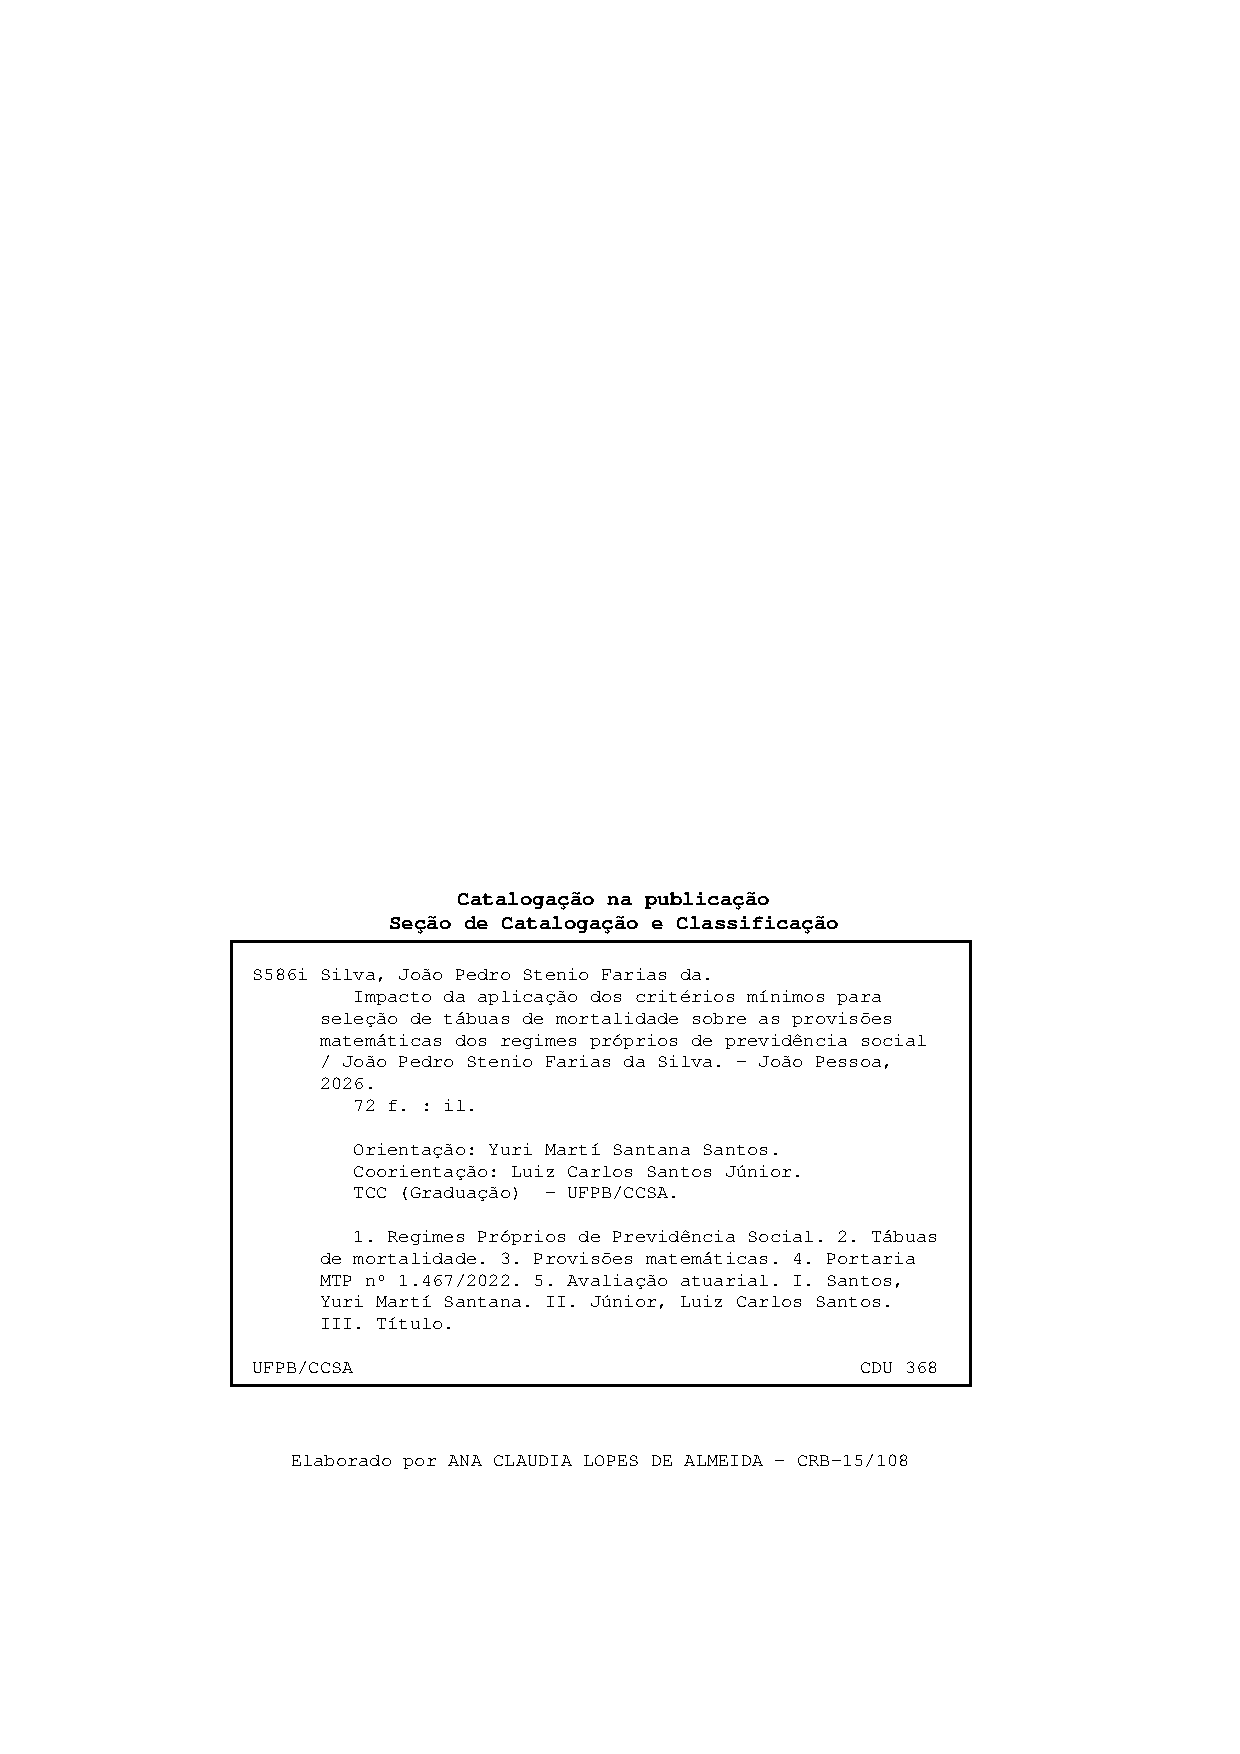
\includepdf[pages=-, fitpaper=true]{ficha_catalografica_71314.pdf}

% ===== FOLHA DE APROVAÇÃO =====
\newpage
\begin{folhadeaprovacao}
    \begin{center}
        {\normalsize\singlespacing\imprimirautor}
        \vspace*{\fill}\vspace*{\fill}
        \begin{center}
            \bfseries\normalsize\singlespacing\imprimirtitulo
        \end{center}
        \vspace*{\fill}
        
        \hspace{.45\textwidth}
        \begin{minipage}{.5\textwidth}
            \singlespacing\imprimirpreambulo
        \end{minipage}
        \vspace*{\fill}
    \end{center}
    
    \vspace{1.0cm}
    
    \begin{center}
        \textbf{BANCA EXAMINADORA}
    \end{center}
    \vspace{0.5cm}
    \assinatura{\imprimirorientador}{Orientador}{Universidade Federal da Paraíba (UFPB)}
    \vspace{0.5cm}
    \assinatura{\examinadorA}{Examinador}{Universidade Federal da Paraíba (UFPB)}
    \vspace{0.5cm}
    \assinatura{\examinadorB}{Examinadora}{Universidade Federal da Paraíba (UFPB)}
    
    
\end{folhadeaprovacao}

% ===== AGRADECIMENTOS =====
\newpage
\titulocentral{AGRADECIMENTOS}
% !TEX root = tcc.tex
\setlength{\parindent}{1.25cm}

Primeiramente, expresso minha profunda gratidão a minha família, que sempre dedicou seus esforços à minha educação. Em especial, à minha mãe Mônica, que mesmo diante das circunstâncias mais adversas jamais mediu esforços para que seus filhos pudessem seguir seus caminhos e aproveitar cada oportunidade que a vida lhes oferecia. Ao meu pai George, meu eterno agradecimento por ter sido um exemplo vivo de superação, ensinando-me, pela própria trajetória, que sou capaz de vencer qualquer obstáculo que se apresente em meu caminho. 

Ao meu amor Geovanna, agradeço pelo amor e pelo apoio incondicional em todos os momentos desta jornada. Cada dia compartilhado, cada conversa e cada risada foram fundamentais para que eu chegasse até aqui. Sem a sua presença e dedicação, esta conquista não teria o mesmo significado. 

Aos meus amigos Carlos e César, agradeço por terem compartilhado comigo a trajetória de deixar o interior de Pernambuco em busca de novos horizontes em João Pessoa. As risadas, as conversas e os momentos vividos no apartamento 303 ficarão para sempre guardados em minha memória. 

A Isaías, um verdadeiro irmão que a Universidade Federal da Paraíba me presenteou, minha mais sincera gratidão. As inúmeras tardes e noites de diálogo, nas quais compartilhávamos e debatíamos ideias que transcendiam os limites acadêmicos. 

Agradeço a todos que, de alguma forma, cruzaram meu caminho e deixaram sua marca. Em especial, a Francisca, Lucélia e a toda a equipe ADM ProKids, que me ofereceram suporte precioso no momento mais difícil da minha vida. Estendo também meu profundo agradecimento a toda a equipe de oncologia e urologia do Hospital das Clínicas da Universidade Federal de Pernambuco, cuja dedicação e humanidade tornaram cada sessão de quimioterapia mais suportável. 

Por fim, ao meu orientador Yuri e ao meu coorientador Luiz, meu mais sincero e especial agradecimento. Ambos foram pilares fundamentais na construção deste trabalho. Estendo ainda minha gratidão a todo o corpo docente com quem tive o privilégio de aprender ao longo desta trajetória.


% ===== RESUMO =====
\newpage
\titulocentral{RESUMO}
% !TEX root = tcc.tex
\begin{spacing}{1}
\noindent Os Regimes Próprios de Previdência Social (RPPS) são os sistemas responsáveis por prover benefícios pós-emprego aos servidores públicos efetivos. Nesse contexto, a Portaria MTP nº 1.467/2022 estabelece parâmetros e diretrizes para estas organizações. Em seu Art. 36, a referida Portaria estabelece como critério mínimo para a seleção de tábuas de mortalidade a exigência de que a tábua adotada apresente, na idade média da massa segurada, expectativa de vida igual ou superior à da tábua de referência (IBGE anual extrapolada por sexo). Este trabalho analisa se o critério de seleção de tábuas de mortalidade estabelecido pelo Art. 36 da referida Portaria é suficiente para garantir que a provisão matemática calculada com a tábua adotada seja igual ou superior àquela obtida com a tábua de referência. Para isso, foram realizadas simulações com quatro perfis etários distintos — jovem, equilibrado, idoso e bimodal —, cada um composto por 100.000 segurados de cada sexo, considerando um cenário simplificado com único benefício de aposentadoria por idade, salário inicial uniforme e ausência de decrementos por invalidez ou desligamento. As provisões foram calculadas pelos métodos INE, CUP e PNI, aplicando-se o critério de seleção de tábuas conforme o fluxo normativo do Art. 36. Os resultados evidenciaram inconsistências em todos os perfis etários, com maior incidência em massas jovens, especialmente para o sexo masculino. A investigação revelou que a assimetria entre os níveis de sobrevivência nas faixas contributivas (18–64 anos) e nas faixas em gozo de benefício (65 anos em diante) é o mecanismo causador. Quando a tábua comparativa projeta maior sobrevivência nas idades contributivas do que nas aposentadoras, a variação no valor das contribuições supera a variação no valor dos benefícios, resultando em provisão matemática inferior. Para auxiliar o diagnóstico prévio, propõe-se o índice $I_F$, que quantifica o diferencial de sobrevivência ponderado pela estrutura etária da massa. Conclui-se que o critério do Art. 36, ao utilizar exclusivamente a expectativa de vida na idade média como parâmetro comparativo, pode ser insuficiente para garantir que a tábua adotada produza uma provisão matemática igual ou superior à da tábua de referência em todas as configurações demográficas possíveis. 
\end{spacing}
\vspace{1.0cm}

\noindent \textbf{Palavras-chave}: Regimes Próprios de Previdência Social. Tábuas de mortalidade. Provisões matemáticas. Portaria MTP nº 1.467/2022. Avaliação atuarial.

% ===== ABSTRACT =====
\newpage
\titulocentral{ABSTRACT}
% !TEX root = tcc.tex
\begin{spacing}{1}
    \noindent The Regime Próprio de Previdência Social (RPPS) — the public sector pension  system in Brazil — is responsible for providing post-employment benefits to  permanent civil servants. In this context, Ordinance MTP No.\ 1,467/2022  establishes parameters and guidelines for these organizations. Its Article 36  sets a minimum criterion for the selection of mortality tables, requiring that  the adopted table present, at the mean age of the insured population, a life  expectancy equal to or greater than that of the reference table (the annual  IBGE table, extrapolated by sex). This study investigates whether the mortality  table selection criterion established by Article 36 is sufficient to ensure that  the mathematical provision calculated with the adopted table is equal to or  greater than that obtained with the reference table. To this end, simulations  were conducted for four distinct age profiles --- young, balanced, old, and  bimodal --- each comprising 100,000 insured individuals of each gender, under a simplified  scenario with a single old-age retirement benefit, uniform initial salary, and  no decrements due to disability or withdrawal. Mathematical provisions were  calculated using the INE, CUP, and PNI actuarial cost methods, applying the  table selection criterion in accordance with the regulatory framework of  Article 36. The results revealed inconsistencies across all age profiles, with  higher incidence in younger populations, particularly for males. The  investigation showed that the asymmetry between survival levels in the  contributory age range (18--64 years) and in the benefit-receipt age range  (65 years and older) is the underlying mechanism. When the comparative table  projects higher survival at contributory ages than at retirement ages, the  increase in the present value of contributions exceeds the increase in the  present value of benefits, yielding a mathematical provision lower than that  of the reference table. To support prior diagnosis, the index $I_F$ is  proposed, which quantifies the differential in survival rates weighted by the  age structure of the insured population. It is concluded that the criterion of  Article 36, by relying exclusively on life expectancy at the mean age as a  comparative parameter, may be insufficient to guarantee that the adopted  mortality table produces a mathematical provision equal to or greater than that  of the reference table across all possible demographic configurations.
\end{spacing}
\vspace{1.0cm}

\noindent \textbf{Keywords}: Mortality tables. Mathematical provisions. Ministerial Ordinance MTP No. 1,467/2022. Actuarial valuation.

% ===== LISTA DE QUADROS =====
%\newpage
%\listofquadros


% ===== LISTA DE TABELAS =====
\newpage

% Título customizado
\begin{center}
    \normalsize\bfseries{LISTA DE TABELAS}
\end{center}

% Usando tocloft para eliminar completamente o título e seus espaços
\renewcommand{\cftlottitlefont}{}
\renewcommand{\listtablename}{}
\setlength{\cftbeforelottitleskip}{-\baselineskip}
\setlength{\cftafterlottitleskip}{0pt}

% Adicionar "Quadro" antes do número na lista - versão alternativa
\renewcommand{\cfttabpresnum}{\bfseries{Tabela~}}
\renewcommand{\cfttabaftersnum}{~-~}
\setlength{\cfttabnumwidth}{4.75em}
\renewcommand{\cfttabdotsep}{\cftdotsep}
\vspace{0.5cm}
{\def\addvspace#1{}\listoftables}

% ===== LISTA DE FIGURAS =====
\newpage

% Título customizado
\begin{center}
    \normalsize\bfseries{LISTA DE FIGURAS}
\end{center}

% Usando tocloft para eliminar completamente o título e seus espaços
\renewcommand{\cftloftitlefont}{}
\renewcommand{\listfigurename}{}
\setlength{\cftbeforeloftitleskip}{-\baselineskip}
\setlength{\cftafterloftitleskip}{0pt}

% Adicionar "Figura" antes do número na lista
\renewcommand{\cftfigpresnum}{\bfseries{Figura~}}
\renewcommand{\cftfigaftersnum}{~-~}
\setlength{\cftfignumwidth}{4.5em}
\renewcommand{\cftfigdotsep}{\cftdotsep}
\vspace{0.5cm}
{\def\addvspace#1{}\listoffigures}


% ===== LISTA DE ABREVIATURAS E SIGLAS =====
\newpage

% Título customizado sem espaço extra
\begin{center}
    \normalsize\bfseries{LISTA DE ABREVIATURAS E SIGLAS}
\end{center}

\fontsize{12}{14}\selectfont
\begin{tabular}{ll}
BD    & Benefício Definido \\
CD    & Contribuição Definida \\
CN    & Custo Normal \\
CV    & Contribuição Variável \\
CRP   & Certificado de Regularidade Previdenciária \\
CUP   & Custo Unitário Projetado \\
IBA   & Instituto Brasileiro de Atuária \\
IBGE  & Instituto Brasileiro de Geografia e Estatística \\
INE   & Idade Normal de Entrada \\
INSS  & Instituto Nacional do Seguro Social \\
PM    & Provisão Matemática \\
PMBaC & Provisões Matemáticas de Benefícios a Conceder \\
PMBC  & Provisões Matemáticas de Benefícios Concedidos \\
PNI   & Prêmio Nivelado Individual \\
RGPS  & Regime Geral de Previdência Social \\
RPPS  & Regime Próprio de Previdência Social \\
V.A.  & Variável Aleatória \\
VABF  & Valor Atual dos Benefícios Futuros \\
VACF  & Valor Atual das Contribuições Futuras \\
\end{tabular}

% ===== SUMÁRIO =====
\newpage
\tableofcontents

% ===== INÍCIO DA PARTE TEXTUAL =====
\textual

% !TEX root = tcc.tex
\chapter{\textbf{INTRODUÇÃO}}

\section{\textbf{Contextualização e problema}}

A Constituição da República Federativa do Brasil de 1988 define, em seu Art. nº 194, o Sistema de Seguridade Social, com o objetivo de garantir direitos associados à saúde, à previdência e à assistência social. O pilar da previdência visa assegurar a renda ao trabalhador e seus dependentes em face de perda de força da capacidade laboral, invalidez ou morte \cite{brasil1988constituicao}.

O Regime Próprio de Previdência Social (RPPS), objeto do presente estudo, é o sistema previdenciário específico dos servidores públicos efetivos e tem suas normas básicas estabelecidas no Art. nº 40 da Constituição da República Federativa do Brasil \cite{brasil1988constituicao}. O Art. 1º da Lei nº 9.717/98 estabelece que os RPPS deverão ser organizados com base em normas gerais de contabilidade e atuária, de modo a garantir o seu equilíbrio financeiro e atuarial \cite{PL7776_2010}. Para que regimes de longo prazo, como os RPPS, possam honrar os compromissos futuros de seus planos previdenciários, é indispensável uma gestão financeira e de riscos rigorosa \cite{bogoni2011}. Em sua essência, como explica \citeonline{lopes2010impacto}, os planos previdenciários são mecanismos de proteção construídos para garantir recursos frente à perda de capacidade de trabalho.

O inciso I do Art. 1º da Lei nº 9.717/98 declara a obrigatoriedade da realização de avaliação atuarial inicial e em cada balanço utilizando-se parâmetros gerais, para a organização e revisão do plano de custeio e benefícios \cite{PL7776_2010}. Dentro da ciência atuarial, existe um processo que visa o gerenciamento e a avaliação de riscos e sistemas previdenciários, em geral. Esse processo é a avaliação atuarial. No contexto previdenciário, essa análise se empenha em assegurar a sustentabilidade dos planos por meio de precisas previsões sobre as obrigações futuras do plano, permitindo que os recursos auferidos sejam suficientes para cumprir essas obrigações futuras \cite{micoccini2010}.

Essa busca pela sustentabilidade ocorre por meio da verificação do equilíbrio do plano que, segundo \citeonline{correa2020premissas}, exige a comparação entre os pagamentos de benefícios e as contribuições em uma mesma data. É importante salientar que não se deve confundir o equilíbrio financeiro com o equilíbrio atuarial. A Portaria MTP nº 1.467/2022 distingue esses dois conceitos. O primeiro se refere à garantia de equivalência entre as receitas auferidas e as obrigações do RPPS em cada exercício financeiro. Já o segundo, se refere à garantia de equivalência, a valor presente, entre o fluxo das receitas estimadas e das obrigações projetadas, apuradas atuarialmente, a longo prazo \cite{mtp1467_2022}.

Como explica \citeonline{correa2020premissas}, as principais modalidades de planos são Benefício Definido (BD), cujo valor do benefício futuro é preestabelecido, e os de Contribuição Definida (CD), cujo benefício depende do saldo acumulado. Entretanto, ainda existe uma terceira modalidade, a Contribuição Variável (CV), que mescla características dos dois modelos principais. O fato de a maioria dos RPPS se enquadrar no modelo BD, cujo benefício é uma promessa futura, torna a precisão das premissas e do cálculo atuarial ainda mais crítica para a sustentabilidade do sistema \cite{correa2020premissas}.

Na análise de \citeonline{rodrigues2012risco}, as premissas atuariais devem representar a massa segurada da maneira mais coerente e realista possível. Portanto, quando estas não representam fidedignamente o grupo de segurados, isso pode gerar cálculos imprecisos, resultando em déficit ou superávit técnico. Conforme a classificação do mesmo, as premissas atuariais são divididas em três grupos: econômicas, biométricas e genéricas.

As premissas biométricas, conforme explica \citeonline{rodrigues2012risco}, representam os eventos como mortalidade, invalidez e sobrevivência. A escolha e a adequação dessas hipóteses são determinantes para a apuração fidedigna das responsabilidades do plano, influenciando diretamente o cálculo das provisões matemáticas e, por conseguinte, as alíquotas de contribuição necessárias para o financiamento dos benefícios \cite{correa2020premissas}.

Segundo dados do Ministério da Previdência Social referentes ao exercício de 2021, existiam 2.152 RPPS entre Estados, Distrito Federal e Municípios no Brasil. Desses, 1.732 estão em déficit atuarial, somando um total aproximado de R\$ 2,5 trilhões em déficit \cite{brasil_dados_rpps}.

A Portaria MTP Nº 1.467/2022 surge nesse contexto, estabelecendo parâmetros e diretrizes para as avaliações atuariais, com o objetivo de promover a higidez financeira desses regimes. Contudo, a aplicação prática das normativas pode suscitar debates sobre a adequação de determinados critérios.

A referida Portaria em sua Seção VI, Capítulo IV, estabelece critérios mínimos a partir do Art. 36, inciso I, e trata da verificação da validade das tábuas biométricas (usadas para estimar longevidade e entrada em invalidez) por meio da comparação entre expectativas de vida da seguinte forma:

\begin{citacao}
\noindent
[...] será dado pela tábua anual de mortalidade do Instituto Brasileiro de Geografia e Estatística -- IBGE, segregada obrigatoriamente por sexo, divulgada pela SPREV; e será averiguado por meio da comparação entre a Expectativa de Vida -- Ex estimada por essa tábua com aquela gerada pelas tábuas utilizadas na avaliação atuarial \cite[p.~28]{mtp1467_2022}.
\end{citacao}

Por meio desses itens, o Art. 36 da Portaria MTP nº 1.467/2022 estabelece que a tábua de mortalidade disponibilizada pelo IBGE será o mínimo aceitável. O RPPS poderá adotar outra tábua de mortalidade, desde que a expectativa de vida na idade média da massa não seja inferior à da tábua do IBGE.

A escolha da média como métrica central de avaliação convida a uma reflexão sobre a adequação desse critério avaliativo. Como explicam \citeonline{bruce2020estatistica}, a média artimética é uma medida de posição que, embora seja útil em um vasto leque de situações, acaba sendo uma medida frágil em casos com amostras assimétricas. Isso porque essa métrica é sensível a valores extremos e ignora a forma da distribuição (dispersão, assimetria e concentração). Portanto, a média artimética pode mascarar realidades demográficas quando usada para comparar populações.

A expectativa de vida, por sua vez, como explicam \citeonline{smith2001state}, é a duração média da vida futura a partir de uma idade específica, sendo obtida a partir da divisão entre o tempo total de vida restante de uma coorte e a número de pessoas vivas, o que a caracteriza, em termos matemáticos, como uma média aritmética. Consequentemente, ela sofre das limitações estatísticas inerentes a qualquer média.

A concentração de segurados em determinadas faixas etárias representa uma fragilidade atuarial com implicações financeiras significativas \cite{antolin2007longevity}. Em massas seguradas com distribuições etárias heterogêneas, indicadores baseados em médias podem mascarar riscos relevantes ao desconsiderar o comportamento da curva de mortalidade. Nesse contexto, uma tábua pode indicar maior sobrevida em idades anteriores ao ponto médio, mas apresentar menor sobrevida nas idades posteriores a esse ponto. Assim, caso haja uma concentração de segurados em faixas etárias nas quais a tábua apresenta menor sobrevida, ela poderá levar à subestimação da obrigação definida pelo limite mínimo, mesmo sendo, do ponto de vista matemático, superior no ponto médio. Dessa forma, duas carteiras com idade média similar podem apresentar riscos atuariais diferentes, dependendo de como os segurados se distribuem ao longo das faixas etárias \cite{rockefeller2016pension}.

Seja $PM^{i}$ a provisão matemática calculada a partir da tábua de mortalidade $i$. Esta grandeza é intrinsecamente dependente das anuidades atuariais e das probabilidades de sobrevivência associadas à referida tábua. A ideia de utilizar a expectativa de vida como indicador do nível da PM, produzida diferentes tábuas de mortalidade, se fundamenta no raciocínio de que segurados com maior longevidade esperada receberão benefícios por períodos mais extensos, elevando o valor presente das obrigações do plano \cite{silveira_santos_2017}.

Diante disso, formula-se a hipótese central desta pesquisa: o critério estabelecido pelo Art. 36 da Portaria MTP 1.467/2022 pressupõe, implicitamente, que uma tábua comparativa com expectativa de vida na idade média igual ou superior à da tábua de referência produzirá uma PM igual ou superior à da tábua de referência. Logo, sejam $e^{*}_{\overline{X}}$ a expectativa de vida na idade média segundo uma tábua comparativa qualquer e $PM^{*}$ a provisão matemática correspondente, sendo $e^{\kappa}_{\overline{X}}$ a expectativa de vida na idade média segundo a tábua de referência (IBGE 2024 extrapolada para cada gênero) e $PM^{\kappa}$ a respectiva provisão matemática. A hipótese pode ser expressa pela relação de ordem $e^{*}_{\overline{X}} \geq e^{\kappa}_{\overline{X}} \Rightarrow PM^{*} \geq PM^{\kappa}$. Contudo, ao simplificar tal hipótese usando a anuidade atuarial e a expectativa de vida na idade $x$, ou seja, avaliando $e^{*}_{x} \geq e^{\kappa}_{x} \Rightarrow a^{*}_{x} \geq a^{\kappa}_{x}$, é possível demonstrar que essa relação de ordem não é sempre verdadeira, como mostra o exemplo contido no \ref{apendice_A}.

Diante do exposto, e no contexto de massas seguradas com distribuições etárias assimétricas, o presente trabalho busca responder à seguinte questão central: \textbf{O critério de seleção de tábuas de mortalidade estabelecido pelo Art. 36 da Portaria MTP nº 1.467/2022 é suficiente para garantir que a provisão matemática calculada com a tábua adotada seja igual ou superior àquela obtida com a tábua de referência?}

\section{\textbf{Objetivos}}
Em razão desse cenário de desequilíbrio atuarial, marcado por cálculos que podem envolver distribuições assimétricas, apresentam-se os objetivos desta pesquisa.

\subsection{Objetivo geral}
Este estudo propõe-se a investigar se o critério de seleção de tábuas de mortalidade estabelecido pelo Art. 36 da Portaria MTP nº 1.467/2022 é suficiente para garantir que a provisão matemática calculada com a tábua adotada seja igual ou superior àquela obtida com a tábua de referência, identificando as condições demográficas e atuariais sob as quais podem ocorrer inconsistências e propondo um indicador de diagnóstico prévio.

\subsection{Objetivos específicos}

\begin{itemize}
    \item Simular cenários previdenciários segmentados em quatro perfis etários distintos para servir de base às projeções atuariais.

    \item Mensurar as provisões matemáticas para cada perfil estruturado, aplicando os métodos de custeio INE, CUP e PNI sob a ótica de diferentes tábuas de mortalidade.
    
    \item Identificar quais tábuas de mortalidade resultam em provisões matemáticas inferiores àquelas geradas pela tábua de referência, mesmo atendendo estritamente ao critério normativo vigente.
    
    \item Analisar as causas demográficas e financeiras que levam a essa subestimação.
    
    \item Propor um indicador analítico que permita sinalizar antecipadamente se uma determinada tábua tende a gerar uma provisão matemática inferior à da tábua de referência.
\end{itemize}
    
\section{\textbf{Justificativa}}

A Portaria MTP Nº 1.467/2022 surge em um contexto deficitário com a missão de estabelecer diretrizes a fim de promover o equilíbrio atuarial dos RPPS. A presente monografia se justifica pela necessidade de verificar a aplicabilidade do critério de validação de tábuas de mortalidade estabelecido no Art. 36. Essa justificativa se reforça diante da quantidade de RPPS que não utilizam as tábuas de mortalidade mínimas previstas nesse artigo. Segundo dados do Ministério da Previdência Social referentes ao exercício de 2025, aproximadamente 50\% dos RPPS não utilizaram a tábua mínima para a população masculina e a mesma proporção foi observada para a população feminina \cite{brasil_dados_rpps}.

Esta abordagem, embora intencionada a ser uma salvaguarda, simplifica a validação de um fenômeno complexo e distribucional como a mortalidade, especialmente em populações com distribuições etárias assimétricas. Tal critério ignora a dispersão e a forma da curva demográfica, que são cruciais para a correta apuração do passivo atuarial, cujo valor é diretamente impactado pela estrutura etária da carteira de segurados \cite{junior2019mortalidade}.

Uma tábua de mortalidade com expectativa de vida mais elevada, em teoria, implica em uma maior longevidade e por fim, um maior passivo atuarial \cite{silveira_santos_2017}. Estudos, como o de \citeonline{dias_santos_2009}, mostram que tábuas de mortalidade que projetam maior longevidade resultam em um valor de passivo atuarial significativamente superior. Se essa lógica é rompida, isto é, se uma tábua com maior expectativa de vida resultar em um passivo menor, isso indica uma falsa percepção de equilíbrio do RPPS, podendo comprometer a sustentabilidade do regime à longo prazo, onde futuros déficits que podem inviabilizar o pagamento de benefícios.

Ao quantificar o impacto financeiro desses possíveis cenários, esta monografia visa contribuir para a garantia dos direitos previdenciários dos servidores, sem onerar indevidamente as futuras gerações.

\section{\textbf{Estrutura do trabalho}}
Este trabalho está organizado em cinco capítulos. O primeiro introduz a pesquisa, estabelecendo o problema, os objetivos e a justificativa. O segundo capítulo dedica-se ao referencial teórico. O terceiro detalha a metodologia empregada na investigação. No quarto, são apresentados e discutidos os resultados obtidos. Finalmente, o quinto capítulo encerra o estudo com as considerações finais.

% !TEX root = tcc.tex
\chapter{\textbf{REFERENCIAL TEÓRICO}}
Este capítulo apresenta o referencial teórico do presente trabalho, um mapeamento acerca do que outros estudos investigaram quanto ao proposto pela corrente pesquisa: o impacto que a aplicação dos critérios mínimos para seleção de tábuas de mortalidade exerce sobre as provisões matemáticas. Adicionalmente, o capítulo destaca as lacunas a serem preenchidas, principalmente a ausência de estudos que validem a consistência técnica deste critério legal e quantifiquem seu potencial impacto financeiro, especialmente em cenários com distribuições etárias assimétricas. Para contextualizar a análise, são abordadas questões referentes à sustentabilidade, regulamentação, cálculo atuarial e financiamento no âmbito dos RPPS.

\section{\textbf{Sustentabilidade e regulamentação dos regimes próprios}}
O desenvolvimento sustentável do RPPS é proveniente de uma gestão coerente dos recursos, transparência e mitigação dos riscos. Sendo assim, essa sustentabilidade é instaurada como um desafio urgente para a administração pública brasileira \cite{puchalski2022}.

Para \citeonline{puchalski2022} e \citeonline{nogueira2012equilibrio}, existem diversos fatores que se destacaram na formação do desequilíbrio dos regimes de previdência dos servidores públicos. Dentre eles, houve uma expansão exponencial da criação desses regimes, sem que fossem estabelecidas as regras para a instituição. Vários regimes próprios foram instituídos como uma tentativa de aliviar temporariamente os gastos públicos, porém, sem mecanismos eficazes de controle das contribuições. Isso resultou em situações de inadimplência junto aos fundos destinados aos servidores públicos.

A compreensão do que são o equilíbrio financeiro e o equilíbrio atuarial foi estabelecida na Emenda Constitucional nº 20/1998. Esse entendimento é exposto no Art. nº 40 da Constituição Federal, ao propagar que o regime de previdência dos servidores públicos deverá observar critérios que preservem o equilíbrio financeiro e atuarial, sendo esses os princípios básicos que guiam a existência desses regimes \cite{puchalski2022, nogueira2012equilibrio}.

Entretanto, foi somente com a Lei nº 9.717, de 27 de novembro de 1998, que a definição se tornou mais específica, estabelecendo normas gerais de contabilidade e atuária como parâmetros a serem examinados para a organização dos regimes próprios, com o objetivo de assegurar o equilíbrio financeiro e atuarial. A partir do Decreto nº 3.788/2001, esses critérios passaram a ser exigidos nos regimes próprios, para que pudessem comprovar a regularidade de seus RPPS perante a Secretaria de Previdência Social e, assim, obter o Certificado de Regularidade Previdenciária (CRP) \cite{puchalski2022}.

A Portaria MTP Nº 1.467, de 2 de junho de 2022, surge em um contexto de desequilíbrio atuarial, com o objetivo de estabelecer um marco regulatório robusto para os RPPS da União, dos Estados, do Distrito Federal e dos Municípios. A Portaria define diretrizes essenciais para a organização e operação desses regimes, abordando diversos aspectos das avaliações atuariais \cite{silva2024sustentabilidade}. Ela estabelece em sua seção VI, entre outros, parâmetros mínimos de prudência para a escolha das hipóteses atuariais, buscando garantir a sustentabilidade e a eficiência financeira dos RPPS.

O foco do presente trabalho se restringe ao Art. 36, inciso I, da referida Portaria. O texto normativo estabelece os critérios para a utilização de tábuas biométricas a serem utilizadas nos cálculos atuariais. Além das alíneas 'a' e 'b', citadas no primeiro capítulo, a norma estabelece em seu parágrafo único que a o RPPS poderá utilizar tábuas biométricas elaboradas a partir da experiência da massa segurada, desde que atendidos os limites minímos deste mesmo artigo.

Ao estabelecer um \textit{benchmark} mínimo de longevidade, busca-se mitigar o risco de que os RPPS utilizem tábuas de mortalidade que subestimem a sobrevida dos seus participantes e, consequentemente, levem a uma subestimação do passivo atuarial. A tábua de mortalidade do IBGE, por representar a população geral, é posicionada como um limite de segurança.

\section{\textbf{Cálculo atuarial em sistemas previdenciários}}

Para entidades que geram passivos de longo prazo, como os RPPS, um aspecto relevante é a incerteza sobre quanto tempo as pessoas vão viver. O risco de longevidade representa a sobrevivência das pessoas a mais do esperado. A natureza persistente e sistemática do risco de longevidade, em particular, exige que os entes busquem formas robustas de sustentabilidade \cite{bravo2007}.

O cálculo atuarial nos RPPS fundamenta-se na aplicação de técnicas biométricas e financeiras para lidar com o risco de longevidade e assim estimar as contribuições devidas pelos participantes e os benefícios a serem pagos pela entidade gestora \cite{lopes2010impacto}. Conforme explicam \citeonline{rodrigues2012risco} e \citeonline{correa2020premissas}, essa metodologia combina o uso de tábuas de mortalidade com técnicas de desconto financeiro para projetar os fluxos de caixa previdenciários ao longo do tempo.

Neste sentido, este tópico apresenta informações sobre as técnicas financeiras, com base em funções de desconto de um ou mais pagamentos, bem como sobre as técnicas biométricas, a partir das tábuas de mortalidade, e as obrigações da entidade gestora relacionadas à formação das provisões matemáticas.

\subsection{Desconto de um ou mais pagamentos}

Todo e qualquer contrato que lide com conceitos financeiros exige considerar o valor do dinheiro no tempo. A matemática financeira mostra que é possível realizar tal avaliação através da taxa de juros. Portanto, através da equação \ref{eq:v}, é possível obter o valor presente de alguma quantia monetária futura \cite{rodrigues2012risco}.

\begin{equation}
    v = \left(\frac{1}{1+i}\right)^{n}
    \label{eq:v}
\end{equation}

\noindent Em que $i$ representa a taxa de juros e $n$ o prazo associado à quantia monetária futura. Uma renda é uma série de pagamentos e podem ser certas ou aleatórias. As rendas certas são tratadas pelas matemática financeira. Já as rendas aleatórias, são o foco na matemática atuarial \cite{cordeiro2014calculo, vilanoca1969}.

Na renda certa, a duração e o fluxo de pagamentos são determinados por um prazo fixo, independentemente de quem está recebendo ou pagando estar vivo ou não, como mostra a equação \ref{eq:an} \cite{rodrigues2012risco}.

\begin{equation}
    \ddot{a}_{n} = \sum_{t=0}^{n} \left(\frac{1}{1+i}\right)^{t}
    \label{eq:an}
\end{equation}

Já nas rendas aleatórias, os pagamentos estão diretamente vinculados à vida futura de um participante de idade $x$. Ou seja, os valores só serão pagos enquanto a pessoa estiver viva, de acordo com a equação \ref{eq:ax} \cite{bowers2006}.

\begin{equation}
    \ddot{a}_{x} = \sum_{t=0}^{\infty} \left(\frac{1}{1+i}\right)^t \cdot {}_{t}p_{x}
    \label{eq:ax}
\end{equation}

Portanto, a principal diferença entre essas duas rendas está na duração do pagamento: na renda certa, a duração é predeterminada por um prazo fixo, cessando os pagamentos ao final desse período, independentemente das circunstâncias. Já na renda aleatória, a duração é incerta, pois está condicionada à sobrevivência de uma ou mais pessoas. Os pagamentos, neste caso, persistem enquanto o indivíduo estiver vivo, podendo se estender por toda a sua vida ou por um período pré-definido, desde que a condição de sobrevivência seja atendida \cite{vilanoca1969}.

\subsection{Tábuas de mortalidade}

A tábua de mortalidade descreve o padrão de mortalidade observado em uma população específica. Em sua forma clássica demográfica, ela se dispõe como uma tabela que possui informações sobre como uma coorte de nascimentos vai, ao longo do tempo, extinguindo-se. Uma de suas colunas é dedicada à idade. As demais colunas são preenchidas com funções relacionadas à mortalidade, específicas para cada idade \cite{preston2001demography}. 

A visão da ciência atuarial dessa ferramenta não se obstem muito desta que foi apresentada. De acordo com \citeonline{cordeiro2014calculo}, uma tábua de mortalidade é um recurso que permite entender a mortalidade de um determinado grupo. É, dessa forma, um instrumento estatístico com o objetivo de mensurar, por idade, probabilidades referentes à vida e morte das pessoas. Para cada idade, nestes casos, são apresentadas as quantidades de falecimentos, a taxa de mortalidade específica, a probabilidade de falecimentos, a probabilidade de sobrevivência e a esperança de vida. Como explica \citeonline{paes2018}, a tábua de mortalidade possui grande relevância prática para as ciências atuariais, uma vez que essa área utiliza as probabilidades nela contidas para a realização de cálculos nos setores de seguros e previdência.

\subsubsection{\textit{Tempo residual de vida e funções biométricas decorrentes}}

Nos cálculos atuariais do ramo vida representamos a variável aleatória (V.A.) contínua "tempo futuro de vida"{} pela notação $T_x$ \cite{bowers2006, dickson2019, macdonald2018}. Atuários se utilizam dessa variável como base para o desenvolvimento de tábuas de mortalidade, de forma que possam avaliar a mortalidade e a longevidade de um grupo, devido a esses serem parâmetros essenciais para os cálculos de benefícios no ramo vida \cite{dickson2019,promislow2015}.

Seja $F_x(t)$ a função de distribuição acumulada associada a V.A. tempo futuro de vida ($T_x$), conforme expressa a equação \ref{eq:Fx}. Assim, $F_x(t)$ representa a probabilidade de que uma pessoa de idade exata $x$ morra em até $t$ anos.

\begin{equation}
    F_x (t)= P(T_x \leq t), \quad \forall x > 0
    \label{eq:Fx}
\end{equation}

A função de densidade $f_x(t)$ é obtida através da derivação de $F_x(t)$, como mostra \ref{eq:fx}. Essa função descreve a probabilidade de uma pessoa falecer em um instante $t$.

\begin{equation}
    f_x (t)= \frac{d}{dt}[F_x(t)], \quad \forall x > 0
    \label{eq:fx}
\end{equation}

Por vezes, atuários estão interessados em entender a probabilidade de que uma pessoa com idade exata $x$ sobreviva por pelo menos $t$ anos. Essa probabilidade é denominada como função de sobrevivência $S_x(t)$, expressada em \ref{eq:Sx}.

\begin{equation}
    S_x (t)= P(T_x>t)=1-F_x(t), \quad \forall x > 0
    \label{eq:Sx}
\end{equation}

Como explicam \citeonline{macdonald2018}, a notação atuarial internacional utiliza as funções $S_x(t)$ e $F_x(t)$ para representar, respectivamente, as funções biométricas ${}_tp_x$ e ${}_tq_x$, que indicam a probabilidade de sobrevivência e de morte entre as idades $x$ e $x + t$, como mostram as equações \ref{eq:sxpx} e \ref{eq:fxqx}.
\begin{equation}
    S_x(t) = {}_tp_x
    \label{eq:sxpx}
\end{equation}
\begin{equation}
    F_x(t) = {}_tq_x
    \label{eq:fxqx}
\end{equation}

As equações expostas em \ref{eq:sxpx} e \ref{eq:fxqx} possuem uma relação. Como são eventos complementares, a soma de suas probabilidades devem "cobrir" \hspace{0.025cm} todos os eventos possíveis \cite{dickson2019}, como mostra a equação \ref{eq:1pq}.
\begin{equation}
    p_x+q_x=1
    \label{eq:1pq}
\end{equation}

De acordo com \citeonline{dickson2019}, qualquer função de sobrevivência para a distribuição do tempo futuro de vida deve satisfazer as seguintes condições para ser válida: a probabilidade para um indivíduo de idade $x$ sobreviver 0 ano é 100\%; e para $t \to \infty$, todos indivíduos eventualmente irão morrer.

Além dessas, \citeonline{garcEsimoes2010} explicam que existe mais uma condição a ser satisfeita: a função é decrescente, ou seja, a primeira derivada da função de sobrevivência é negativa.

A força de mortalidade é uma função que oferece uma compreensão numérica acerca do risco de uma pessoa falecer em um curto intervalo de tempo. Especificamente, para intervalos infinitesimais de $\Delta x$. Denotada por $\mu_x$, é uma peça chave na modelagem atuarial, especialmente ao considerar o risco de mortalidade para uma pessoa viva na idade $x$ \cite{dickson2019, macdonald2018}. Essa função pode ser expressa a partir de uma relação com as equações \ref{eq:fx}  e \ref{eq:Sx}, como mostra \ref{eq:mux}.

\begin{equation}
    \mu_{x+t} = \frac{f_x(t)}{S_x(t)}
    \label{eq:mux}
\end{equation}

Existem outras duas funções biométricas básicas em uma tábua de mortalidade. São elas: o número de sobreviventes à idade $x$ e o o número de mortos entre as idades $x$ e $x+1$, denotadas por $l_x$ e $d_x$ respectivamente \cite{bowers2006}. Podemos encontrar essa duas funções utilizando a função de sobrevivência (equação \ref{eq:sxpx}) em termos apenas da força de mortalidade, como mostra  a equação \ref{eq:sxmu} e demonstrado no apêndice (equação \ref{eq:A-sxmu}).
\begin{equation}
    {}_tp_x=S_x(t)=e^{-\int_0^t\mu_{x+u}du} 
    \label{eq:sxmu}
\end{equation}

Em mãos de \ref{eq:sxmu}, é possível encontrar a função biométrica $l_x$, conforme \ref{eq:lx}. Para a determinação da coorte hipotética, escolhe-se um número arbitrário para $l_0$ (o número de pessoas vivas à idade exata 0), por exemplo, $100.000$, o que permite calcular, a partir da equação \ref{eq:lx}, o número de vivos para todas as idades. Conhecer o vetor $l_x$ viabiliza o cálculo da função biométrica $d_x$, representado pela expressão \ref{eq:dx} \cite{bowers2006, macdonald2018}. Existem outras formas de se obter os valores de $l_x$ e $d_x$, como as expostas em \citeonline{dickson2019} e \citeonline{promislow2015}, por exemplo.
\begin{equation}
    l_x=l_0\cdot S_x(t)=l_0 \cdot e^{-\int_0^t\mu_{x+u}du}
    \label{eq:lx}
\end{equation}
\begin{equation}
    {}_td_x=l_x-l_{x+t}
    \label{eq:dx}
\end{equation}

Existe uma função biométrica na tábua de mortalidade que informa o valor esperado da V.A. $T_x$, isto é, $E[T_x]$. A notação atuarial para essa função é $e_x^0$, usualmente chamada de expectativa de vida abreviada à idade $x$. A ideia fundamental é que a expectativa de vida é o tempo médio residual de vida \cite{promislow2015}. Como mostra o detalhamento no \ref{apendice_B}, é possível obter o valor de $e_x^0$ a partir da definição da esperança matemática de uma variável aleatória.

\begin{equation}
    e_x^0=E[T_x]=\int_0^\infty {}_tp_xdt
    \label{eq:ex}
\end{equation}

Embora a idade seja o principal fator, não é o único parâmetro que determina a mortalidade de uma pessoa. Fatores como gênero, estado de saúde, estilo de vida e localização geográfica também afetam a expectativa de vida. Selecionar a tábua de mortalidade apropriada para cada situação é uma tarefa crucial para um atuário \cite{promislow2015}.

\subsubsection{\textit{Classificação das tábuas de mortalidade}}

Na visão de \citeonline{bravo2007}, as tábuas de mortalidade constituem uma representação estatística do comportamento da mortalidade em uma determinada população, e a forma como são construídas ou o que elas representam define seus tipos. Elas podem ser classificadas, quanto ao tempo de observação da mortalidade, em tábuas contemporâneas e tábuas geracionais \cite{bravo2007, ortega1987}.

As tábuas contemporâneas baseiam-se na análise de uma população em um dado período, considerando as condições de mortalidade observadas naquele momento. Trata-se da aplicação das taxas de mortalidade registradas nesse intervalo temporal a uma população hipotética, usualmente composta por 100.000 indivíduos \cite{bravo2007, ortega1987}.

As tábuas geracionais, ao contrário das contemporâneas, nos permitem acompanhar um grupo de pessoas desde o seu nascimento até a morte. Estas tábuas calculam as taxas de mortalidade para a mesma geração, acompanhando a vida dos indivíduos ao longo do tempo \cite{bravo2007, ortega1987}.

Além dessas duas categorias, as tábuas também podem ser classificadas de acordo com a variação da mortalidade observada ao longo do tempo. Sob esse critério, existem as tábuas estáticas e as tábuas dinâmicas. A primeira é considerada mais simples; todas as funções de mortalidade se referem apenas à idade $x$. Elas não incorporam uma dimensão de tempo cronológico futuro. Por sua vez, a segunda classificação é mais complexa e bidimensional. Essa tábuas levam em conta não só a idade, mas também o ano de calendário (tempo cronológico). Isso permite que elas projetem a mortalidade no futuro, considerando que as taxas de morte podem mudar ao longo do tempo. São essenciais para prever como a mortalidade evoluirá \cite{bravo2007}.

Segundo \citeonline{paes2018}, as tábuas de mortalidade também podem ser classificadas em tábuas completas e tábuas abreviadas. As primeiras trabalham com a idade anual dos indivíduos, enquanto as segundas utilizam faixas etárias agregadas de cinco em cinco anos, com exceção dos grupos de 0 a 1 e de 1 a 4 anos, bem como do último intervalo, que é aberto (por exemplo, 80 anos ou mais).

\subsection{Provisões matemáticas}
A provisão matemática (PM) é utilizada pela matemática atuarial para ir de encontro ao equilíbrio atuarial. Nesse contexto, é a quantidade monetária que o ente deve ter no tempo $t$ para arcar com suas obrigações futuras \cite{cordeiro2014calculo, vilanoca1969}.

Denominada por ${}_tV$, para obter tal mensuração, existem duas metodologias principais, chamadas de métodos prospectivo e retrospectivo \cite{cordeiro2014calculo, vilanoca1969, dickson2019}. Para o método prospectivo, o ente calcula a reserva olhando para todas as obrigações e recebimentos futuros relacionados aquele grupo de segurados, como mostra \ref{eq:vtp}. Já o método retrospectivo, por sua vez, faz o inverso. Isto é, leva em consideração os prêmios que já foram pagos e os compromissos que o ente já teve até o momento da avaliação, como mostra \ref{eq:vtr} \cite{bowers2006, jordan2003}.
\begin{equation}
    {}_tV=VPA(\text{‘‘Obrigações do ente’’})-VPA(\text{‘‘Prêmios futuros’’})
    \label{eq:vtp}
\end{equation}
\begin{equation} 
    {}_tV=VA(\text{‘‘Prêmio recebidos’’})-VA(\text{‘‘Benefícios cedidos’’})
    \label{eq:vtr} 
\end{equation}

Em um contexto previdenciário, o cálculo da PM tem como objetivo cobrir as obrigações futuras do ente frente aos seus segurados, sendo esta dividida em benefícios concedidos e benefícios a conceder \cite{chan2010, rodrigues2012risco}. Dessa forma, a PM geral é dividida em Provisões Matemáticas de Benefícios Concedidos (PMBC) e as Provisões Matemáticas de Benefícios a Conceder (PMBaC), como mostra a equação \ref{eq:pm_tot} \cite{rodrigues2012risco}.
\begin{equation} 
    PM_{total} = PMBC_{total} + PMBaC_{total}
    \label{eq:pm_tot} 
\end{equation}

A distinção entre essas provisões reside na fase em que se encontram os beneficiários. A PMBC é constituída a partir do momento em que o segurado começa a usufruir dos benefícios. Neste ponto, espera-se que o plano tenha arrecadado toda a contribuição necessária do segurado e, portanto, a PMBC corresponde ao valor dos recursos garantidores necessários para o pagamento dos benefícios já em curso. Isto é, a PMBC equivale apenas ao Valor Atual dos Benefícios Futuros (VABF), devido à inexistência de novas contribuições. Nesse contexto, a equação \ref{eq:vtp} pode ser reescrita como \ref{eq:pmbc} \cite{rodrigues2012risco, gushiken2003rpps}.

\begin{equation} 
    PMBC_{total} = FCS \cdot 13 \cdot \Sigma [VABF^{i}_{Inativo}]
    \label{eq:pmbc} 
\end{equation}

\noindent Onde $FCS$ representa o fator de capacidade salarial. Entretanto, o Art. 40 da Emenda Constitucional nº 41, de 19 de dezembro de 2003, em seu § 18 estabelece que será cobrado contribuição sobre os benecífios de aposentadorias e pensões outorgadas pelo RPPS que superem o limite máximo estabelecido para os benefícios do RGPS, aplicando-se a mesma alíquota dos servidores titulares de cargos efetivos. Nesse contexto, a equação da PMBC é a diferença entra o VABF e o Valor Atual das Contribuições Futuras (VACF) e pode ser obtida por \ref{eq:pmbcteto}.
\begin{equation} 
    PMBC = FCS \cdot 13 \cdot \Sigma [VABF_{Inativo}^{i} - VACF_{Inativo}^{i}]
    \label{eq:pmbcteto} 
\end{equation}

\noindent O VABF utilizado tanto na equação \ref{eq:pmbc} quanto na equação \ref{eq:pmbcteto} pode ser obtido conforme \ref{eq:vabfpmbc} \cite{winklevoos1993}. Já o VACF usado na equação \ref{eq:pmbcteto} é cálculado usando a equação \ref{eq:vacfpmbc} \cite{rodrigues2012risco}, em que $B_r$ representa o benefício acumulado na idade $r$, ${}^{(\%)}CN$ representa o Custo Normal (CN) do plano e $\ddot{a}_x$ o fator de desconto atuarial na idade $x$.

\begin{equation} 
    VABF_{Inativo} = B_r \cdot \ddot{a}_x
    \label{eq:vabfpmbc} 
\end{equation}
\begin{equation} 
    VACF_{Inativo} = B_r \cdot \ddot{a}_x \cdot {}^{(\%)}CN
    \label{eq:vacfpmbc} 
\end{equation}

Já a PMBaC, por sua vez, situa-se na fase de contribuição. Ou seja, refere-se aos benefícios que ainda serão concedidos no futuro. É calculada como a diferença entre as obrigações futuras do ente e a arrecadação das contribuições futuras. Portanto, nesse contexto, \ref{eq:vtp} se torna \ref{eq:pmbac}. Isto é, a PMBaC é a diferença entre VABF e VACF \cite{rodrigues2012risco}.
\begin{equation} 
    PMBaC_{total} = FCS \cdot 13 \cdot \Sigma [VABF_{Ativo}^{i} - VACF_{Ativo}^{i}]
    \label{eq:pmbac} 
\end{equation}

A forma básica para o VABF de um segurado pode ser obtido conforme a equação \ref{eq:VABF}, conforme exposto em \citeonline{winklevoos1993}. O VACF, por sua vez, também pode ser encontrado em sua forma básica a partir da equação \ref{eq:VACF} \cite{rodrigues2012risco}.
\begin{equation}
    VABF_{Ativo} = B_r \cdot {}_{r-x}E_x \cdot \ddot{a}_r
    \label{eq:VABF}
\end{equation}
\begin{equation}
    VACF_{Ativo} = S_x \cdot {}^{(\%)}CN\cdot {}^{s}\ddot{a}_{x:r-x}
    \label{eq:VACF}
\end{equation}

Onde $S_x$ representa o salário do participante na idade $x$, ${}^{s}\ddot{a}_{x:r-x}$ é fator de desconto atuarial temporário na idade $x$ com crescimento salarial, $r$ a idade de aposentadoria e ${}^{(\%)}CN$ representa CN do plano. O CN de um plano de previdência é definido como o valor das necessidades de custeio mensal calculadas atuarialmente. Em termos simples, é a contribuição suficiente para manter um fundo previdenciário em equilíbrio \cite{correa2020premissas}.

\section{\textbf{Financiamento dos regimes próprios}}

Para cumprir seus objetivos, um sistema previdenciário busca a gestão eficiente de seus recursos. Para tal, se espera que este seja financiável, sustentável e capaz de suportar oscilações econômicas, demográficas e políticas. Esses sistemas previdenciários são formados sob um regime financeiro (além de um método de custeio, no caso da capitalização) e uma modalidade \cite{feldstein2001}.

No contexto de RPPS, devido ao benefício ser estabelecido na Constituição Federal, entende-se que essas entidades operem na modalidade de benefício definido.  Nesse sentido não há o que se falar em modalidades de planos em RPPS \cite{correa2020premissas}. No modelo BD, o participante sabe previamente o valor do benefício que receberá na sua aposentadoria, ou seja, o benefício é pré-determinado ou segue fórmulas estipuladas no regulamento. Os valores das contribuições, tanto do participante quanto do patrocinador, são calculados atuarialmente e podem variar ao longo do tempo para garantir o pagamento do benefício definido \cite{pinheiro2007}.

\subsection{Regimes financeiros}

Os regimes de financiamento são mecanismos que determinam como os recursos são arrecadados e utilizados para garantir o cumprimento das obrigações de aposentadorias e pensões \cite{correa2020premissas, pinheiro2007}. De acordo com o Art. 30 da Portaria 1.467/2022, os entes federativos poderão adotar, para apuração dos compromissos e determinação dos custos do plano de benefícios do RPPS, os seguintes regimes: a repartição de capitais por cobertura; e a capitalização.

O regime de capitalização é baseado em poupança, constituindo dessa forma, uma provisão matemática ao longo da vida laboral do segurado. As contribuições são investidas em ativos financeiros com a premissa que as reservas financeiras formadas sejam suficientes para cobrir os compromissos futuros \cite{pinheiro2007}. O Art. 30 da referida Portaria, determina que o regime de capitalização deve ser usado para o cálculo dos compromissos futuros relativos às aposentadorias programadas e pensões por morte decorrentes dessas aposentadorias.

O regime de capital de cobertura é uma combinação dos regimes de repartição e capitalização. Nesse regime a constituição da provisão acontece no momento de início de benefício \cite{pinheiro2007}. Este regime, como explica o Art. 30 da Portaria 1.467/2022, pode ser usado como o mínimo aplicável para cálculo envolvendo benefícios não programáveis, tais como: aposentadorias por invalidez, pensões por morte delas decorrentes e pensões por morte de segurados em atividade. 

\subsection{Métodos de custeio}

A forma como as contribuições são calculadas varia de acordo com o método de custeio adotado. Os métodos de custeio são as ferramentas utilizadas pelo atuário para estabelecer o nível de constituição das provisões necessárias para cobrir os benefícios \cite{correa2020premissas, pinheiro2007}. Segundo o Art. 31. da Portaria MTP nº 1.467/2022, deverá ser utilizado, para apuração do custo normal dos benefícios avaliados, um dos seguintes métodos de custeio: I - Crédito Unitário Projetado (CUP); II - Idade Normal de Entrada (INE);  III - Prêmio Nivelado Individual (PNI); IV - Agregado ou Ortodoxo.

O CUP é método de custeio que possui a menor complexibilidade dentre os discutidos nessa subseção \cite{almeidavieira2024}. O CN é calculado com base em frações anuais projetadas desde a idade de início da contribuição do segurado até a idade estimada de aposentadoria. Além disso, as contribuições são individuais e tendem a ser crescentes ao longo da fase contributiva \cite{winklevoos1993}. Sendo assim, o valor das obrigações futuras do plano é capitalizado de maneira uniforme entre a idade de entrada $y$ e a idade de aposentadoria $r$ \cite{winklevoos1993}. Portanto, o CN por esse método é simplesmente o $VABF_x$ dividido pelo tempo total de contribuição, conforme mostra a equação \ref{eq:CN_cup} \cite{winklevoos1993, almeidavieira2024}. 
\begin{equation}
    CN_{CUP} = \frac{VABF^{i}_{x}}{r-y}
    \label{eq:CN_cup}
\end{equation}

Consequentemente, para a apuração da PM nesse método é necessário observar da ausência das rendas aleatórias no cálculo do CN. Portanto, as contribuições futuras devem ser calculadas pelo produto entre o $CN_i$ e o tempo futuro de serviço, segundo a equação \ref{eq:VACF_cup} \cite{almeidavieira2024}.
\begin{equation}
    VACF_{CUP} = \frac{VABF^{i}_{x}}{r-y} \cdot (r - x)
    \label{eq:VACF_cup}
\end{equation}


No método INE, o CN é mais constante ao longo do tempo. A contribuição é calculada uniformemente desde a data de admissão do participante, de modo que o VABF seja amortizado ao longo do período até a data de início do benefício \cite{winklevoos1993, andreson1992}. Este método é utilizado por muitos RPPS por apresentar um custo normal estável e ser mais robusto em relação ao envelhecimento populacional e à proximidade da aposentadoria, diferentemente do CUP, visto anteriormente \cite{almeidavieira2024}.

Esse método pode ser expresso, segundo \citeonline{winklevoos1993}, como um valor fixo ao longo da vida laboral ou como uma porcentagem constante do salário do empregado. A fórmula do custo normal utilizada no presente trabalho para esse método de custeio é apresentada na equação \ref{eq:CN_ien}. Em decorrência dessa metodologia de cálculo do $CN_{INE}$, o $VACF_{INE}$ é calculado de acordo com a equação \ref{eq:VACF_ein}, conforme exposto por \citeonline{winklevoos1993}.
\begin{equation}
    CN_{INE} = \frac{VABF^{i}_{y}}{\ddot{a}_{y:r-y}}
    \label{eq:CN_ien}
\end{equation}
\begin{equation}
    VACF^{INE}_{x} = \frac{VABF^{i}_{y}}{\ddot{a}_{y:r-y}} \cdot \ddot{a}_{x:r-x}
    \label{eq:VACF_ein}
\end{equation}

No método de custeio Prêmio Nivelado Individual (PNI), por sua vez, as contribuições são uniformizadas ao longo da fase contributiva. O CN nesse método tende a aumentar ao longo dos anos, sendo inferior no início, quando comparado ao método PUC, o que resulta em um crescimento exponencial da reserva garantidora \cite{almeidavieira2024}. A forma de obter o CN por esse método de custeio consiste em apurar uma Aliquota de Custo Normal (ACN) conforme a equação \ref{eq:ACN_pni}.
\begin{equation}
    ACN^{\%}_{i} = \frac{VABF^{i}_{y}}{VASF^{i}_{y}}
    \label{eq:ACN_pni}
\end{equation}

Para calcular o $VACF_x$ nesse método de custeio, posterior ao cálculo de \ref{eq:ACN_pni}, é necessário também calcular o Valor Atual dos Salários Futuros (VASF), de acordo com a fórmula \ref{eq:VASF}. Portanto, o $VACF_x$ se dá pelo produto das equações \ref{eq:ACN_pni} e \ref{eq:VASF}, como exposto na equação \ref{eq:VACF_pni} \cite{almeidavieira2024}.
\begin{equation}
    VASF_{PNI} = \sum_{t=0}^{r-x-1} S_x\cdot(1+is)^{t} \cdot {}_{t}p_{x} \cdot v^{t}
    \label{eq:VASF}
\end{equation}
\begin{equation}
    VACF_{PNI} = ACN^{\%}_{i} \cdot VASF_{PNI}
    \label{eq:VACF_pni}
\end{equation}

O método Agregado, diferente dos métodos individuais, consiste em financiar todo o passivo atuarial inicial e quaisquer ganhos e perdas atuariais que ocorram de forma prospectiva, ao longo do tempo de serviço restante até a aposentadoria. As contribuições são coletivas e podem ser constantes ou crescentes \cite{andreson1992}.

Como explicam \citeonline{almeidavieira2024}, no método Agregado, essencialmente, não há apuração de desequilíbrios técnico-atuariais, uma vez que as alíquotas a serem aplicadas imediatamente após a avaliação atuarial são determinadas considerando-se a parcela do VABF ainda não coberta pelo patrimônio garantidor. Dessa forma, obtém-se, de maneira efetiva, uma alíquota de equilíbrio para a massa de segurados, tendo como referência o VASF conforme a equação \ref{eq:agg}.
\begin{equation}
    AE^{\%} = \frac{\Sigma VABF_i - PCP}{\Sigma VASF_i}
    \label{eq:agg}
\end{equation}

\noindent Onde $PCP$ corresponde ao Patrimônio de Cobertura do Plano, ou seja, o ativo liquido reservado para o pagamento dos benefícios futuros. Dessa forma, com a equação \ref{eq:agg} é possível aplicar essa alíquota de equilíbrio sobre a $VASF$, como mostra a equação \ref{eq:vacf_agg}, e encontrar o $VACF$ nesse método de custeio \cite{almeidavieira2024}.
\begin{equation}
    VACF = AE^{\%} \cdot VASF
    \label{eq:vacf_agg}
\end{equation}

\section{\textbf{Revisão da literatura}}

Embora não tenham sido identificados estudos que explorem especificamente aspectos legais ou testem a aplicabilidade da legislação previdenciária no contexto dos cálculos atuariais, a literatura acadêmica apresenta contribuições significativas que convergem com a problemática desta pesquisa. Os trabalhos de \citeonline{castro2019, gonzaga2022, rocha2024} abordam principalmente aspectos técnicos relacionados aos riscos demográficos e à adequação das ferramentas atuariais utilizadas nos sistemas previdenciários brasileiros, fornecendo subsídios teóricos que fundamentam a análise proposta neste estudo.

A pesquisa de \citeonline{castro2019} oferece um panorama essencial sobre a evolução da mortalidade no Brasil e o crescente risco de longevidade. O autor ressalta que as projeções da mortalidade são cruciais para estimar a expectativa de sobrevivência e subsidiar decisões governamentais sobre alocação de recursos e planejamento de políticas sociais e econômicas. Segundo \citeonline{castro2019} as tábuas de mortalidade estáticas, ao ignorarem o ganho de sobrevida, subestimam significativamente as responsabilidades atuariais das instituições previdenciárias. Para contornar essa falha, o trabalho de \citeonline{castro2019} propõe a construção de uma "Tábua BR-Geracional", que incorpora a perspectiva de sobrevivência futura de coorte, permitindo a quantificação do impacto do risco de longevidade nos diversos segmentos previdenciários brasileiros. Ele conclui que o risco de longevidade deve ser obrigatoriamente considerado no novo arcabouço legal.

O estudo de \citeonline{gonzaga2022} aprofunda a análise dos diferenciais de mortalidade entre distintos grupos de beneficiários do Instituto Nacional do Seguro Social (INSS) no Brasil. Essa pesquisa demonstra que a mortalidade não é uniforme em toda a população. Por exemplo, os aposentados por idade urbana, rural e por tempo de contribuição geralmente vivem mais do que a média nacional, enquanto os beneficiários de amparos assistenciais apresentam maiores taxas de mortalidade. Essa constatação implica que a utilização de uma tábua de mortalidade genérica ou de critérios mínimos que não considerem a heterogeneidade da população segurada pode levar a cálculos atuariais imprecisos e a desequilíbrios financeiros e atuariais do sistema. O trabalho reforça a necessidade de estudos aprofundados sobre esses diferenciais para a correta avaliação do equilíbrio financeiro e atuarial.

A importância de tábuas de mortalidade personalizadas é ainda mais salientada por \citeonline{rocha2024}, que se debruçaram sobre a mortalidade dos servidores públicos do RPPS do estado do Ceará. Este estudo demonstrou concretamente que a esperança de vida dos servidores públicos é significativamente mais elevada do que a da população nacional, com uma diferença superior a 10\% aos 60 anos de idade. Consequentemente, a adoção de tábuas de mortalidade baseadas na experiência da população geral brasileira pode subestimar as obrigações atuariais do RPPS. \citeonline{rocha2024} concluem que as tábuas de mortalidade específicas, elaboradas a partir da experiência do próprio grupo segurado, são mais eficazes e se ajustam melhor à realidade do regime de previdência, em comparação com tábuas nacionais ou internacionais comumente empregadas.

Com base na fundamentação teórica apresentada, que detalhou os conceitos de sustentabilidade, o arcabouço regulatório dos RPPS, os princípios do cálculo atuarial dos métodos de financiamento, torna-se evidente a complexidade envolvida na gestão desses regimes. A análise da literatura expôs a criticidade da escolha das premissas atuariais, em especial as tábuas de mortalidade, e as lacunas existentes no que tange à validação de critérios normativos como o estabelecido no Art. 36 da Portaria MTP Nº 1.467/2022. Tendo estabelecido este referencial, o capítulo seguinte detalhará a metodologia empregada para investigar empiricamente o impacto deste critério sobre as provisões matemáticas, utilizando uma base de dados simulados.

% !TEX root = tcc.tex
\chapter{\textbf{METODOLOGIA}}
Esta seção descreve os métodos utilizados para investigar a questão central da pesquisa: qual é o impacto da aplicação dos critérios mínimos para a seleção de tábuas de mortalidade, conforme o Art. 36, inciso I, da Seção VI, Capítulo IV, da Portaria MTP nº 1.467/2022, sobre as provisões matemáticas. São apresentados os tipos de pesquisa empregados, as bases de dados utilizadas e os procedimentos de tratamento adotados. Em seguida, expõem-se os critérios considerados na análise dos dados.

\section{\textbf{Tipos de pesquisa}}
Esta pesquisa tem natureza quantitativa, pois se fundamenta no cálculo de passivos atuariais. Quanto à sua abordagem, classifica-se como exploratória, com o objetivo de identificar e descrever cenários e condições em que o critério normativo estabelecido pelo Art. 36 da Portaria MTP nº 1.467/2022 seja considerado insuficiente \cite{gil2008}.

O estudo emprega um desenho empírico-aplicado. É aplicado porque utiliza métodos estabelecidos a dados simulados para expor os mecanismos causais por trás dos resultados observados. É empírico por estar alicerçado na análise de dados, por meio de simulações computacionais sob condições controladas \cite{richardson2017}. 

\section{\textbf{Base de dados}}
Para atingir os objetivos deste trabalho, foram utilizados dados simulados computacionalmente. A utilização de dados simulados é fundamental para isolar o efeito da estrutura etária da população sobre o passivo atuarial. Ao criar diferentes populações sintéticas, torna-se possível avaliar como variações na distribuição etária interagem com diferentes tábuas de mortalidade.

Assim, foram simulados quatro perfis etários distintos, abrangendo conjuntamente a população ativa e a população inativa do RPPS. A primeira massa populacional simulada representa um RPPS com maior concentração de segurados em idades mais jovens, contemplando predominantemente servidores ativos e uma pequena proporção de beneficiários. A segunda corresponde a uma massa populacional etariamente equilibrada, caracterizando um RPPS com distribuição relativamente estável de segurados entre diferentes faixas etárias, incluindo tanto trabalhadores em início de carreira quanto servidores em idades mais avançadas e beneficiários em gozo de benefício. 

A terceira massa populacional representa um RPPS com maior concentração de segurados em idades mais elevadas, refletindo uma estrutura com maior proporção de servidores próximos da aposentadoria e de beneficiários. Por fim, a quarta massa populacional simulada apresenta uma característica bimodal, representando um RPPS com duas concentrações distintas de segurados: um grande grupo de servidores jovens recém-admitidos e outro grupo expressivo de servidores mais antigos, próximos da aposentadoria, além de beneficiários já aposentados. Todas as bases simuladas contemplam as variáveis descritas no Quadro \ref{qua:vars_simuladas}.

\vspace{0.5cm}

\begin{quadro}[htbp]
    \centering
    \small
    \caption{Descrição das Variáveis Simuladas}
    \label{qua:vars_simuladas}
    \begin{tabularx}{\textwidth}{|l|>{\raggedright\arraybackslash}X|} 
        \hline
        \textbf{Variáveis} & \textbf{Descrição} \\
        \hline
        Gênero & Variável categórica que assume valores entre masculino e feminino. \\
        \hline
        Idade & Variável numérica que representa a idade de cada segurado. \\
        \hline
    \end{tabularx}
    \fonte{Elaboração própria em conformidade com o delineamento da pesquisa (2026).}
\end{quadro}

A construção de cada massa populacinal foi realizada por meio de simulação computacional implementada em Python, utilizando a biblioteca NumPy \cite{numpy2020}. O procedimento de simulação foi operacionalizado a partir de proporções por faixa etária e o número total de segurados a serem gerados. Para cada uma das 16 faixas etárias compreendidas entre 18 e 100 anos, o número de indivíduos a serem alocados naquela faixa foi obtido pelo produto entre o total de segurados e a proporção correspondente.

Em seguida, foram gerados numeros inteiros com distribuição uniforme discreta dentro dos limites da faixa. Ao final do processo, o vetor completo de idades foi embaralhado aleatoriamente, de modo a eliminar qualquer ordenação residual por faixa. Cada massa foi gerada com 200.000 segurados, sendo 1000.000 do sexo masculino e 100.000 do sexo feminino. Os códigos elaborado para realização das populações podem ser encontrados no endereço eletronico contido no ~\ref{apendice_C}.

\section{\textbf{Procedimentos de análise}}
Esta seção descreve a sequência de cálculos e etapas analíticas que foram realizadas. Esta sequência é formada por quatro etapas: 1) a operacionalização do critério da Portaria MTP Nº 1.467/2022; 2) o cálculo das provisões matemáticas; 3) a análise comparativa e a identificação de inconsistências; 4) a investigação de fatores explicativos. 

O primeiro passo consiste em executar o algoritmo representado pela Figura \ref{fig:fluxograma}. Este fluxograma detalha o processo de seleção das tábuas comparativas que atendem ao critério do Art. 36. A decisão central do processo ocorre ao comparar a expectativa de vida da tábua comparativa com a da tábua de referência. Se a tábua comparativa apresentar uma expectativa de vida maior ou igual à da tábua de referência, ela é aprovada e incluída no conjunto de tábuas válidas para o grupo do gênero em análise. Caso contrário, a tábua é descartada por não atender ao critério mínimo estabelecido pela portaria. Todas as tábuas que foram utilizadas nessa etapa podem ser encontradas no \ref{apendice_C}.

\begin{figure}[H]
    \centering
    \singlespacing\caption{Fluxograma do Art. 36 da Portaria MTP Nº 1.467/2022}
    \label{fig:fluxograma}
    
    \resizebox{0.975\textwidth}{!}{%
    \begin{tikzpicture}[node distance=2.5cm]
    % Estilos
    \tikzstyle{startstop} = [ellipse, minimum width=3cm, minimum height=1cm, text centered, draw=black]
    \tikzstyle{process} = [rectangle, minimum width=4cm, minimum height=1.2cm, text centered, draw=black, text width=6cm, align=center]
    \tikzstyle{decision} = [diamond, aspect=2, text centered, draw=black, text width=5cm, align=center]
    \tikzstyle{arrow} = [thick,->,>=stealth]

    % Nós
    \node (start) [startstop] {Base de dados};

    \node (p1) [process, below of=start] {Calcula-se a idade média geral do grupo};
    
    \node (p2) [process, below of=p1] {A base é dividida em subconjuntos, um para cada gênero};
    
    \node (p3) [process, below of=p2] {Utilizando a idade média calculada, busca-se a expectativa de vida na tábua de referência (IBGE 2024 específica para aquele gênero)};
    
    \node (p4) [process, below of=p3] {Para cada tábua comparativa, busca-se a expectativa de vida na idade média do grupo};
    
    \node (d1) [decision, below of=p4, yshift=-1.5cm] {A expectativa de vida da tábua comparativa é maior ou igual à tábua de referência?};
    
    \node (no1) [startstop, below left of=d1, xshift=-5cm, yshift=-2.5cm, text width=5cm, align=center] {A tábua não atinge o critério mínimo e é descartada};
    
    \node (yes1) [startstop, below right of=d1, xshift=5cm, yshift=-2.5cm, text width=5.5cm, align=center] {Conjunto de tábuas aprovadas para o grupo do gênero em análise};
    
    \node (p5) [process, below of=yes1, yshift=-1.5cm] {Calcular a provisão matemática para as tábuas aprovadas e a tábua de referência};

    % Conexões
    \draw [arrow] (start) -- (p1);
    \draw [arrow] (p1) -- (p2);
    \draw [arrow] (p2) -- (p3);
    \draw [arrow] (p3) -- (p4);
    \draw [arrow] (p4) -- (d1);
    \draw [arrow] (d1) -| (no1) node[near start, left] {Não};
    \draw [arrow] (d1) -| (yes1) node[near start, right] {Sim};
    \draw [arrow] (yes1) -- (p5);

    \end{tikzpicture}
    }
    
    \fonte{Elaboração própria a partir da Portaria MTP Nº 1.467/2022 (2026).}
\end{figure}

As provisões matemáticas calculadas com as tábuas comparativas aprovadas baseiam-se na hipótese de que essas tábuas são representativas da massa, sem a realização de testes de aderência nesse processo. Isto por que o uso de dados totalmente simulados impossibilida a realização de testes de aderência. Ou seja, ao passarem no critério do Art. 36, as tábuas são consideradas adequadas para a população em análise, independentemente de sua aderência estatística aos dados observados.

A ausência de dados reais observados impede a obtenção de uma experiência de mortalidade empírica, que é utilizada para os testes estatístico de aderência de tábuas de mortalidade \cite{vanzillottaS_soares_2020}. Sem dados históricos de mortalidade efetivamente observada, não há base empírica para refutar ou confirmar a adequação da tábua à massa segurada. Portanto, a assunção de representatividade da tábua, nesse contexto, reflete uma consequência da ausência de experiência real que permita contestá-la.

Em relação à segunda etapa, após a seleção das tábuas que atendam ao critério da expectativa de vida, foram calculadas as provisões matemáticas para os grupos de segurados, segregados por sexo conforme determina o Art. 36 da portaria. Esses cálculos foram realizados utilizando, primeiramente, à tábua do IBGE 2024 extrapolada (tabua mínima de acordo com a Portaria 1.467/2022) e, em seguida, cada tábua comparativa considerada válida na etapa anterior. A replicabilidade dos cálculos atuariais feitos é garantida pela especificação clara das premissas, conforme detalhado no Quadro \ref{qua:hipoteses_atuariais}.
\vspace{0.25cm}
\begin{quadro}[htbp]
    \centering
    \small
    \caption{Hipóteses Atuariais}
    \label{qua:hipoteses_atuariais}
    \begin{tabularx}{\textwidth}{|l|>{\raggedright\arraybackslash}X|} 
        \hline
        \textbf{Hipótese} & \textbf{Valor} \\
        \hline
        Taxa de juros & 5,0\% a.a. \\
        \hline
        Taxa de crescimento salarial & 1,0\% a.a \\
        \hline
        Idade de entrada no plano & 18 anos \\
        \hline
        Idade de aposentadoria & 65 anos (homens); 62 anos (mulheres) \\
        \hline
        Salário de entrada & $R\$ 5.000,00$ \\
        \hline
        Tábua de mortalidade & IBGE 2024 extrapolada e tábuas comparativas \\
        \hline
        Tábua de invalidez & Não considerada \\
        \hline
    \end{tabularx}
    \fonte{Elaboração própria em conformidade com o delineamento da pesquisa (2026).}
\end{quadro}

Devido ao escopo da presente pesquisa se restringir apenas à análise das tábuas de mortalidade, não foram considerados outros decrementos, como entrada em invalidez ou desligamento do serviço público. Além disso, o único benefício considerado será o de aposentadoria por idade, sendo o valor desse benefício futuro $(B_r)$ correspondente a 80\% do último salário do segurado, calculado a partir da equação \ref{eq:Br}, em que $is$ representa a taxa de crescimento salarial, $S_y$ o salário na idade de entrada e $r-y$ o tempo total de contribuição. 
\begin{equation}
    B_r = S_y \cdot (1+is)^{r-y} \cdot 0,8
    \label{eq:Br}
\end{equation}

A terceira etapa tem como ponto central a comparação entre a PM calculada com a tábua da referência (IBGE 2024 extrapolada para o gênero em análise) e a PM calculada com cada tábua comparativa válida de acordo com critério do Art. 36, obtidas após execução do algoritmo da Figura \ref{fig:fluxograma}. Uma inconsistência será identificada sempre que uma tábua comparativa satisfizer o critério regulatório, isto é, $e^{*}_{\overline{X}} \geq e^{\kappa}_{\overline{X}}$, mas produzir uma PM inferior.

Uma vez identificadas as inconsistências, a quarta etapa procederá à investigação de suas causas subjacentes. Como evidenciado nas equações \ref{eq:pmbac} e \ref{eq:pmbc} - sendo que a equação \ref{eq:pmbc} pode assumir a forma da equação \ref{eq:pmbcteto} a depender do benefício do segurado - a PM resulta da subtração entre o fluxo de caixa do VABF e o fluxo de caixa do VACF. O primeiro cresce ou diminui a depender do nível de sobrevivência na tábua nas idades pós-aposentadoria $[65, \omega]$. Já o segundo pode crescer ou diminuir conforme a sobrevivência da tábua nas idades contributivas $[18, 64]$.

Dessa forma, seja $\Delta VACF$ a variação do VACF entre uma tábua comparativa qualquer e a tábua de referência, e $\Delta VABF$ a variação do VABF entre essas mesmas tábuas. Nesse contexto, é possível que uma tábua comparativa apresente $\Delta VACF > \Delta VABF$ e resulte em PM inferior ao mesmo tempo que a melhoria de sobrevivência nas idades eleve $e^{*}_x$, em relação ao $e^{\kappa}_x$ da tábua de referência. Portanto, a investigação será feita a partir da análise da curva de $l_x$, pois esta indica como as probabilidades de sobrevivência ${}_{t}p_{x}$ impactam uma população, ou seja, expõe como a forma relativa das idades de contribuição e o gozo de benefício podem determinar as inconsistências observadas.

Para tal, propõe-se um índice cujo propósito é quantificar a diferença entre os níveis de sobrevivência na tábua comparativa, tanto na fase contributiva quanto na fase de gozo do benefício, em relação à tábua de referência. A partir desse índice, é possível indicar, antes do cálculo efeito da PM, se a tábua comparativa poderá atender ao critério normativo e, ainda assim, produzir uma PM inferior àquela obtida pela tábua de referência. Assim, sejam $F$ um conjunto de faixas etárias $f$, $l_f$ o número de pessoas na faixa etária $f$ e $w(f)$ a proporção correspondente a essa faixa etária em relação ao total de segurados. Logo, para cada tábua comparativa $*$, o índice proposto é obtido conforme a equação \ref{eq:indice}.

\begin{equation}
    I_F = \left(\frac{\sum_{f \in F}{} l^{*}_{f} \cdot w(f)}{\sum_{f \in F}{} l^{\kappa}_{f} \cdot w(f)} - 1 \right) \cdot 100
    \label{eq:indice}
\end{equation}

Vale ressaltar que o índice da equação \ref{eq:indice} deve ser separado entre faixas etárias contributivas e faixas etárias em gozo de benefício, devido à subtração dos fluxos de caixa discutida anteriormente. Quando aplicado às idades contributivas $[18, r-1]$, o índice é denominado $I_{Ativos}$; quando aplicado às idades de aposentadoria $[r, \omega]$, é denominado $I_{Aposentados}$.

A interpretação do índice parte do numerador $\sum_{f \in F} l^{*}_{f} \cdot w(f)$ representa a massa de sobrevivência da tábua comparativa nas faixas etárias de $F$, ponderada pela distribuição demográfica da população analisada. O denominador $\sum_{f \in F} l^{\kappa}_{f} \cdot w(f)$ equivale à mesma massa, calculada para a tábua de referência. A razão entre esses dois termos, subtraída de um e multiplicada por cem, expressa em termos percentuais o quanto a tábua comparativa diverge da referência em cada fase do ciclo previdenciário.

Um valor $I_{Ativos} > 0$ indica que, nas idades em que os segurados ainda contribuem para o plano, a tábua comparativa registra um nível de sobrevivência superior ao da referência, ponderado pela estrutura etária da massa. Como o VACF cresce com a probabilidade de o segurado permanecer vivo ao longo da fase contributiva, um $I_{Ativos}$ positivo sinaliza variação positiva sobre o VACF da tábua comparativa em relação ao da tábua de referência. De forma análoga, $I_{Aposentados} > 0$ indica que a tábua comparativa projeta maior sobrevivência nas idades de aposentadoria, exercendo uma variação positiva sobre o VABF, uma vez que benefícios são pagos por mais tempo. Valores negativos de cada índice expressam o comportamento oposto. Ou seja, menor sobrevivência ponderada em relação à referência, com variação negativa sobre o respectivo componente da PM.

A interpretação conjunta dos dois índices permite, portanto, inferir o sentido esperado da variação da PM antes de realizá-la. Quando $I_{Ativos} > I_{Aposentados}$, espera-se que a variação sobre o VACF tende a superar a variação sobre o VABF, de modo que a diferença $\text{VABF} - \text{VACF}$ pode ser menor na tábua comparativa, resultando em PM inferior. Em contrapartida, quando $I_{Aposentados} > I_{Ativos}$, espera-se que o diferencial de sobrevivência nas idades avançadas seja proporcionalmente maior do que nas idades contributivas, favorecendo o crescimento do VABF em relação ao do VACF e, em geral, produzindo PM superior ou equivalente à da referência. Por fim, a ponderação $w(f)$ torna o índice sensível ao perfil demográfico da massa. Portanto, a mesma tábua pode apresentar valores distintos de $I_{Ativos}$ e $I_{Aposentados}$ em populações com estruturas etárias diferentes.

% !TEX root = tcc.tex
\chapter{\textbf{RESULTADOS E DISCUSSÃO}}
Este capítulo apresenta os resultados das simulações e análises estruturadas para avaliar o impacto do Art. 36 da Portaria MTP nº 1.467/2022 sobre as PM. Inicialmente, são detalhadas as quatro massas seguradas construídas, cujas distribuições etárias distintas servem de base para testar a sensibilidade do critério normativo. Em seguida, são apresentados os resultados das PM para cada método de custeio em cada perfil etário simulado, seguidos dos fatores explicativos desses resultados.

\section{\textbf{Massas seguradas}}
Nesta seção, detalham-se as características demográficas das quatro massas populacionais simuladas para este estudo. Cada base de dados foi composta por um contingente de $100.000$ segurados, distribuídos entre homens e mulheres. Essas quatro massas populacionais simuladas são evidenciadas na Figura \ref{fig:piramides}.

\begin{figure}[H]
    \centering
    \singlespacing\caption{Comparação das Pirâmides Etárias das Populações Simuladas}
    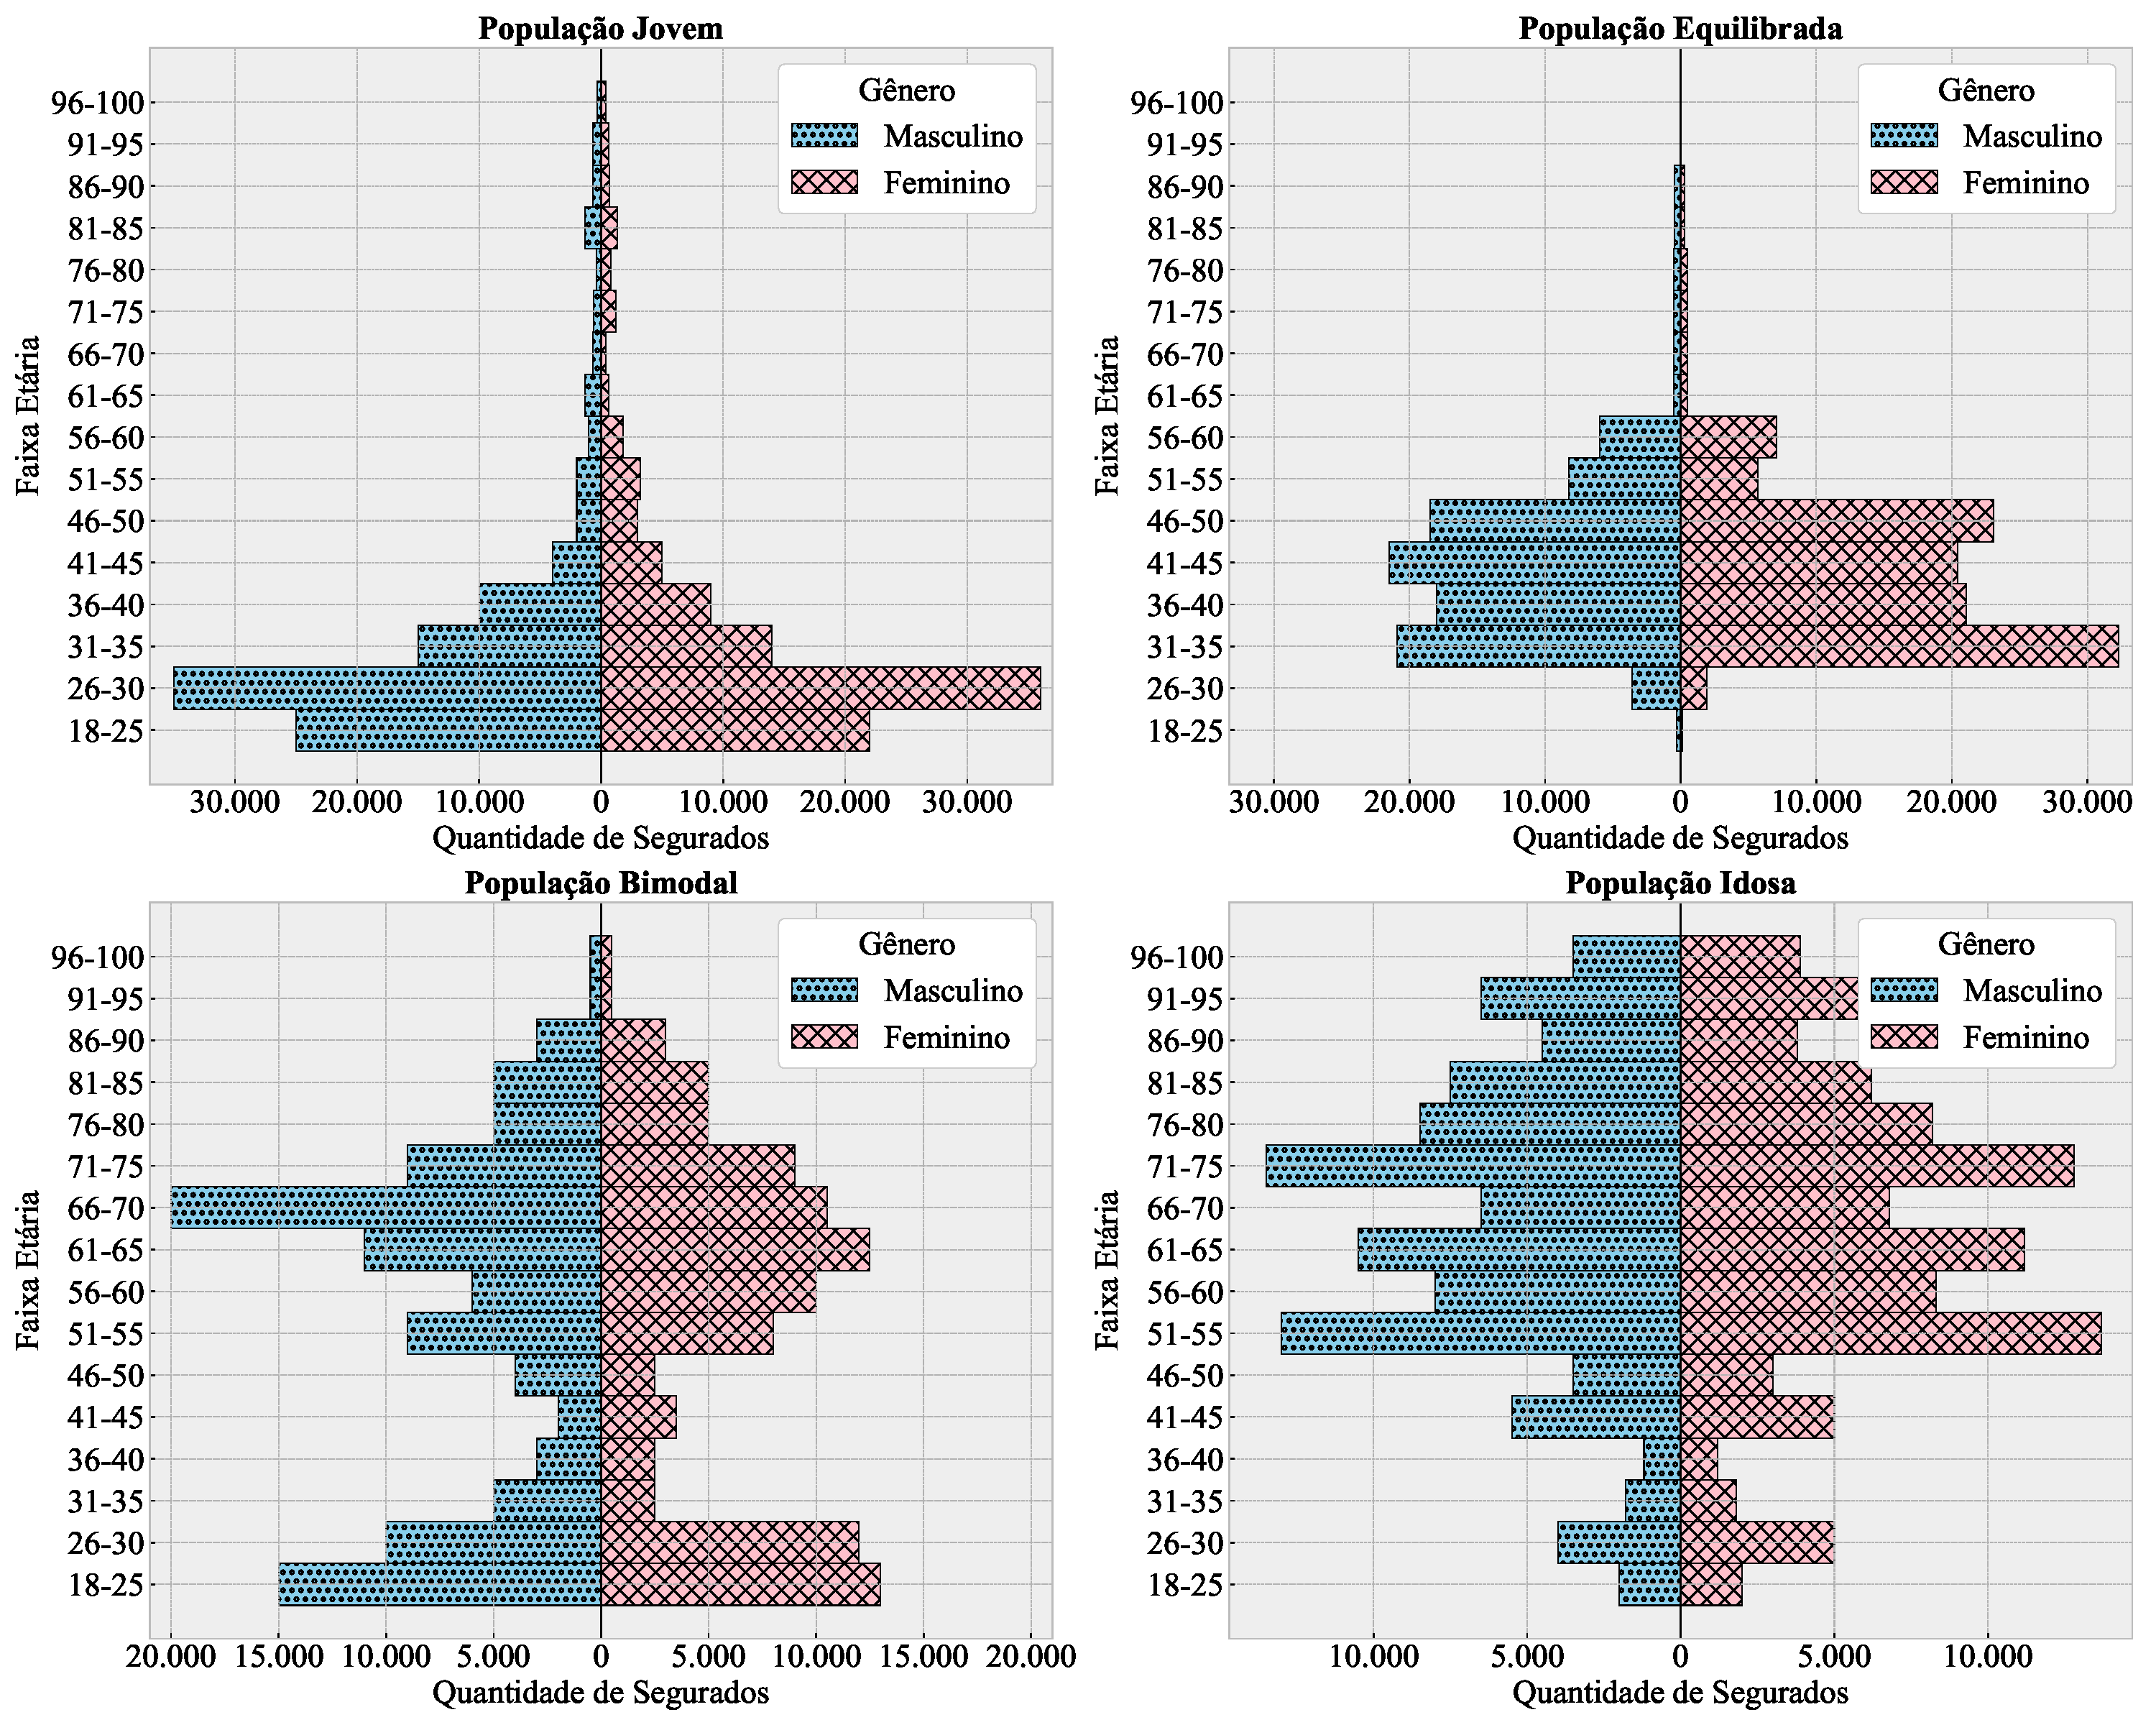
\includegraphics[width=0.97\textwidth]{piramides_etarias.pdf}
    \fonte{Elaboração própria (2026).}
    \label{fig:piramides}
\end{figure}

O perfil jovem simulado é evidênciado com a pirâmide etária superior esquerda contida na Figura \ref{fig:piramides}. A maior concentração de segurados encontra-se nas faixas de 18 a 30 anos, que representam aproximadamente $60\%$ da população masculina e $58\%$ da feminina. A massa equilibrada, representada pela pirâmide superior direito na Figura \ref{fig:piramides} possui uma distribuição mais homogênea, com concentrações relevantes nas faixas centrais (entre 31 e 50 anos). Para as mulheres, observa-se um pico significativo na faixa de 31-35 anos ($32,3\%$), enquanto os homens apresentam uma distribuição mais plana entre os 31 e 50 anos.

O perfil idoso mostrada na pirâmide inferior direita da Figura \ref{fig:piramides} representa um regime com ausência prolongada de novos concursos, esta massa concentra a maioria de seus segurados acima dos 51 anos. Notavelmente, as faixas de 71-75 anos e de 91-95 anos apresentam pesos significativos. A massa bimodal, evidenciada pela pirâmide inferior esquerda da Figura \ref{fig:piramides}, representa o cenário de um RPPS que passou por um longo período de interrupção de contratações, seguido por um certame recente de grande porte.

A Tabela \ref{tab:estatisticas_descritivas} apresenta as principais estatísticas  descritivas das quatro massas seguradas simuladas. O indicador de maturidade da  massa, definido como a razão entre o número de segurados em fase contributiva  (homens com idade inferior a 65 anos e mulheres com idade inferior a 62 anos) e  o número de segurados em fase de percepção de benefícios, sintetiza o grau de  equilíbrio demográfico de cada base.

\vspace{0.25cm}
\begin{table}[htbp]
    \centering
    \caption{Estatísticas Descritivas das Massas Seguradas Simuladas}
    \renewcommand{\arraystretch}{1.2}
    \begin{tabular}{lrrrr}
    \toprule
    \multicolumn{1}{c}{\textbf{Estatística}} & \multicolumn{1}{c}{\textbf{Jovem}} & \multicolumn{1}{c}{\textbf{Equilibrada}} & \multicolumn{1}{c}{\textbf{Bimodal}} & \multicolumn{1}{c}{\textbf{Idosa}} \\
    \midrule
    Idade Média              & 33,57  & 42,54  & 54,15  & 65,13  \\
    Idade Mediana            & 29,00  & 42,00  & 59,00  & 65,00  \\
    Idade Mínima             & 19,00  & 19,00  & 19,00  & 19,00  \\
    1º Quartil               & 26,00  & 35,00  & 32,00  & 53,00  \\
    2º Quartil               & 29,00  & 42,00  & 59,00  & 65,00  \\
    3º Quartil               & 36,00  & 48,00  & 70,00  & 78,00  \\
    Idade Máxima             & 100,00 & 100,00 & 100,00 & 100,00 \\
    Maturidade da Massa      & 17,44  & 41,18  &  1,35  &  0,81  \\
    \bottomrule
    \end{tabular}
    \label{tab:estatisticas_descritivas}
    \vspace{0.25cm}
    \fonte{Elaboração própria (2026).}
\end{table}

A base jovem, com idade média de $33{,}57$ anos e mediana de $29{,}00$ anos, apresenta a maior assimetria positiva entre as duas medidas de tendência central, indicando que uma parcela de segurados em idades mais avançadas eleva a média acima da concentração efetiva da distribuição. O 1º e o 3º quartis, de $26$ e $36$ anos respectivamente, confirmam a forte concentração nas faixas etárias mais jovens. O indicador de maturidade de $17{,}44$ revela que, para cada segurado em fase de benefício, existem aproximadamente $17$ segurados em fase contributiva, configurando um cenário de expressiva folga financeira e baixa pressão imediata sobre o passivo.

A base equilibrada, ainda que apresente uma razão de maturidade superior ($41{,}18$), registra idade média de $42{,}54$ anos e a maior simetria entre média e mediana ($42{,}54$ e $42{,}00$, respectivamente), com amplitude interquartílica de $13$ anos (entre $35$ e $48$ anos). A elevada maturidade decorre da concentração etária nas faixas centrais, que ainda se situam predominantemente abaixo dos limiares de aposentadoria, resultando em reduzida massa de beneficiários em termos absolutos.

A base bimodal apresenta as características mais distintas do conjunto. A amplitude interquartílica de $38$ anos --- do 1º quartil de $32$ anos ao 3º quartil de $70$ anos --- é a maior entre as quatro massas e reflete a estrutura com dois grupos populacionais bem definidos, um grupo de segurados jovens recentemente ingressos e um grupo idoso em iminente ou já concedida aposentadoria. A diferença entre mediana ($59{,}00$) e média ($54{,}15$) indica que o grupo jovem, embora numericamente relevante, não é suficiente para deslocar a mediana para abaixo dos $50$ anos. O indicador de maturidade de $1{,}35$ sinaliza que a base já se encontra próxima ao equilíbrio entre ativos e inativos, com ligeira predominância contributiva.

Por fim, a base idosa apresenta a maior idade média ($65{,}13$ anos) e a maior coincidência entre média e mediana, indicando uma distribuição etária praticamente simétrica em torno de uma faixa de alta senioridade. Com 1º quartil de $53$ anos e 3º quartil de $78$ anos, a massa apresenta baixíssima presença de segurados jovens. O indicador de maturidade de $0{,}81$ é o único inferior à unidade, confirmando que a base idosa é a única em que os beneficiários já superam numericamente os contribuintes, caracterizando o cenário de maior pressão sobre o passivo atuarial e de maior sensibilidade às premissas de mortalidade nas idades avançadas.

\section{\textbf{Provisões matemáticas e inconsistências}}

Esta seção apresenta os resultados das provisões matemáticas calculadas de acordo com as premissas contidas no Quadro \ref{qua:hipoteses_atuariais}. Para cada base de dados simulada, foram calculadas as PM segundo os métodos de custeio INE, CUP e PNI, confrontando-se cada tábua comparativa com a tábua de referência. Uma tábua é classificada como inconsistente quando apresenta expectativa de vida na idade média superior à da tábua de referência e, concomitantemente, produz uma PM inferior à gerada pela tábua de referência.

% --------------------- Base Jovem --------------------------------------
As Tabelas \ref{tab:jovem-ine}, \ref{tab:jovem-CUP} e \ref{tab:jovem-pni} apresentam, respectivamente, os resultados para a base jovem nos métodos INE, CUP e PNI. Em todos os casos, a primeira linha de cada gênero corresponde à tábua de referência (IBGE 2024 Extrapolada), cujo valor de PM serve de parâmetro para identificar as inconsistências. As demais tábuas contidas nessas tabelas registraram uma PM inferior àquela gerada pela tábua de referência. Além disso, são apresentadas as respectivas expectativas de vida na idade média associadas a cada tábua.
\vspace{0.25cm}
\begin{table}[htbp]
    \centering
    \caption{Provisões Matemáticas - Base Jovem - Método INE}
    \begin{threeparttable}
    \renewcommand{\arraystretch}{1.0}
    \begin{tabular}{llrr}
    \toprule
    \multicolumn{1}{c}{\textbf{Gênero}} & \multicolumn{1}{c}{\textbf{Tábua}} & \multicolumn{1}{c}{\textbf{PM}} & \multicolumn{1}{c}{\textbf{$e_{33}$}} \\ \midrule
    \multirow{11}{*}{Masculino} & IBGE 2024 Extrapolada Masculina & 45.598.237,44	& 43,55 \\
                                & IBGE 2019 Extrapolada Ambos Agravada em 19\% & 45.534.229,61 & 43,60 \\
                                & AT-2000 Masculina Agravada em 33\% & 44.909.930,94 & 44,14 \\
                                & AT-55 & 43.848.527,38 & 43,60 \\
                                & AT-55 Suavizada em 5\% & 44.906.722,62 & 44,15 \\
                                & AT-83 Basic Masculina & 44.396.709,59 & 44,13 \\
                                & AT-83 Basic Masculina Suavizada em 2,5\% & 44.896.625,32 & 44,39 \\
                                & BR-EMSmt-v.2021 Masculina Agravada em 24\% & 44.994.744,87 & 44,05 \\
                                & GKM-95 & 43.927.302,57 & 43,59 \\
                                & Prudential-50 Suavizada em 16\% & 45.585.859,77 & 44,26 \\ 
                                & M-95 H Suavizada em 6\% & 44.714.222,92 & 43,95 \\ \hline
    \multirow{4}{*}{Feminino} & IBGE 2024 Extrapolada Feminina & 66.937.295,03	 & 48,70 \\
                                & BR-EMSmt-v.2021 Feminina Agravada em 21,5\% & 66.839.871,57 & 48,84 \\
                                & GAM-71 Feminina & 66.551.189,09 & 48,87 \\
                                & Petros Suavizada em 13\% & 66.228.077,79 & 48,71 \\ \bottomrule
    \end{tabular}
    \begin{tablenotes}[flushleft]
        \small
        \item Fonte: Elaboração própria (2026).
    \end{tablenotes}
    \end{threeparttable}
    \label{tab:jovem-ine}
\end{table}
\vspace{0.5cm}
\begin{table}[htbp]
    \centering
    \caption{Provisões Matemáticas - Base Jovem - Método CUP}
    \begin{threeparttable}
    \renewcommand{\arraystretch}{1.0}
    \begin{tabular}{llrr}
    \toprule
    \multicolumn{1}{c}{\textbf{Gênero}} & \multicolumn{1}{c}{\textbf{Tábua}} & \multicolumn{1}{c}{\textbf{PM}} & \multicolumn{1}{c}{\textbf{$e_{33}$}} \\ \midrule
    \multirow{9}{*}{Masculino} & IBGE 2024 Extrapolada Masculina & 33.299.758,59	& 43,55 \\
                    & AT-2000 Masculina Agravada em 33\% & 32.678.511,80 & 44,14 \\
                    & AT-55 & 32.048.662,32	& 43,60 \\
                    & AT-55 Suavizada 5\% & 32.825.920,09 & 44,15 \\
                    & AT-83 Basic Masculina & 32.327.043,98 & 44,13 \\
                    & AT-83 Basic Masculina Suavizada 2,5\% & 32.694.946,44 & 44,39 \\
                    & BR-EMSmt-v.2021 Masculina Agravada em 24\% & 32.776.498,80 & 44,05 \\
                    & GKM-95 & 32.032.418,81 & 43,59 \\
                    & M-95 H Suavizada 6\% & 32.536.096,19 & 43,95 \\ \hline
    \multirow{4}{*}{Feminino} & IBGE 2024 Extrapolada Feminina & 49.671.069,71 & 48,70 \\
                                & BR-EMSmt-v.2021 Feminina Agravada em 21,5\% & 49.654.760,02 & 48,84 \\
                                & GAM-71 Feminina & 49.246.868,07 & 48,87 \\ 
                        & Petros Suavizada 13\% & 49.121.704,09 & 48,71 \\ \bottomrule
    \end{tabular}
    \begin{tablenotes}[flushleft]
        \small
        \item Fonte: Elaboração própria (2026).
    \end{tablenotes}
    \end{threeparttable}
    \label{tab:jovem-CUP}
\end{table}

\begin{table}[htbp]
    \centering
    \caption{Provisões Matemáticas - Base Jovem - Método PNI}
    \begin{threeparttable}
    \renewcommand{\arraystretch}{1.0}
    \begin{tabular}{llrr}
    \toprule
    \multicolumn{1}{c}{\textbf{Gênero}} & \multicolumn{1}{c}{\textbf{Tábua}} & \multicolumn{1}{c}{\textbf{PM}} & \multicolumn{1}{c}{\textbf{$e_{33}$}} \\ \midrule
    \multirow{13}{*}{Masculino}
    & IBGE 2024 Extrapolada Masculina                  & 30.208.928,00 & 43,55 \\
    & IBGE 2019 Extrapolada Ambos Agravada em 19\%      & 29.866.462,94 & 43,60 \\
    & IBGE 2019 Extrapolada Ambos Agravada em 18,3\%    & 29.976.475,14 & 43,70 \\
    & AT-2000 Masculina Agravada em 33\%               & 28.611.697,60 & 44,14 \\
    & AT-55                               & 27.915.473,47 & 43,60 \\
    & AT-55 Suavizada em 5\%                     & 28.575.622,26 & 44,15 \\
    & AT-83 Basic Masculina                       & 27.976.902,86 & 44,13 \\
    & AT-83 Basic Masculina Suavizada em 2,5\%           & 28.290.738,39 & 44,39 \\
    & BR-EMSmt-v.2021 Masculina Agravada em 24\%        & 28.974.636,30 & 44,05 \\
    & GKM-95                              & 28.451.524,37 & 43,59 \\
    & Prudential-50 Suavizada em 16\%            & 29.189.236,82 & 44,26 \\
    & TR 2025                             & 29.985.619,04 & 43,84 \\
    & M-95 H Suavizada em 6\%                    & 28.925.074,93 & 43,95 \\ \hline
    \multirow{5}{*}{Feminino}
    & IBGE 2024 Extrapolada Feminina                  & 40.739.430,62 & 48,70 \\
    & BR-EMSmt-v.2021 Feminina Agravada em 21,5\%     & 40.676.942,28 & 48,84 \\
    & GAM-71 Feminina                            & 39.948.430,84 & 48,87 \\
    & GAM-71 Feminina Suavizada em 5\%                   & 40.556.722,03 & 49,36 \\
    & Petros Suavizada em 13\%               & 39.854.702,97 & 48,71 \\ \bottomrule
    \end{tabular}
    \begin{tablenotes}[flushleft]
        \small
        \item Fonte: Elaboração própria (2026).
    \end{tablenotes}
    \end{threeparttable}
    \label{tab:jovem-pni}
\end{table}
\FloatBarrier
A base jovem é a mais suscetível à ocorrência de inconsistências dentre as quatro bases analisadas. Nos métodos INE e CUP, verificam-se 10 e 8 tábuas inconsistentes para o sexo masculino, respectivamente, e 3 tábuas para o sexo feminino em ambos os métodos. Os métodos INE e CUP compartilham as mesmas tábuas inconsistentes para o sexo feminino, diferindo apenas na composição masculina e, naturalmente, nos valores absolutos das provisões.

A análise dos valores absolutos revela que os desvios em relação à tábua de referência podem apresentar níveis mais elevados no gênero masculino. No método INE, a tábua AT-55 masculina produz uma PM de R\$43.848.527,38, o que representa uma redução de aproximadamente 3,8\% em relação à referência. A tábua GKM-95 apresenta uma magnitude similar, enquanto as tábuas AT-83 Basic masculina e AT-2000 masculina agravada em 33\% ficam cerca de 2,6\% abaixo da referência. Para o sexo feminino, as reduções são relativamente menores em termos percentuais, com a tábua Petros suavizada 13\% registrando um desvio de aproximadamente 1,1\% abaixo da referência e a GAM-71 feminina em torno de 0,6\%.

O método PNI apresentou o maior número de tábuas que registram inconsistências, dentre os três métodos de custeio. Sendo 12 tábuas para o sexo masculino e 4 para o feminino, totalizando 16 ocorrências. Além de incorporar todas as tábuas já inconsistentes no INE e no CUP, acrescenta as tábuas IBGE 2019 Extrapalotada ambos agravada em 18,3\%, TR 2025 no gênero masculino e a tábua GAM-71 Feminina suavizada em 5\% no gênero feminino. Nos casos masculinos adicionais, os desvios em relação à referência do PNI variam entre 0,8\% e 7,6\%. Essa maior propensão do PNI às inconsistências pode estar relacionada ao papel da premissa de crescimento salarial no cálculo do VACF, que eleva o custo normal futuro sem contrapartida proporcional no VABF.

% -------------------- Base Equilibrada ---------------------------------
A Tabela \ref{tab:equilibrada-ine} apresenta os resultados para a base equilibrada utilizando o método INE, e a Tabela \ref{tab:equilibrada-CUP} os resultados pelo método CUP, ambas seguindo a mesma estrutura das tabelas referentes à base jovem, segmentadas por sexo e por tábua de mortalidade. A Tabela \ref{tab:equilibrada-pni} consolida os resultados do método PNI para a mesma base.
\vspace{0.25cm}
\begin{table}[htbp]
    \centering
    \caption{Provisões Matemáticas - Base Equilibrada - Método INE}
    \begin{threeparttable}
    \renewcommand{\arraystretch}{1.0}
    \begin{tabular}{llrr}
    \toprule
    \multicolumn{1}{c}{\textbf{Gênero}} & \multicolumn{1}{c}{\textbf{Tábua}} & \multicolumn{1}{c}{\textbf{PM}} & \multicolumn{1}{c}{\textbf{$e_{42}$}} \\ \midrule
    \multirow{8}{*}{Masculino} & IBGE 2024 Extrapolada Masculina & 86.592.641,91	& 35,57 \\
                                & IBGE 2019 Extrapolada Ambos Agravada em 18,3\% & 86.513.760,50 & 35,60 \\
                                & AT-2000 Masculina Agravada em 33\% & 85.822.340,72 & 35,61 \\
                                & AT-55 Suavizada em 5\% & 85.124.399,51 & 35,67 \\
                                & AT-83 Basic Masculina Suavizada em 2,5\% & 85.663.646,44 & 35,77 \\
                                & BR-EMSmt-v.2021 Masculina Agravada em 24\% & 85.792.211,27 & 35,80 \\
                                & Prudential-50 Suavizada em 16\% & 85.610.897,19 & 35,74 \\
                                & M-95 H Suavizada em 6\% & 85.343.574,38 & 35,63 \\ \hline
    \multirow{5}{*}{Feminino} & IBGE 2024 Extrapolada Feminina& 134.568.492,31 & 40,20 \\
                                & BR-EMSmt-v.2021 Feminina Agravada em 21,5\% & 134.017.399,15 & 40,24 \\
                                & IBGE 2019 Extrapolada Ambos Suavizada em 19\% & 133.729.335,87 & 40,26 \\
                                & IBGE 2019 Extrapolada Feminina & 134.144.047,75 & 40,31 \\
                                & Petros Suavizada em 15\% & 134.172.115,72 & 40,24 \\ \bottomrule
    \end{tabular}
    \begin{tablenotes}[flushleft]
        \small
        \item Fonte: Elaboração própria (2026).
    \end{tablenotes}
    \end{threeparttable}
    \label{tab:equilibrada-ine}
\end{table}
\vspace{0.25cm}
\begin{table}[htbp]
    \centering
    \caption{Provisões Matemáticas - Base Equilibrada - Método CUP}
    \begin{threeparttable}
    \renewcommand{\arraystretch}{1.0}
    \begin{tabular}{llrr}
    \toprule
    \multicolumn{1}{c}{\textbf{Gênero}} & \multicolumn{1}{c}{\textbf{Tábua}} & \multicolumn{1}{c}{\textbf{PM}} & \multicolumn{1}{c}{\textbf{$e_{42}$}} \\ \midrule
    \multirow{7}{*}{Masculino} & IBGE 2024 Extrapolada Masculina & 64.800.294,08 & 35,57 \\
                                & AT-2000 Masculina Agravada em 33\% & 64.329.635,17 & 35,61 \\
                                & AT-55 Suavizada em 5\% & 63.895.755,13 & 35,67 \\
                                & AT-83 Basic Masculina Suavizada em 2,5\% & 64.275.168,12 & 35,77 \\
                                & BR-EMSmt-v.2021 Masculina Agravada em 24\% & 64.298.694,54 & 35,80 \\
                                & Prudential-50 Suavizada em 16\% & 64.334.991,35 & 35,74 \\
                                & M-95 H Suavizada em 6\% & 63.934.265,30 & 35,63 \\ \hline
    \multirow{5}{*}{Feminino} & IBGE 2024 Extrapolada Feminina & 103.405.148,42 & 40,20 \\
                                & BR-EMSmt-v.2021 Feminina Agravada em 21,5\% & 103.050.238,14 & 40,24\\
                                & IBGE 2019 Extrapolada Ambos Suavizada em 19\% & 102.734.846,74 & 40,26 \\
                                & IBGE 2019 Extrapolada Feminina & 103.136.629,05 & 40,31 \\
                                & Petros Suavizada em 15\% & 103.199.979,88 & 40,24 \\ \bottomrule
    \end{tabular}
    \begin{tablenotes}[flushleft]
        \small
        \item Fonte: Elaboração própria (2026).
    \end{tablenotes}
    \end{threeparttable}
    \label{tab:equilibrada-CUP}
\end{table}
\newpage
\begin{table}[htbp]
    \centering
    \caption{Provisões Matemáticas - Base Equilibrada - Método PNI}
    \begin{threeparttable}
    \renewcommand{\arraystretch}{1.0}
    \begin{tabular}{llrr}
    \toprule
    \multicolumn{1}{c}{\textbf{Gênero}} & \multicolumn{1}{c}{\textbf{Tábua}} & \multicolumn{1}{c}{\textbf{PM}} & \multicolumn{1}{c}{\textbf{$e_{42}$}} \\ \midrule
    \multirow{9}{*}{Masculino} & IBGE 2024 Extrapolada Masculina & 56.021.464,81 & 35,57 \\
                                & IBGE 2021 Extrapolada Masculina Suavizada em 1\% & 55.965.974,66 & 35,59 \\
                                & IBGE 2019 Extrapolada Ambos Agravada em 18,3\% & 55.257.406,12 & 35,60 \\
                                & AT-2000 Masculina Agravada em 33\% & 53.406.025,67	 & 35,61 \\
                                & AT-55 Suavizada em 5\% & 52.743.177,24 & 35,67 \\
                                & AT-83 Basic Masculina Suavizada em 2,5\% & 52.696.171,78 & 35,77 \\
                                & BR-EMSmt-v.2021 Masculina Agravada em 24\% & 53.939.039,81 & 35,68 \\
                                & Prudential-50 Suavizada em 16\% & 52.989.127,02 & 35,74 \\
                                & M-95 H Suavizada em 6\% & 53.950.903,39 & 35,63 \\ \hline
    \multirow{6}{*}{Feminino} & IBGE 2024 Extrapolada Feminina & 67.200.062,13 & 40,20 \\
                                & BR-EMSmt-v.2021 Feminina Agravada em 21,5\% & 66.593.617,83 & 40,24 \\
                                & GAM-71 Feminina Suavizada em 5\% & 66.885.152,17 & 40,65 \\
                                & IBGE 2020 Extrapolada Feminina & 67.169.586,38 & 40,48 \\
                                & IBGE 2019 Extrapolada Feminina & 66.911.376,98 & 40,31 \\ 
                                & Petros Suavizada em 15\% & 65.811.523,35 & 40,24 \\ \bottomrule
    \end{tabular}
    \begin{tablenotes}[flushleft]
        \small
        \item Fonte: Elaboração própria (2026).
    \end{tablenotes}
    \end{threeparttable}
    \label{tab:equilibrada-pni}
\end{table}

Ao confrontar os resultados das Tabelas \ref{tab:equilibrada-ine} e \ref{tab:equilibrada-CUP}, observa-se que os métodos INE e CUP voltam a compartilhar as mesmas tábuas inconsistentes para o sexo feminino. Para o sexo masculino, ambos identificam o mesmo conjunto de seis tábuas inconsistentes, com exceção da IBGE 2019 Extrapolada Ambos agravada em 18,3\%, presente apenas no INE. Em termos percentuais, a tábua AT-55 suavizada em 5\% gera o maior desvio, de aproximadamente 1,7\% abaixo da referência no INE e 1,4\% no CUP. 

A tábua M-95 H suavizada em 6\% situa-se em 1,4\% abaixo da referência no INE e 1,3\% no CUP. Para o sexo feminino, os desvios são menores. A IBGE 2019 Extrapolada Ambos suavizada em 19\% fica 0,6\% abaixo da referência no INE e no CUP. É notável que, na base equilibrada, o número total de inconsistências nos métodos INE e CUP, 7 e 6 tábuas masculinas, respectivamente, e 4 femininas em ambos, é inferior ao observado na base jovem, indicando que o envelhecimento gradual da população já reduz a exposição ao risco de subestimação da PM.

Os resultados da Tabela \ref{tab:equilibrada-pni} confirmam a maior suscetibilidade do método PNI, registrando 8 tábuas inconsistentes masculinas e 5 femininas, superando os totais registrados nos métodos INE e CUP. Além de incorporar todas as tábuas identificadas nesses dois métodos, o PNI acrescenta a IBGE 2021 Extrapolada Masculina suavizada em 1\%, para o gênero masculino, e a GAM-71 Feminina suavizada em 5\% e IBGE 2020 Extrapolada Feminina, para o gênero feminino. Os desvios mais acentuados no PNI são os da AT-83 Basic M suavizada em 2,5\% e da AT-55 suavizada em 5\% no sexo masculino, com 5,9\% e 5,8\% abaixo da referência, respectivamente. Para o sexo feminino, o maior desvio abaixo da referência cabe à Petros suavizada 15\% com 2,1\%.

Observe-se ainda que tábuas de origem do IBGE figuram entre as inconsistentes no método PNI, o que indica que o problema não se restringe apenas a tábuas antigas. Essa constatação contrasta com a possível interpretação inicial decorrente da presença recorrente de tábuas antigas, como AT-55 e AT-83, bem como de algumas ocorrências, ainda que menos frequentes, de outras tábuas antigas, como a GKM-95.

% ------------------------ Base Bimoda ----------------------------------
As Tabelas~\ref{tab:bimodal-ine}, \ref{tab:bimodal-CUP} e~\ref{tab:bimodal-pni} apresentam os resultados para a base bimodal nos métodos INE, CUP e PNI, respectivamente. Todas seguem a mesma estrutura de apresentação detalhada nas tabelas da base jovem.
\vspace{0.25cm}
\begin{table}[htbp]
    \centering
    \caption{Provisões Matemáticas - Base Bimodal - Método INE}
    \begin{threeparttable}
    \renewcommand{\arraystretch}{1.0}
    \begin{tabular}{llrr}
    \toprule
    \multicolumn{1}{c}{\textbf{Gênero}} & \multicolumn{1}{c}{\textbf{Tábua}} & \multicolumn{1}{c}{\textbf{PM}} & \multicolumn{1}{c}{\textbf{$e_{54}$}} \\ \midrule
    \multirow{2}{*}{Masculino} & IBGE 2024 Extrapolada Masculina & 188.588.249,67 & 25,44 \\
                                & IBGE 2019 Extrapolada Ambos Agravada em 18,3\% & 188.516.635,07 & 25,45 \\ \hline
    \multirow{2}{*}{Feminino} & IBGE 2024 Extrapolada Feminina & 203.454.768,85 & 29,31 \\
                                & GAM-71 Feminina Suavizada em 5\% & 201.542.054,08 & 29.35 \\ \bottomrule
    \end{tabular}
    \begin{tablenotes}[flushleft]
        \small
        \item Fonte: Elaboração própria (2026).
    \end{tablenotes}
    \end{threeparttable}
    \label{tab:bimodal-ine}
\end{table}
\vspace{0.5cm}
\begin{table}[htbp]
    \centering
    \caption{Provisões Matemáticas - Base Bimodal - Método CUP}
    \begin{threeparttable}
    \renewcommand{\arraystretch}{1.0}
    \begin{tabular}{llrr}
    \toprule
    \multicolumn{1}{c}{\textbf{Gênero}} & \multicolumn{1}{c}{\textbf{Tábua}} & \multicolumn{1}{c}{\textbf{PM}} & \multicolumn{1}{c}{\textbf{$e_{54}$}} \\ \midrule
    \multirow{2}{*}{Masculino} & IBGE 2024 Extrapolada Masculina & 178.462.070,71 & 25,44 \\
                                & IBGE 2019 Extrapolada Ambos Agravada em 18,3\% & 178.429.558,25 & 25,45 \\ \hline
    \multirow{2}{*}{Feminino} & IBGE 2024 Extrapolada Feminina & 192.985.155,19 & 30,19 \\
                                & GAM-71 Feminina Suavizada em 5\% & 191.079.527,54 & 30,28 \\ \bottomrule
    \end{tabular}
    \begin{tablenotes}[flushleft]
        \small
        \item Fonte: Elaboração própria (2026).
    \end{tablenotes}
    \end{threeparttable}
    \label{tab:bimodal-CUP}
\end{table}
\vspace{0.5cm}
\begin{table}[htbp]
    \centering
    \caption{Provisões Matemáticas - Base Bimodal - Método PNI}
    \begin{threeparttable}
    \renewcommand{\arraystretch}{1.0}
    \begin{tabular}{llrr}
    \toprule
    \multicolumn{1}{c}{\textbf{Gênero}} & \multicolumn{1}{c}{\textbf{Tábua}} & \multicolumn{1}{c}{\textbf{PM}} & \multicolumn{1}{c}{\textbf{$e_{54}$}} \\ \midrule
    \multirow{7}{*}{Masculino} & IBGE 2024 Extrapolada Masculina & 139.594.842,64 & 25,44 \\
                                & IBGE 2019 Extrapolada Ambos Agravada em 18,3\% & 138.626.920,52 & 25.45 \\
                                & Prudential-50 Suavizada em 18\% & 136.033.436,19 & 25,44 \\
                                & RP-2000 Masculina & 133.445.341,21 & 27.09 \\
                                & UP - 94 Masculina & 133.503.335,30 & 26.38 \\
                                & Petros & 139.005.142,96 & 27,58 \\ \hline
    \multirow{4}{*}{Feminino} & IBGE 2024 Extrapolada Feminina & 136.870.094,98 & 29,31	\\
                                & AT-83 Basic Feminina & 136.147.741,41 & 30,25\\
                                & GAM-71 Feminina Suavizada em 5\% & 132.629.305,17 & 29,35 \\
                                & RP-2000 F & 135.003.551,03 & 29,84 \\ \bottomrule
    \end{tabular}
    \begin{tablenotes}[flushleft]
        \small
        \item Fonte: Elaboração própria (2026).
    \end{tablenotes}
    \end{threeparttable}
    \label{tab:bimodal-pni}
\end{table}

A base bimodal apresenta comportamento mais retraído em relação ao número de tábuas inconsistentes, nos métodos INE e CUP, com apenas uma tábua inconsistente por gênero em cada método. Nos métodos INE e CUP, os desvios em relação à referência são muito reduzidos em comparação com os devios anteriores. A tábua IBGE 2019 Extrapolda Ambos agravada em 18,3\%, para o sexo masculino, fica apenas 0,04\% abaixo da referência no INE e 0,02\% no CUP. Para o sexo feminino, a GAM-71 Feminina suavizada em 5\% registra um desvio abaixo da referência de 0,94\% no INE e 0,99\% no CUP. A pequena magnitude dos desvios nos métodos INE e CUP sugere que, embora a inconsistência exista e seja formalmente detectável, seu impacto financeiro seria mais limitado nesse perfil etário do que nas bases jovem e equilibrada.

O método PNI, contudo, volta a ampliar significativamente o número de inconsistências, registrando 5 tábuas masculinas e 3 femininas inconsistentes. As tábuas RP-2000 M, UP-94 M e Petros aparecem para o gênero masculino, bem como AT-83 Basic Feminina e RP-2000 Feminina aparecem no gênero feminino. Tais tábuas surgem nesse contexto com desvios mais expressivos. A tábua RP-2000 M fica 4,4\% abaixo da referência no PNI, e AT-83 Basic Feminina registra 0,5\%. Nota-se também que, na base bimodal, o PNI é o método que concentra maior número de inconsistências em tábuas sem qualquer suavização ou agravamento, a exemplo das tábuas RP-2000 M, UP-94 M, Petros e RP-2000 F, indicando que o efeito da premissa de crescimento salarial desse método pode ser suficiente para induzir inconsistências mesmo sem modificações nas tábuas.

% ------------------------ Base Idosa ----------------------------------
As Tabelas~\ref{tab:idosa-ine}, \ref{tab:idosa-CUP} e~\ref{tab:idosa-pni} apresentam, respectivamente, os resultados para a base idosa nos métodos INE, CUP e PNI. Tais tabelas seguem a mesma sistemática de apresentação da base jovem.
\vspace{0.25cm}
\begin{table}[htbp]
    \centering
    \caption{Provisões Matemáticas - Base Idosa - Método INE}
    \begin{threeparttable}
    \renewcommand{\arraystretch}{1.0}
    \begin{tabular}{llrr}
    \toprule
    \multicolumn{1}{c}{\textbf{Gênero}} & \multicolumn{1}{c}{\textbf{Tábua}} & \multicolumn{1}{c}{\textbf{PM}} & \multicolumn{1}{c}{\textbf{$e_{65}$}} \\ \midrule
    \multirow{2}{*}{Masculino} & IBGE 2024 Extrapolada Masculina & 191.461.839,97 & 17,21 \\
                                & TR 2025 & 191.229.462,89 & 17.48 \\ \hline
    \multirow{2}{*}{Feminino} & IBGE 2024 Extrapolada Feminina & 238.707.049,45 & 20,07 \\
                                & M-95 M Suavizada em 7\% & 238.267.438,63 & 20,08 \\ \bottomrule
    \end{tabular}
    \begin{tablenotes}[flushleft]
        \small
        \item Fonte: Elaboração própria (2026).
    \end{tablenotes}
    \end{threeparttable}
    \label{tab:idosa-ine}
\end{table}
\vspace{0.25cm}
\begin{table}[htbp]
    \centering
    \caption{Provisões Matemáticas - Base Idosa - Método CUP}
    \begin{threeparttable}
    \renewcommand{\arraystretch}{1.0}
    \begin{tabular}{llrr}
    \toprule
    \multicolumn{1}{c}{\textbf{Gênero}} & \multicolumn{1}{c}{\textbf{Tábua}} & \multicolumn{1}{c}{\textbf{PM}} & \multicolumn{1}{c}{\textbf{$e_{65}$}} \\ \midrule
    \multirow{2}{*}{Masculino} & IBGE 2024 Extrapolada Masculina & 181.074.602,87 & 17,21 \\
                                & TR 2025 & 180.667.661,13 & 17,48 \\ \hline
    \multirow{2}{*}{Feminino} & IBGE 2024 Extrapolada Feminina & 227.062.922,78 & 20,07 \\
                                & M-95 M Suavizada em 7\% & 226.560.063,34 & 20,08 \\ \bottomrule
    \end{tabular}
    \begin{tablenotes}[flushleft]
        \small
        \item Fonte: Elaboração própria (2026).
    \end{tablenotes}
    \end{threeparttable}
    \label{tab:idosa-CUP}
\end{table}

\vspace{0.5cm}
As Tabelas \ref{tab:idosa-ine} e \ref{tab:idosa-CUP} mostram que a base idosa, nos métodos INE e CUP, apresenta apenas uma tábua inconsistente por gênero em cada método, seguindo o comportamento da base bimodal. Os desvios em relação à referência também são menores. A tábua TR 2025 masculina fica apenas 0,12\% abaixo da referência no INE e 0,22\% no CUP. Analogamente, a M-95 M suavizada em 7\% feminina registra desvio de 0,18\% abaixo da referência no INE e 0,22\% no CUP. Esta pequena magnitude reflete o perfil predominantemente aposentado da base idosa. Como os benefícios já estão em sua maioria concedidos (o VABF responde de forma dominante ao valor total da PM), a variação da sobrevivência nas idades contributivas, que afeta o VACF, perde um pouco de relevância. Tal características desse perfil etário pode atuar como um filtro natural, reduzindo drasticamente a janela para a ocorrência de inconsistências.
\vspace{0.25cm}
\begin{table}[htbp]
    \centering
    \caption{Provisões Matemáticas - Base Idosa - Método PNI}
    \begin{threeparttable}
    \renewcommand{\arraystretch}{1.2}
    \begin{tabular}{llrr}
    \toprule
    \multicolumn{1}{c}{\textbf{Gênero}} & \multicolumn{1}{c}{\textbf{Tábua}} & \multicolumn{1}{c}{\textbf{PM}} & \multicolumn{1}{c}{\textbf{$e_{65}$}} \\ \midrule
    \multirow{6}{*}{Masculino} & IBGE 2024 Extrapolada Masculina & 142.045.316,64 & 17,21 \\
                                & Prudential-50 Suavizada em 19\% & 141.688.127,14 & 17,24 \\
                                & RP-2000 M & 133.815.045,87 & 17,61 \\
                                & UP - 94 M & 135.036.953,10 & 17,26 \\
                                & TR 2025 & 140.142.700,27 & 17,48 \\
                                & Petros & 140.335.549,98 & 18,37 \\ \hline
    \multirow{5}{*}{Feminino} & IBGE 2024 Extrapolada Feminina & 164.441.923,44 & 20,07 \\
                                & AT-83 Basic Feminina & 162.489.690,38 & 20,45 \\
                                & RP-2000 Feminina & 162.749.334,10 & 20,12 \\
                                & CL5 & 164.176.613,09 & 20,98 \\
                                & M-95 M Suavizada em 7\% & 163.617.467,92 & 20,08 \\ \bottomrule
    \end{tabular}
    \begin{tablenotes}[flushleft]
        \small
        \item Fonte: Elaboração própria (2026).
    \end{tablenotes}
    \end{threeparttable}
    \label{tab:idosa-pni}
\end{table}

No método PNI, a base idosa volta a revelar a maior propensão desse método a inconsistências. São 5 tábuas masculinas e 4 femininas, totalizando 9 ocorrências. Os desvios tornam-se expressivos, com a tábua RP-2000 M com 5,8\% abaixo da referência e a UP-94 M com 5,1\% abaixo da referência. Para o sexo feminino, o maior desvio de 1,2\% abaixo da referência é registrado pela AT-83 Basic F, seguida da RP-2000 F com 1,0\%. Chama atenção que a TR 2025 masculina, inconsistente também nos métodos INE e CUP, mantém sua condição no PNI com desvio de 1,3\% abaixo da referência, indicando que essa tábua exibe um diferencial de sobrevivência nas idades de benefício que, combinado com o efeito da premissa de crescimento salarial, é suficiente para reduzir a PM independentemente do método de custeio empregado.

% ---------------------------- Geral ------------------------------------
Por fim, A Tabela \ref{tab:sintese_inconsistencias} consolida o número total de tábuas inconsistentes por base, método e gênero, permitindo uma visão panorâmica dos resultados. Os resultados consolidados na Tabela \ref{tab:sintese_inconsistencias} indicam três padrões de comportamento.
\newpage 

\begin{table}[htbp]
    \centering
    \caption{Número de Tábuas Inconsistentes por Base, Método e Gênero}
    \begin{threeparttable}
    \renewcommand{\arraystretch}{1.1}
    \begin{tabular}{lcccccc}
    \toprule
    & \multicolumn{2}{c}{\textbf{INE}} & \multicolumn{2}{c}{\textbf{CUP}} & \multicolumn{2}{c}{\textbf{PNI}} \\
    \cmidrule(lr){2-3}\cmidrule(lr){4-5}\cmidrule(lr){6-7}
    \textbf{Base} & \textbf{Masc.} & \textbf{Fem.} & \textbf{Masc.} & \textbf{Fem.} & \textbf{Masc.} & \textbf{Fem.} \\
    \midrule
    Jovem       & 10 & 3 & 8 & 3 & 12 & 4 \\
    Equilibrada &  7 & 4 & 6 & 4 &  8 & 5 \\
    Bimodal     &  1 & 1 & 1 & 1 &  5 & 3 \\
    Idosa       &  1 & 1 & 1 & 1 &  5 & 4 \\
    \midrule
    \textbf{Total} & \textbf{19} & \textbf{9} & \textbf{16} & \textbf{9} & \textbf{30} & \textbf{16} \\
    \bottomrule
    \end{tabular}
    \begin{tablenotes}[flushleft]
        \small
        \item Fonte: Elaboração própria (2026).
    \end{tablenotes}
    \end{threeparttable}
    \label{tab:sintese_inconsistencias}
\end{table}

Primeiro, há uma relação inversa entre a idade média da base e o número de inconsistências. A base jovem com uma idade média de 33,57 anos concentra a maior parte das ocorrências, enquanto as bases bimodal e idosa, com idades médias de 54,16 e 65,13 anos respectivamente, registram apenas uma inconsistência por gênero em cada um desses métodos. 

Este resultado indica que estruturas etárias mais jovens podem estar mais suscetíveis a tábuas de mortalidade que apresentem expectativa de vida na idade média superior à da tábua de referência, porém resultando em uma PM inferior àquela gerada pela tábua de referência. Essa divergência corrobora que indicadores isolados de longevidade podem distorcer a mensuração do passivo atuarial \cite{BERGERON2019,fong2015}.

O Segundo comportamento se refere aos métodos de custeio. O método INE e o método CUP compartilham, em todas as bases, o mesmo conjunto de tábuas inconsistentes, com pequenas variações pontuais para o sexo masculino. Já o método PNI demonstra maior propensão a inconsistências em todas as bases. Esse método registra entre 2 e 5 ocorrências masculinas adicionais e entre 0 e 2 femininas adicionais em relação ao INE e CUP.

No total acumulado, o PNI apresenta 30 inconsistências masculinas e 16 femininas, contra 19 e 9 do INE e 15 e 9 no CUP. Essa diferença pode estar ligada à premissa de crescimento salarial embutida no cálculo do VACF nesse método, que eleva o custo normal futuro sem que haja um aumento proporcional no VABF. Esse comportamento sugere que as inconsistências resultam de uma propriedade da combinação tábua–base demográfica, e não uma característica específica de um método, mesmo que o método PNI tenha acentuado o número de inconsistências.

O terceiro comportamento observado está relacionado aos sexos. O sexo masculino apresentou um número maior de tábuas inconsistentes, com exceção das bases bimodal e idosa nos métodos INE e CUP. Esse resultado sugere que, para o sexo masculino, há maior ocorrência de tábuas cuja PM é inferior aquela gerada pela tábua de referência, mesmo quando a expectativa de vida na idade média supera a da tábua de referência. Uma possível explicação para esse resultado está no histórico de variação da mortalidade masculina, que tende a apresentar maior variabilidade ao longo do tempo quando comparada à mortalidade feminina, geralmente considerada mais estável \cite{dif_genero2020}.

Outro ponto a ser observado é o mecanismo de suavização/agravamento de tábuas de mortalidade, no qual algumas tábuas apresentaram PM inferiores àquela gerada pela tábua de referência em suas versões suavizadas ou agravadas. O fato de tábuas como BR-EMSmt-v.2021 M Agravada 24\% e Prudential-50 Suavizada aparecerem repetidamente em diversos métodos, enquanto suas versões originais não aparecem, reforça esse ponto. Na literatura atuarial, sabe-se que as escolhas metodológicas podem alterar substancialmente o capital requerido \cite{palman2017}. No contexto brasileiro, isso sinaliza um risco de “arbitragem atuarial”, onde o RPPS utiliza ajustes técnicos para reduzir o custo imediato sem ferir a literalidade da Portaria.

A análise das simulações, quando confrontada com dados fornecidos pela Secretaria de Previdência Social para o exercício de 2025, mostra uma conexão entre os cenários simulados e o panorama nacional dos RPPS. Observa-se que aproximadamente 1.310 massas seguradas apresentam uma idade média de 33 anos ou 42 anos. Esses perfis etários podem guardar semelhanças com as estruturas da base jovem simulada e da base equilibrada, onde a faixa de 18 a 30 anos concentrava cerca de 60\% dos segurados na base jovem e a faixa 18-35 concentre aproximadamente 57\% dos segurados na base equilibrada. 

Considerando que a idade média informada é próxima à faixa predominante da simulação, é razoável inferir que tais massas reais possuem uma distribuição etária com concentração nas idades iniciais, ainda que com alguma dispersão para faixas posteriores. Ainda que o impacto seja inferior ao observado na base jovem e equilibrada, convém notar que se verifica, a partir da mesma fonte de dados, a existência de cerca de 2.453 massas seguradas com idade média aproximada de 65 anos ou 54 anos, alinhando ao perfil delineado para a base idosa ou para a base bimodal. Diante da similaridade etária entre as massas reais e as bases simuladas, é possível que a adoção de distintas tábuas de mortalidade nessas massas seguradas gere inconsistências semelhantes aquelas observadas nas simulações \cite{brasil_draa_2026}.

\section{\textbf{Fatores explicativos}}

Esta seção se dedica a investigar as inconsistências observadas nos resultados anteriores, primeiramente por meio da análise da curva de $l_x$ para as tábuas comparativas inconsistentes, seguido do cálculo do índice proposto na equação \ref{eq:indice} e sua interpretação.

Na Figura \ref{fig:curva_lx_jovem_masc}, observa-se a curva de $l_x$ para a tábua de referência masculina, bem como para a tábua comparativa inconsistente AT-55 e para a tábua BR-EMSmt 2015 Masculina Agravada em 25\%, que não apresenta inconsistência, uma vez que resultou em valores superiores tanto para $e_{\overline{X}}$ quanto para a PM. De forma análoga, a Figura \ref{fig:curva_lx_jovem_fem} apresenta a curva de $l_x$ para a tábua de referência feminina, para a tábua comparativa inconsistente GAM-71 Feminina e para a tábua comparativa não inconsistente GKF-95.

\begin{figure}[H]
    \centering
    \singlespacing\caption{Curvas $l_x$ Masculinas ao Comparar Diferentes Tábuas}
    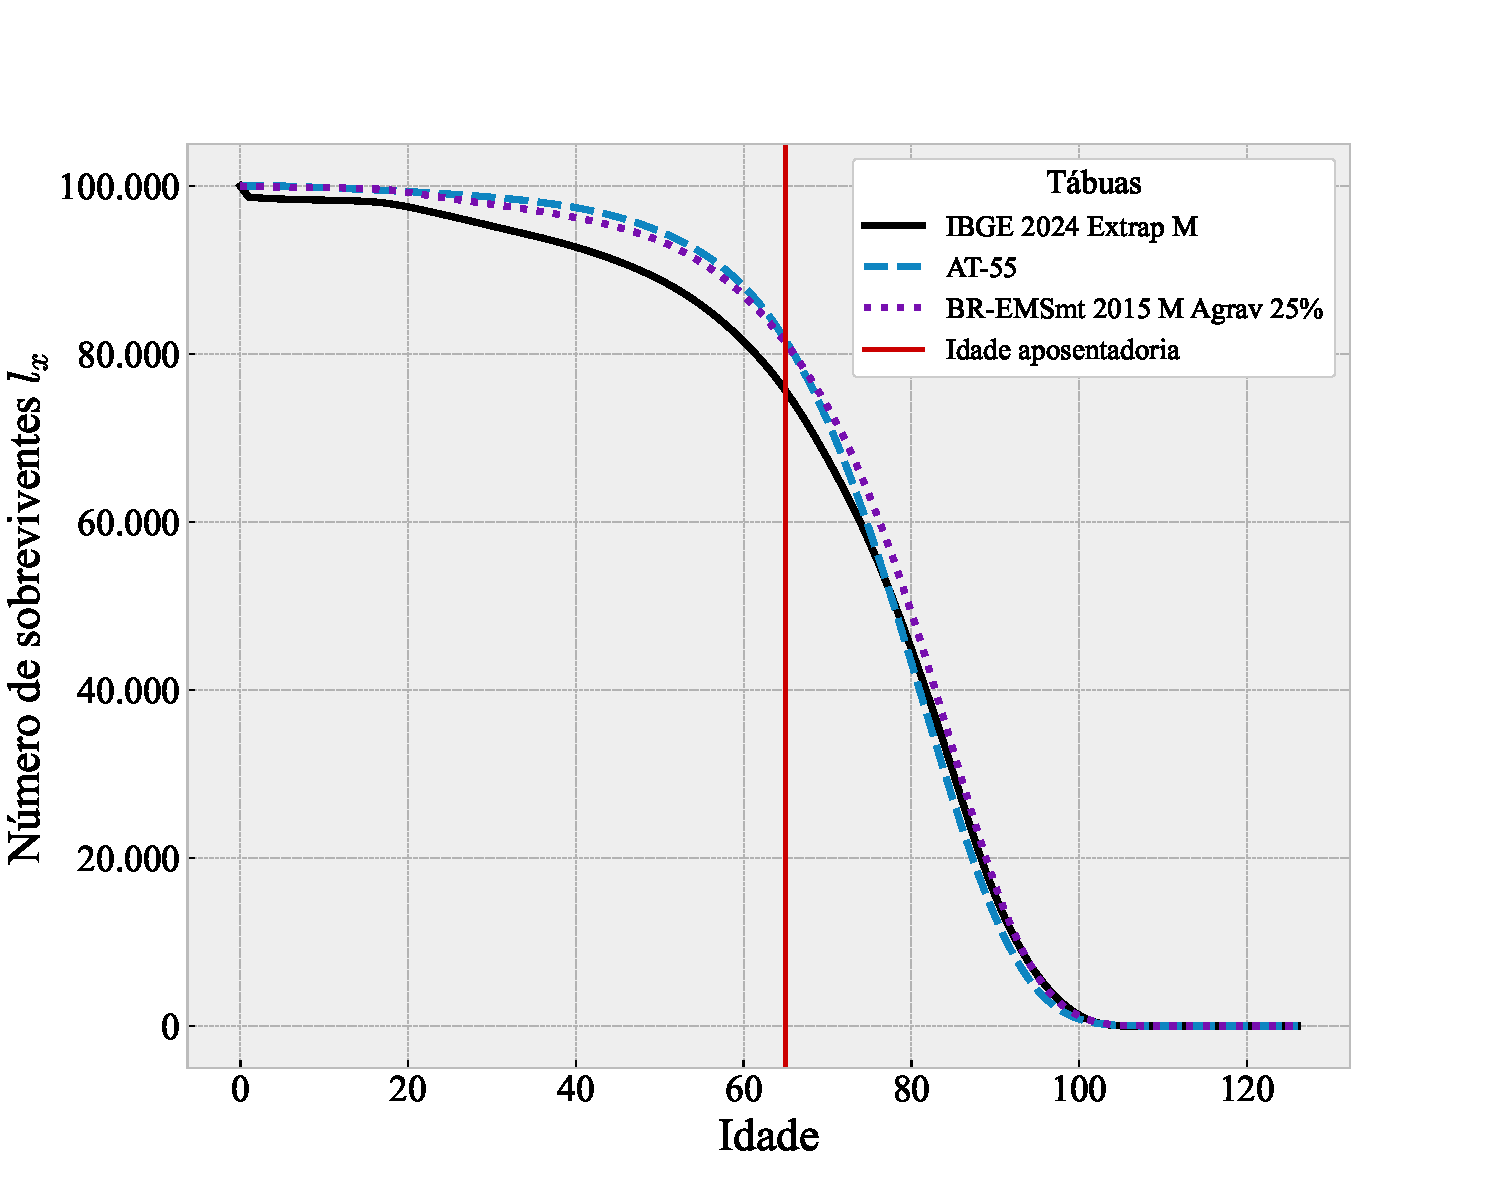
\includegraphics[width=0.84\textwidth, trim=0 0 0 2cm, clip]{curva_lx_masc.pdf}
    \fonte{Elaboração própria (2026).}
    \label{fig:curva_lx_jovem_masc}
\end{figure}

A partir da análise visual da Figura \ref{fig:curva_lx_jovem_masc}, observa-se que tanto a tábua AT-55 quanto a tábua BR-EMSmt 2015 Masculina agravada em 25\% apresentam curvas de $l_x$ semelhantes ao longo de todo o período contributivo. Nesse intervalo de idades, ambas permanecem estritamente acima da curva $l_x$ da tábua IBGE 2024 Extrapolada Masculina, o que indica níveis de sobrevivência mais elevados durante a fase contributiva. 

Consequentemente, espera-se que essas tábuas produzam um VACF superior ao obtido com a tábua de referência. Entretanto, após a idade de 65 anos, observa-se uma mudança no comportamento dessas curvas. A partir desse ponto, as curvas passam a se aproximar e eventualmente se cruzam. No caso da tábua AT-55, a curva $l_x$ apresenta uma queda mais acentuada, passando a situar-se abaixo da curva da tábua IBGE 2024 Extrapolada Masculina por volta da idade 75. Já a curva correspondente à tábua BR-EMSmt 2015 Masculina agravada em 25\% apresenta um declínio mais gradual, aproximando-se da curva da tábua de referência apenas por volta da idade 90, mantendo, contudo, sua superioridade.

Esse comportamento sugere implicações distintas para o VABF. No caso da tábua AT-55, a redução mais acentuada da sobrevivência nas idades avançadas indica que o aumento observado no VACF pode não ser acompanhado por um crescimento proporcional no VABF, uma vez que as probabilidades de sobrevivência durante o período de pagamento dos benefícios torna-se relativamente menor. Em contrapartida, para a tábua BR-EMSmt 2015 Masculina agravada em 25\%, o comportamento da curva $l_x$ nas idades mais elevadas é mais próximo ao da tábua de referência. Assim, o aumento do VACF tende a ser acompanhado por um aumento aproximadamente proporcional no VABF.

\begin{figure}[H]
    \centering
    \singlespacing\caption{Curvas $l_x$ Femininas ao Comparar Diferentes Tábuas}
    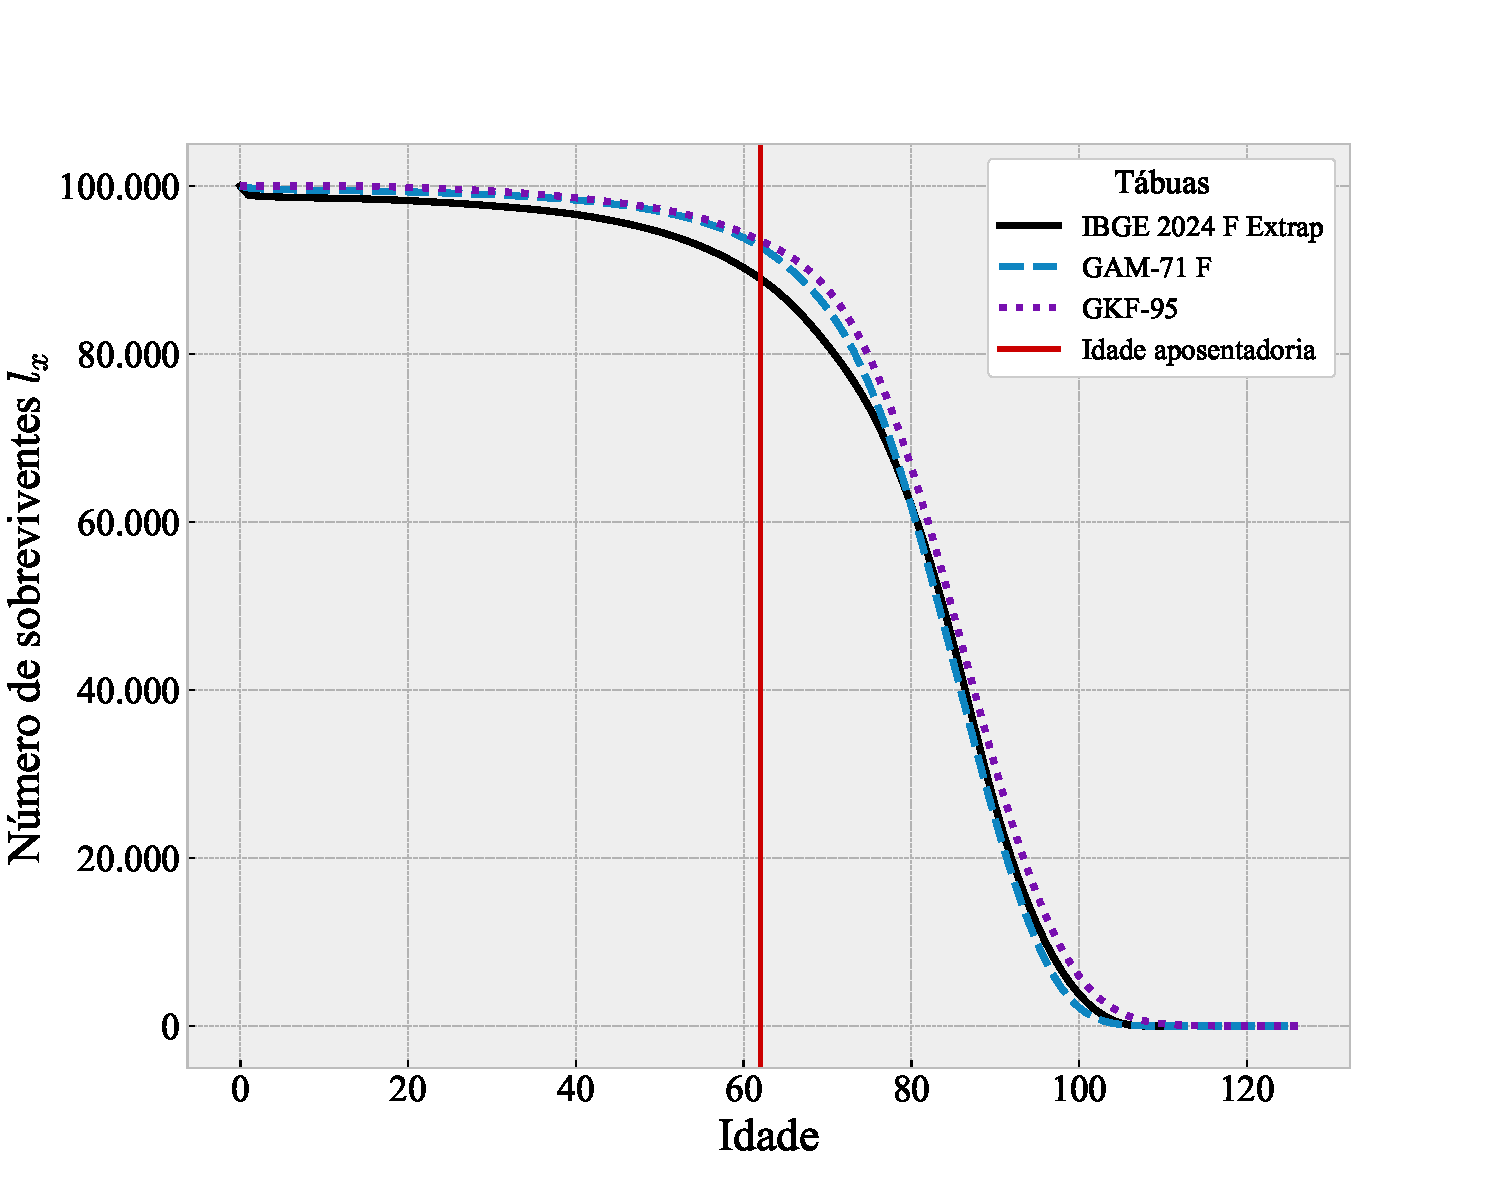
\includegraphics[width=0.84\textwidth, trim=0 0 0 2cm, clip]{curva_lx_fem.pdf}
    \fonte{Elaboração própria (2026).}
    \label{fig:curva_lx_jovem_fem}
\end{figure}

A análise visual da Figura \ref{fig:curva_lx_jovem_fem} apresenta um padrão semelhante ao observado na Figura \ref{fig:curva_lx_jovem_masc}. A tábua GKF-95 mantém sua curva de $l_x$ consistentemente acima da curva da tábua IBGE 2024 Extrapolada Feminina ao longo de todas as idades, aproximando-se da curva da tábua IBGE 2024 Extrapolada Feminina apenas em idade superiores a 85 anos. 

Esse comportamento sugere que o aumento no VACF tende a ser acompanhado por um aumento aproximadamente proporcional no VABF. Por outro lado, a tábua GAM-71 Feminina apresenta um comportamento distinto. Conforme ilustrado na Figura \ref{fig:curva_lx_jovem_fem}, sua curva $l_x$ passa a situar-se abaixo da curva da tábua IBGE 2024 Extrapolada Feminina após os 80 anos. Esse resultado indica que embora possa haver um aumento no VACF durante a fase contributiva, tal aumento não é necessariamente acompanhado por um crescimento proporcional no VABF, devido ao nível relativamente menor de sobrevivência nas idades avançadas.

Portanto, com o índice proposto na Equação \ref{eq:indice}, é possível compreender como os níveis de sobrevivência de $l_x$ são impactados pela distribuição etária da população. Ao calcular os índices referentes aos exemplos de tábuas utilizados na Figura \ref{fig:curva_lx_jovem_masc}, observa-se que a tábua AT-55 apresentou um indicador de aproximadamente $I_{Ativos} = 3,3$ para as idades contributivas, indicando que a tábua comparativa gera um VACF superior àquele obtido pela tábua de referência, o que está em consonância com a discussão realizada na análise visual. 

Essa tábua também apresentou um indicador para as idades de aposentadoria de aproximadamente $I_{Aposentados} = -0,81$, sugerindo que a tábua comparativa gera um VABF inferior ao gerado pela tábua de referência. Por sua vez, a tábua BR-EMSmt 2015 Masculina Agravada em 25\% apresentou indicadores positivos tanto para o período contributivo quanto para o período de aposentadoria, aproximadamente $I_{Ativos} = 2,6$ e $I_{Aposentados}8,6$, respectivamente, indicando que o aumento no VACF foi acompanhado por um aumento no VABF.

Ao analisar os índices calculados para as tábuas GAM-71 e GKF-95, nota-se que os índices da segunda tábua sugerem um VACF maior, acompanhado também de um VABF mais elevado. Nesse caso, os índices observados são de aproximadamente $I_{Ativos} = 1,89$ na fase contributiva e $I_{Aposentados} = 9,04$ nas idades de aposentadoria. Por outro lado, a tábua GAM-71 apresenta um comportamento distinto. O índice de $I_{Ativos} = 1,43$ nas idades contributivas indica que o VACF também é relativamente elevado nessa tábua. Entretanto, nas idades de aposentadoria, o índice observado é de $I_{Aposentados} = 0,61$, sugerindo que o VABF não acompanha, na mesma proporção, o aumento observado no VACF.

As Tabelas \ref{tab:indices_equilibrada_pminf}, \ref{tab:indices_jovem_pminf}, \ref{tab:indices_idosa_pminf} e \ref{tab:indices_bimodal_pminf} apresentam os índices calculados para as fases contributiva e de aposentadoria das tábuas que apresentaram inconsistências nas bases equilibrada, jovem, idosa e bimodal, respectivamente.
\newpage
\begin{table}[htbp]
    \centering
    \caption{Índices da Base Equilibrada para Tábuas com PM Inferior}
    \begin{threeparttable}
    \renewcommand{\arraystretch}{1.0}
    \begin{tabular}{llrr}
    \toprule
    \textbf{Gênero} & \textbf{Tábua} & \textbf{$I_{Ativos}$} & \textbf{$I_{Aposentados}$} \\ 
    \midrule
    \multirow{8}{*}{Masculino} 
        & IBGE 2021 Extrapolada Masculina Suavizada em 1\%      & 0,1860 & -0,2839 \\
        & IBGE 2019 Extrapolada Ambos Agravada em 18,3\%  & 0,8697 &  0,5589 \\
        & AT-2000 Masculina Agravada em 33\%              & 4,0568 &  4,2489 \\
        & AT-55 Suavizada em 5\%                    & 5,5193 &  4,4851 \\
        & AT-83 Basic Masculina Suavizada em 2,5\%          & 6,2039 &  6,3165 \\
        & BR-EMSmt-v.2021 Masculina Agravada em 24\%      & 4,0914 &  4,1542 \\
        & Prudential-50 Suavizada em 16\%           & 5,9100 &  5,0220 \\
        & M-95 H Suavizada em 6\%                   & 1,8742 &  1,2814 \\
    \hline
    \multirow{6}{*}{Feminino}
        & BR-EMSmt-v.2021 Feminina Agravada em 21,5\%    &  1,4900 &  0,8087 \\
        & GAM-71 Feminina Suavizada em 5\%                 &  2,1025 &  4,2357 \\
        & IBGE 2020 Extrapolada Feminina                &  0,2176 & -0,4941 \\
        & IBGE 2019 Extrapolada Ambos Suavizada em 19\% & -1,0670 & -3,3963 \\
        & IBGE 2019 Extrapolada Feminina                &  0,1239 & -1,1209 \\
        & Petros Suavizada em 15\%              &  2,6855 &  2,5947 \\
    \bottomrule
    \end{tabular}
    \begin{tablenotes}[flushleft]
        \small
        \item Fonte: Elaboração própria (2026).
    \end{tablenotes}
    \end{threeparttable}
    \label{tab:indices_equilibrada_pminf}
\end{table}
\vspace{0.5cm}
\begin{table}[htbp]
    \centering
    \caption{Índices da Base Jovem para Tábuas com PM Inferior}
    \begin{threeparttable}
    \renewcommand{\arraystretch}{1.0}
    \begin{tabular}{llrr}
    \toprule
    \textbf{Gênero} & \textbf{Tábua} & \textbf{$I_{Ativos}$} & \textbf{$I_{Aposentados}$} \\ 
    \midrule
    \multirow{12}{*}{Masculino} 
        & IBGE 2019 Extrapolada Ambos Agravada em 19\% & 0,3090 & 0,0375 \\
        & IBGE 2019 Extrapolada Ambos Agravada em 18,3\% & 0,3487 & 0,7004 \\
        & AT-2000 Masculina Agravada em 33\% & 2,1921 & 1,7122 \\
        & AT-55 & 3,3531 & -0,8167 \\
        & AT-55 Suavizada em 5\% & 3,4374 & 2,9086 \\
        & AT-83 Basic Masculina & 3,7035 & 1,6655 \\
        & AT-83 Basic Masculina Suavizada em 2,5\% & 3,7371 & 3,4338 \\
        & BR-EMSmt-v.2021 Masculina Agravada em 24\% & 2,5995 & 2,4447 \\
        & GKM-95 & 2,7029 & -2,4822 \\
        & Prudential-50 Suavizada em 16\% & 3,8411 & 5,0979 \\
        & TR 2025 & 1,6324 & 4,3454 \\
        & M-95 H Suavizada em 6\% & 0,5308 & -0,8540 \\
    \hline
    \multirow{4}{*}{Feminino}
        & BR-EMSmt-v.2021 Feminina Agravada em 21,5\% & 1,2519 & 1,0326 \\
        & GAM-71 Feminina & 1,4372 & 0,6113 \\
        & GAM-71 Feminina Suavizada em 5\% & 1,5006 & 3,1142 \\
        & Petros Suavizada em 13\% & 2,1174 & 0,7493 \\
    \bottomrule
    \end{tabular}
    \begin{tablenotes}[flushleft]
        \small
        \item Fonte: Elaboração própria (2026).
    \end{tablenotes}
    \end{threeparttable}
    \label{tab:indices_jovem_pminf}
\end{table}

\FloatBarrier
A partir da Tabelas \ref{tab:indices_equilibrada_pminf} e \ref{tab:indices_jovem_pminf} observa-se que parte das tábuas inconsistentes segue o padrão verificado nos exemplos anteriores, isto é, $I_{Ativo} > I_{Aposentado}$. Entretanto, também se identificam tábuas inconsistentes que não seguem esse comportamento. Nesses casos, verifica-se $I_{Aposentados} > I_{Ativos}$, ainda assim resultando em uma PM inferior àquela obtida com a tábua de referência, o que evidencia uma limitação do índice proposto. 
\newpage
Tal limitação pode estar associada à complexidade inerente ao cálculo da PM, bem como a determinadas particularidades dos métodos de custeio. Como o índice proposto avalia apenas a tábua de mortalidade, ele não capta a influência das demais premissas atuariais que compõem o cálculo da PM, tampouco do mecanismo de determinação das contribuições. Um exemplo é o método PNI, no qual a premissa de crescimento salarial influencia diretamente o valor das contribuições.
\vspace{0.25cm}
\begin{table}[htbp]
    \centering
    \caption{Índices da Base Idosa para Tábuas com PM Inferior}
    \begin{threeparttable}
    \renewcommand{\arraystretch}{1.0}
    \begin{tabular}{llrr}
    \toprule
    \textbf{Gênero} & \textbf{Tábua} & \textbf{$I_{Ativos}$} & \textbf{$I_{Aposentados}$} \\ 
    \midrule
    \multirow{5}{*}{Masculino} 
        & Prudential-50 Suavizada em 19\% & 6,6859 & 7,6000 \\
        & RP-2000 M               & 9,6269 & 21,665 \\
        & UP - 94 M	               & 8,3839 & 15,369 \\
        & TR 2025                  & 1,9063 & 4,1501 \\
        & Petros                   & 9,6252 & 24,157 \\ \hline
    \multirow{4}{*}{Feminino}
        & AT-83 Basic F  & 3,8171 & 8,8050 \\
        & RP-2000 F  & 3,7881 & 6,2794 \\
        & CL5	 & 3,2476 & 10,7634 \\
        & M-95 M Suavizada em 7\%  & 1,1250 & 1,7197 \\
    \bottomrule
    \end{tabular}
    \begin{tablenotes}[flushleft]
        \small
        \item Fonte: Elaboração própria (2026).
    \end{tablenotes}
    \end{threeparttable}
    \label{tab:indices_idosa_pminf}
\end{table}

No contexto da base idosa, apenas duas tábuas, uma por gênero, produziram PM inferior à da referência nos métodos de custeio INE e PUC. Estas tábuas apresentam $I_{Aposentados} > I_{Ativo} > 0$, indicando que a sobrevivência é superior à da referência em todo o intervalo de idades, com destaque para as idades avançadas. Entretanto, para esse perfil etário com massa de ativos reduzida, mesmo um índice contributivo modesto pode representar um crescimento do VACF suficiente para, em conjunto com o crescimento do VABF, resultar em PM menor. O mecanismo opera, portanto, não pela dominância do VACF sobre o VABF, mas pelo equilíbrio proporcional entre os dois componentes dentro de uma estrutura com poucos ativos.

As demais tábuas apresentadas na Tabela \ref{tab:indices_idosa_pminf} — Prudential-50 Suav. 19\%, TRP-2000 M, UP-94 M, Petros (masculino) e AT-83 Basic F, RP-2000 F, CL5 (feminino) — apresentam índices consideravelmente mais elevados, especialmente no que diz respeito ao $I_{Aposentados}$. Entretanto, essa tábuas só apresentam inconsistências no método de custeio PNI e, portanto, como discutido nos resultados da Tabela \ref{tab:indices_jovem_pminf}, o indicador proposto não é afetado pela premissa de crescimento salarial utilizada no cálculo do VACF nesse método de custeio.

\newpage
\begin{table}[htbp]
    \centering
    \caption{Índices da Base Bimodal para Tábuas com PM Inferior}
    \begin{threeparttable}
    \renewcommand{\arraystretch}{1.0}
    \begin{tabular}{llrr}
    \toprule
    \textbf{Gênero} & \textbf{Tábua} & \textbf{$I_{Ativos}$} & \textbf{$I_{Aposentados}$} \\ 
    \midrule
    \multirow{5}{*}{Masculino} 
        & IBGE 2019 Extrapolada Ambos Agravada em 18,3\% & 0,8839 & 0,8056 \\
        & Prudential-50 Suavizada em 18\%         & 6,5978 & 6,8022 \\
        & RP-2000 M                        & 9,6270 & 21,6652 \\
        & UP - 94 M                        & 8,3840 & 15,3693 \\
        & Petros                           & 9,6252 & 24,1574 \\ \hline
    \multirow{3}{*}{Feminino}
        & AT-83 Basic Feminina      & 3,8171 & 8,8050 \\
        & GAM-71 Feminina Suavizada em 5\%  & 2,9656 & 3,8695 \\
        & RP-2000 Feminina          & 3,7882 & 6,2795 \\
    \bottomrule
    \end{tabular}
    \begin{tablenotes}[flushleft]
        \small
        \item Fonte: Elaboração própria (2026).
    \end{tablenotes}
    \end{threeparttable}
    \label{tab:indices_bimodal_pminf}
\end{table}

Para o contexto da base bimodal as tábuas A IBGE 2019 Extrap. A Agravada 18,3\% e GAM-71 Feminina Suav. 5\%  apresentaram resultados inconsistentes nos métodos INE e CUP. Porém, apenas a tábua IBGE 2019 Extrap. A Agravada 18,3\% apresentou o índice de ativos maior que o índice de aposentados. A GAM-71 Feminina Suav. 5\% apresentou $I_{Aposentados} > I_{Ativos}$, nesse caso, o diferencial de sobrevivência nas idades avançadas não é suficientemente elevado para que o VABF supere o crescimento do VACF impulsionado pelos ativos jovens, resultando em PM inferior nos métodos INE e CUP. Já as tábuas Prudential-50 Suav. 18\%, RP-2000 M, UP-94 M, Petros, AT-83 Basic F e RP-2000 F só apresentam inconsistências no método de custeio PNI, tendo as mesma justificativa das demais tábuas que apresentaram inconsistências nesses método, como com $I_{Aposentados} > I_{Ativos}$.

A Tabela \ref{tab:inconsistencias_br_ems} exemplifica como o mecanismo de suavização/agravamento pode resultar em uma tábua com PM inferior mesmo com expectativa de vida na idade média superior, por meio do indicador proposto, utilizando a tábua BR-EMSmt-v.2021 masculina na base jovem.
\vspace{0.25cm}
\begin{table}[htbp]
    \centering
    \caption{Tábuas com inconsistência observada}
    \begin{threeparttable}
    \renewcommand{\arraystretch}{1.2}
    \begin{tabular}{lrrcc}
    \toprule
    \textbf{Tábua} & $I_{Ativos}$ & $I_{Aposentados}$ \\ \midrule
    BR-EMSmt-v.2021 Masculina & 3,183085 & 22,579169 \\
    BR-EMSmt-v.2021 Masculina Agravada em 10\% & 2,977077 & 14,823639 \\
    BR-EMSmt-v.2021 Masculina Agravada em 15\% & 2,856231 & 10,622265 \\
    BR-EMSmt-v.2021 Masculina Agravada em 20\% & 2,720576 & 6,181995 \\
    BR-EMSmt-v.2021 Masculina Agravada em 24\% & 2,599464 & 2,444722 \\ 
    \bottomrule
    \end{tabular}
    \begin{tablenotes}[flushleft]
        \small
        \item Fonte: Elaboração própria (2026).
    \end{tablenotes}
    \end{threeparttable}
    \label{tab:inconsistencias_br_ems}
\end{table}

A leitura dos índices revela que à medida que o fator de agravamento aumenta de $0\%$ a $24\%$, o $I_{Ativos}$ decresce de forma relativamente contida, de $3,18$ para $2,60$, ao passo que o $I_{Aposentados}$ colapsa de $22,58$ para $2,44$, uma queda de cerca de $89\%$. Essa divergência na taxa de redução dos dois índices é o mecanismo central da inconsistência.

Na tábua sem agravamento, o $I_{Aposentados}$ é aproximadamente sete vezes superior ao $I_{Ativos}$, indicando que o diferencial de sobrevivência da tábua comparativa em relação à referência é substancialmente mais pronunciado nas idades de aposentadoria do que nas idades contributivas. Nesse cenário, o aumento do VABF supera amplamente o aumento do VACF, de modo que a PM resultante é superior à da tábua de referência.

Entretanto, o agravamento progressivo da tábua atua de forma desigual sobre as duas fases do ciclo previdenciário. A mortalidade adicional introduzida pelo fator de agravamento reduz a sobrevivência em todas as idades, mas seu efeito é proporcionalmente muito mais severo nas idades avançadas. Em contrapartida, nas idades contributivas, a diferença entre as curvas $l_x$ da tábua comparativa e da referência é estruturalmente menor, de modo que o agravamento tenha a mesma intensidade. O resultado é que, a cada incremento do fator de agravamento, o $I_{Aposentados}$ encolhe muito mais rapidamente do que o $I_{Ativos}$. Esse exemplo ilustra, portanto, que a inconsistência, isto é, a PM inferior, não é uma propriedade intrínseca da tábua em sua forma original, mas pode ser induzida pelo próprio processo de calibração.

Em resumo, essa seção identificou situações em que tábuas comparativas com expectativa de vida na idade média superior à da tábua de referência produzem PM inferiores. Os resultados revelam uma relação inversa entre a idade média da massa e a frequência dessas inconsistências. Isto é, as bases mais jovens concentraram os maiores números de ocorrências, enquanto as bases mais idosas registram poucos casos. Esse padrão é atribuído ao fato de que, em massas predominantemente contributivas, o excesso de sobrevivência das tábuas comparativas nas idades ativas eleva o VACF sem contrapartida proporcional no VABF, reduzindo a PM.

O método PNI, dentre os três métodos avaliados, apresentou maior propensão a inconsistências em todas as bases — acumulando 30 ocorrências masculinas e 16 femininas, frente a 19 e 9 do INE —, comportamento associado à premissa de crescimento salarial incorporada ao cálculo do VACF. O sexo masculino concentra mais inconsistências na maioria dos cenários, possivelmente em razão da maior variabilidade histórica da mortalidade masculina. Adicionalmente, o processo de calibração por suavização ou agravamento pode induzir inconsistências inexistentes na tábua original, como demonstrado com a BR-EMSmt-v.2021 M, cujo agravamento progressivo reduz o diferencial de sobrevivência nas idades de benefício de forma muito mais acentuada do que nas idades contributivas.

Para explicar o tais resultados, esta seção propõe dois índices — $I_{Ativos}$ e $I_{Aposentados}$ — que mensuram o diferencial acumulado de sobrevivência entre a tábua comparativa e a de referência em cada fase do ciclo previdenciário. Em geral, inconsistências ocorrem quando $I_{Ativos} > I_{Aposentados}$, embora casos com o padrão inverso também sejam identificados, o que evidencia uma limitação do índice. Por considerar apenas a tábua de mortalidade, ele não captura a influência das demais premissas atuariais.

% !TEX root = tcc.tex
\chapter{\textbf{CONSIDERAÇÕES FINAIS}}

Este capítulo consolida as principais conclusões do estudo, discute suas limitações e aponta direções para pesquisas futuras que possam vir a cobrir as lacunas deixadas pela presente pesquisa.

O presente trabalho investigou o impacto da aplicação do critério de validação de tábuas de mortalidade estabelecido pelo Art. 36, inciso I, da Portaria MTP nº 1.467/2022, sobre as PM dos RPPS. O critério em questão determina que, caso o ente não use a tábua de referência, a tábua adotada deve apresentar, na idade média da massa segurada, uma expectativa de vida igual ou superior àquela calculada pela tábua de referência. Em todos os quatro perfis etários analisados foram identificadas tábuas de mortalidade que atenderam ao critério normativo, isto é, apresentaram expectativa de vida na idade média superior à da tábua de referência, mas que, ao mesmo tempo, produziram uma PM inferior àquela gerada pela tábua de referência (IBGE 2024 Extrapolada para cada gênero).

As tábuas que apresentaram uma PM inferior variaram conforme o perfil etário e o método de custeio adotado. Com relação ao perfil etário, as simulações indicam que massas seguradas com estrutura etária mais jovem, especialmente a do sexo masculino, podem ser mais suscetíveis à ocorrência de inconsistências. Na base jovem, onde aproximadamente 60\% dos segurados concentram-se na faixa de 18 a 30 anos, os métodos INE e CUP identificaram dez e oito inconsistências para o sexo masculino, respectivamente, além de três para o sexo feminino em cada um desses métodos. O método de custeio PNI, por sua vez, apresentou o maior número total de inconsistências em todos os perfis, somando 16 ocorrências na base jovem, sendo 12 para o sexo masculino e 4 para o sexo feminino. A base equilibrada mostrou um comportamento semelhante a base jovem, embora tenha apresentando um numero menor de inconsistências.

Em contrapartida, a base idosa, com concentração majoritária de segurados acima dos 51 anos e idade média de 65,13 anos, apresentou o menor número de inconsistências nos métodos INE e CUP, registrando apenas uma tábua inconsistente para cada sexo. A base bimodal comportou-se de maneira semelhante à base idosa nesses dois métodos, em razão do elevado peso relativo dos grupos de aposentados.

A investigação do comportamento da curva de $l_x$ indicou que a assimetria entre os níveis de sobrevivência nas tábuas pode ser o motivo de tais inconsistências. Uma tábua comparativa pode apresentar níveis de sobrevivência superiores à tábua de referência ao longo das idades contributivas $[18, 64]$, o que eleva o VACF, e simultaneamente apresentar níveis de sobrevivência inferiores nas idades de aposentadoria $[65, \omega]$, reduzindo o VABF. Tal assimetria explica o aumento da expectativa de vida na tábua comparativa, além de implicar na variação do VACF superando a variação no VABF, resultando em uma PM inferior à da tábua de referência, ainda que a expectativa de vida na idade média seja igual ou superior.

Esse mecanismo foi quantificado pelo índice $I_F$ proposto na Equação \ref{eq:indice}, o qual tenta mensurar o diferencial de sobrevivência ponderado pela distribuição etária da massa, separadamente para as faixas contributivas e para as faixas em gozo de benefício. A análise dos índices para as tábuas inconsistentes das bases jovem e equilibrada evidenciou que, em sua maioria, essas tábuas apresentam $I_{Ativos} > I_{Aposentados}$, confirmando o padrão esperado. As exceções observadas, em particular no método PNI, reforçam que o índice proposto, embora útil como instrumento de diagnóstico prévio, não incorpora a complexidade total no cálculo da PM, principalmente no método de custeio PNI.

Adicionalmente, os resultados indicaram uma possível vulnerabilidade normativa específica. O mecanismo de suavização e agravamento de tábuas de mortalidade pode ser utilizado para modelar tábuas que, embora tecnicamente aprovadas pelo critério do Art. 36, produzem PM inferiores às da tábua de referência. Tábuas como a BR-EMSmt-v.2021 M Agravada em 24\% e Prudential-50 Suavizada apareceram de forma consistente em múltiplos perfis e métodos, embora suas versões sem alterações não aparecem. A esse respeito, a pesquisa sugere que é possível suavizar ou agravar uma tábua de mortalidade de tal forma que ela mantenha a expectativa de vida na idade média próxima à da tábua de referência, satisfazendo o critério normativo, mas resultando em uma PM inferior.

Em síntese, o estudo indica que o critério de validação estabelecido pelo Art. 36 da Portaria MTP nº 1.467/2022, ao utilizar a expectativa de vida na idade média como único parâmetro de comparação, pode ser insuficiente para garantir, em todas as configurações demográficas possíveis, que a tábua adotada pelo RPPS resulte em uma provisão matemática igual ou superior àquela gerada pela tábua do IBGE.

Embora os resultados obtidos sejam consistentes, algumas limitações devem ser consideradas na interpretação deste trabalho. A primeira limitação diz respeito ao uso exclusivo de dados simulados. A construção de bases populacionais sintéticas, embora seja fundamental para isolar o efeito da estrutura etária sobre o passivo atuarial em condições controladas, impede a extrapolação direta dos resultados quantitativos para RPPS específicos. As magnitudes das inconsistências identificadas, bem como o número exato de tábuas inconsistentes por perfil, são sensíveis às configurações das massas simuladas e às premissas adotadas. A aplicação da metodologia a bases reais de RPPS poderia revelar padrões distintos em termos de intensidade e frequência das inconsistências.

A segunda limitação está relacionada à simplificação das variáveis consideradas na análise. Para evidenciar com maior clareza o impacto das tábuas de mortalidade sobre a PM, o estudo restringiu-se ao benefício de aposentadoria por idade, desconsiderando outros decrementos relevantes no contexto previdenciário, como a invalidez e a reversão de pensão, por exemplo. Da mesma forma, adotou-se valor único de remuneração inicial ($R\$~5.000,00$) para todos os segurados, abstraindo a heterogeneidade salarial presente nas massas reais dos RPPS. Essas simplificações, ao reduzirem a complexidade do modelo, podem subestimar ou superestimar o efeito das inconsistências em cenários mais aderentes à realidade.

Por fim, o índice $I_F$ proposto, embora útil como instrumento de diagnóstico e interpretação das inconsistências, não incorpora explicitamente o efeito do crescimento salarial sobre o VACF no método PNI. Isso implica que o índice, em sua forma atual, possui menor poder preditivo para inconsistências nesse método específico, representando uma limitação da ferramenta diagnóstica desenvolvida neste trabalho.

Uma primeira direção natural consiste na replicação da metodologia aqui desenvolvida com dados reais de RPPS. A aplicação do índice $I_F$ a bases reais permitiria avaliar a prevalência das inconsistências identificadas nas simulações no contexto factual dos regimes brasileiros, além de verificar se determinados perfis demográficos observados na prática são mais expostos ao problema normativo descrito.

Uma segunda linha de pesquisa poderia estender o modelo atuarial para incorporar múltiplos decrementos, contemplando invalidez, desligamento e pensão por morte. A inclusão dessas variáveis tornaria o modelo mais próximo da realidade dos RPPS e permitiria avaliar se o fenômeno das inconsistências se mantém ou se atenua quando a interação entre diferentes riscos biométricos é considerada.

Em terceiro lugar, seria relevante investigar a sensibilidade das inconsistências em relação às premissas econômicas, particularmente à taxa de juros e à taxa de crescimento salarial. Análises de cenários com diferentes trajetórias dessas variáveis contribuiriam para mapear as condições sob as quais as inconsistências são mais ou menos graves.

Outra perspectiva é o aprimoramento do índice $I_F$, de modo a incorporar a complexidade do cálculo da PM em cada método de custeio. Um índice estendido que contemplasse, simultaneamente, os diferenciais de sobrevivência, de crescimento salarial e de outras premissas atuariais, apresentaria maior poder preditivo, tornando-se uma ferramenta robusta para o diagnóstico prévio de inconsistências.

Do ponto de vista regulatório, estudos futuros poderiam propor e testar critérios alternativos ou complementares ao estabelecido no Art. 36 da Portaria MTP nº 1.467/2022. Entre as possibilidades, sugerem-se critérios baseados em métricas distribucionais das tábuas de mortalidade como percentis ponderados pela estrutura etária da massa. Tal critério poderia ser mais robustos a assimetrias demográficas do que a comparação pontual de expectativas de vida.

Por fim, pesquisas que examinem o comportamento de tábuas geracionais no contexto do Art. 36 representam uma extensão importante. As tábuas geracionais incorporam a perspectiva de melhoria contínua da mortalidade ao longo do tempo e são reconhecidas na literatura como mais adequadas para a mensuração do risco de longevidade em planos de longo prazo. A investigação de como o critério normativo se comporta diante dessas tábuas, especialmente em massas jovens, poderia revelar novas dimensões do problema identificado neste estudo.


% ===== REFERÊNCIAS =====
\newpage
\renewcommand{\bibname}{REFERÊNCIAS}
\bibliographystyle{abntex2-alf}
\bibliography{referencias} 
\addcontentsline{toc}{chapter}{REFERÊNCIAS}


% ===== APÊNDICES =====

% !TEX root = tcc.tex
\newpage
\appendix 

% 1. Cria a âncora para o link do sumário funcionar corretamente
\phantomsection 

% 2. Adiciona ao sumário (agora o link apontará para cá)
\addcontentsline{toc}{chapter}{APÊNDICE A - CONTRAEXEMPLOS PARA A RELAÇÃO ENTRE EXPECTATIVA DE VIDA E ANUIDADES}

% 3. Título centralizado
\begin{center}
    APÊNDICE A - CONTRAEXEMPLOS PARA A RELAÇÃO ENTRE EXPECTATIVA DE VIDA E ANUIDADES
\end{center}

% 4. Faz o label 'pegar' o valor A e não o número do capítulo anterior
\renewcommand{\thechapter}{Apêndice A}
\refstepcounter{chapter}
\label{apendice_A}

% 5. Configuração das equações
\counterwithin{equation}{chapter}
\setcounter{equation}{0}
\renewcommand{\theequation}{A.\arabic{equation}}

Seja $PM^{i}_{x}$ a provisao matemática de um segurado de idade $x$, calculada a partir da tábua de mortalidade $i$. Logo, sejam $e^{*}_{\overline{X}}$  expectativa de vida na idade média segundo uma tábua comparativa qualquer e $PM^{*}_{x}$ provisão matemática correspondente, sendo $e^{\kappa}_{\overline{X}}$ a expectativa de vida na idade média segundo a tábua de referência e $PM^{\kappa}_{x}$ a respectiva provisão matemática.

Para analisar a implicação $e^{*}_{x} \geq e^{\kappa}_{x} \Rightarrow PM^{*}_{x} \geq PM^{\kappa}_{x}$ é necessário entender, primeramente, a relação matemática entre $e_{x}$ e as anuidades atuariais, dado que a provisão $PM$ depende explicitamente dos valores da anuidades atuariais que a compõem. Tomando, como exemplo, a anuidade atuarial vitalicia postecipada $a_{x}$, tem-se que:

\begin{equation}
    e_{x} = \sum_{t=1}^{\omega - x} {}_{t}p_x
    \label{apB:ex}
\end{equation}

\begin{equation}
    a_{x} = \sum_{t=1}^{\omega - x} v^t \cdot {}_{t}p_x
    \label{apB:ax}
\end{equation}

As equações \ref{apB:ex} e \ref{apB:ax} possuem uma representação em termos de álgebra linear. Para tanto, primeiro é necessário definir os vetores coluna de dimensão $t = \omega - x$ no espaço $\mathbb{R}^k$:

\begin{equation}
    \mathbf{p}_x = 
    \begin{bmatrix} 
    {}_{1}p_x \\  
    {}_{2}p_x \\ 
    \vdots \\ 
    {}_{t}p_x 
    \end{bmatrix}, \quad 
    \mathbf{v} = 
    \begin{bmatrix} 
    v^1 \\ 
    v^2 \\ 
    \vdots \\ 
    v^t 
    \end{bmatrix}, \quad 
    \mathbf{1} = 
    \begin{bmatrix} 
    1 \\ 
    1 \\ 
    \vdots \\ 
    1 
    \end{bmatrix}
\end{equation}

Dessa forma, as equações \ref{apB:ex} e \ref{apB:ax} podem ser expressas como produtos escalares facilitando a visualiação algébrica da seguinte forma:

\begin{equation}
    e_{x} = \mathbf{1}^\top \mathbf{p}_x
    \label{apB:exvetor}
\end{equation}

\begin{equation}
    a_{x} = \mathbf{v}^\top \mathbf{p}_x
    \label{apB:axvetor}
\end{equation}

As formulas \ref{apB:exvetor} e \ref{apB:axvetor} evidênciam que única diferença entre a expectativa de vida e a anuidade atuarial é o vetor de juros. Isso corrobora com a intuição de se $e_x$ é maior, então $a_x$ também será e consequemente, a provisão matemática também será.
\newpage
Supondo vetores de probabilidade de tamanho $t=3$, sejam $p^{*}=(p^{*}_{0}, p^{*}_{1}, p^{*}_{2})$ e $p^{\kappa}=(p^{\kappa}_{0}, p^{\kappa}_{1}, p^{\kappa}_{2})$ correspondentes às tábuas comparativa e referência, respectivamente. Tem-se que:

\begin{equation}
    e^{*}_x \geq e^{\kappa}_{x}
\end{equation}
\begin{equation}
    {}_{1}p^{*}_x + {}_{2}p^{*}_x + {}_{3}p^{*}_x \geq {}_{1}p^{\kappa}_x + {}_{2}p^{\kappa}_x + {}_{3}p^{\kappa}_x
    \label{apB:desi1}
\end{equation}
Então é esperado que,
\begin{equation}
    a^{*}_x \geq a^{\kappa}_{x}
\end{equation}
\begin{equation}
    {}_{1}p^{*}_x v + {}_{2}p^{*}_x v^{2} + {}_{3}p^{*}_x v^{3} \geq {}_{1}p^{\kappa}_x v + {}_{2}p^{\kappa}_x v^{2} + {}_{3}p^{\kappa}_x v^{3}
\end{equation}
\begin{equation}
    {}_{1}p^{*}_x  + {}_{2}p^{*}_x  v + {}_{3}p^{*}_x  v^2 \geq {}_{1}p^{\kappa}_x  + {}_{2}p^{3}_x  v + {}_{3}p^{\kappa}_x  v^2
    \label{apB:desi2}
\end{equation}

Definindo as difernças $d_i = {}_{i}p^{*}_x - {}_{i}p^{\kappa}_x$ e com ${}_{i}p^{*}_x,{}_{i}p^{\kappa}_x \in [0,1]$, logo $d_i \in [-1, 1]$, então as desigualdades \ref{apB:desi1} e \ref{apB:desi2} tornam-se nas desiguladaes \ref{apB:dif_ex} e \ref{apB:dif_ax}, respectivamente.

\begin{equation}
    D_1 = d_0 + d_1 + d_2 \geq 0
    \label{apB:dif_ex}
\end{equation}
\begin{equation}
    D_2 = d_0 + d_1v + d_2v^2 \geq 0
    \label{apB:dif_ax}
\end{equation}

Onde a desigualdade \ref{apB:dif_ex} é uma soma simples, enquanto a desigualdade \ref{apB:ax} é uma soma ponderada com coeficientes decrescentes. Para que a implicação $e^{*}_x \geq e^{\kappa}_x \Rightarrow a^{*}_x \geq a^{\kappa}_x$ seja falsa, é necessário que \ref{apB:dif_ex} seja verdadeira mas \ref{apB:dif_ax} falsa. Isto é, é necessário que $D_1 \geq 0$ e $D_2 < 0$. Isso ocorre quando $d_1$ é negativa, gerando a desigualdade dupla na expressão \ref{apB:cond_geral}.

\begin{equation}
    d_1 + d_2 + d_3 \geq 0 \Rightarrow d_2 + d_3 \geq -d_1
\end{equation}
\begin{equation}
    d_1 + d_2v + d_3v^2 < 0 \Rightarrow d_2v + d_3v^2 < -d_1 
\end{equation}

Ou seja, para que ambas inequações sejam verdadeiras, é necessário que:

\begin{equation}
    d_2v + d_3v^2 < -d_1 \leq d_2 + d_3
    \label{apB:cond_geral}
\end{equation}

Como $v<1$, a condição da inequação dupla \ref{apB:cond_geral} é satisfeita quando as probabilidades iniciais na tábua de referência são maiores que as da tábua comparativa, ou seja, ${}_{1}p^{\kappa}_x > {}_{1}p^{*}_x$. Se ${}_{1}p^{\kappa}_x > {}_{1}p^{*}_x$, então $d_1$ é negativo, permitindo que a condição  (esperança de vida maior ou igual) seja mantida por compensações nos termos $d_2$ e $d_3$, enquanto $D_2<0$ (anuidade menor) ocorre porque o fator $v<1$ reduz o impacto dessas compensações futuras no valor presente.

Além deste contra-exemplo algebrico, é possível, a partir de simulações computacionais, desenvolver um algoritmo que forneça um contra-exemplo numérico com valores mais realistas, como mostra a Figura \ref{fig:pseudocodigo_numerico}.

\begin{figure}[H]
    \singlespacing\caption{Pseudocódigo Contra-exemplo Numérico}
    \begin{algorithm}[H]
        \caption{Geração de Contra-exemplos Numérico}
        \label{alg:contraexemplo}
        \begin{algorithmic}[1]
        \STATE \textbf{Parâmetros:}
        \STATE $v \gets \frac{1}{1+i}$ \hfill $\triangleright$ Fator de desconto
        \STATE $n \gets 100.000$ \hfill $\triangleright$ Número de tentativas
        \STATE $s$ \hfill $\triangleright$ Semente reprodutória
        \STATE \textbf{Inicialização:}
        \STATE $\text{solucoes} \gets [\,]$ \hfill $\triangleright$ Lista vazia para armazenar resultados
        \FOR{$i = 1$ \textbf{até} $n$}
            \STATE \textbf{Gerar} ${}_{1}p^{*}_x, {}_{2}p^{*}_x, {}_{3}p^{*}_x, {}_{1}p^{\kappa}_x, {}_{2}p^{\kappa}_x, {}_{3}p^{\kappa}_x \sim U(0,1)$ \hfill $\triangleright$ Números aleatórios entre 0 e 1
            \STATE \textbf{Verificar Condições:}
            \STATE $\text{cond}_1 \gets ({}_{1}p^{*}_x + {}_{2}p^{*}_x + {}_{3}p^{*}_x) \geq ({}_{1}p^{\kappa}_x + {}_{2}p^{\kappa}_x + {}_{3}p^{\kappa}_x)$ \hfill $\triangleright$ Condição sobre $e_x$
            \STATE $\text{cond}_2 \gets ({}_{1}p^{*}_x + v {}_{2}p^{*}_x + v^2 {}_{3}p^{*}_x) < ({}_{1}p^{\kappa}_x + v {}_{2}p^{\kappa}_x + v^2 {}_{3}p^{\kappa}_x)$ \hfill $\triangleright$ Condição sobre $a_x$
            \STATE $\text{cond}_3 \gets {}_{1}p^{*}_x > {}_{2}p^{*}_x > {}_{3}p^{*}_x$ \hfill $\triangleright$ Decrescimento em $*$
            \STATE $\text{cond}_4 \gets {}_{1}p^{\kappa}_x > {}_{2}p^{\kappa}_x > {}_{3}p^{\kappa}_x$ \hfill $\triangleright$ Decrescimento em $r$
            \IF{$\text{cond}_1 \land \text{cond}_2 \land \text{cond}_3 \land \text{cond}_4$}
                \STATE $\text{solucoes.adicionar}(({}_{1}p^{*}_x, {}_{2}p^{*}_x, {}_{3}p^{*}_x, {}_{1}p^{\kappa}_x, {}_{2}p^{\kappa}_x, {}_{3}p^{\kappa}_x))$
            \ENDIF
        \ENDFOR
        \RETURN $\text{solucoes[0]}$ \hfill $\triangleright$ Retorna a primeira solução
        \end{algorithmic}
    \end{algorithm}
    \fonte{Elaboração própria (2026).}
    \label{fig:pseudocodigo_numerico}
\end{figure}

Com uma taxa de juros anual de 5\%, por exemplo, o algoritmo \ref{alg:contraexemplo} retorná os valores que satizfazem a condição de $e^{*}_{x} \geq e^{\kappa}_{x}$, porém resultam em $a^{*}_{x} < a^{\kappa}_{x}$. São eles: ${}_{1}p^{*}_x = 0,6447, {}_{2}p^{*}_x = 0,5600, {}_{3}p^{*}_x = 0,1214, {}_{1}p^{\kappa}_x = 0,8915, {}_{2}p^{\kappa}_x = 0,4187, {}_{3}p^{\kappa}_x = 0,0104$. Esse valores resultam em $e^{*}_{x} = 1,3261$, $e^{\kappa}_{x} = 1,3205$, porém, $a^{*}_{x} = 1,2882$ e $a^{\kappa}_{x} = 1,2996$. Ou seja, a condição $e^{*}_{x} \geq e^{\kappa}_{x}$, para esses valores, não implicou em $a^{*}_{x} \geq a^{\kappa}_{x}$.


% !TEX root = tcc.tex
\newpage

% 1. Cria a âncora para o link do sumário funcionar corretamente
\phantomsection 

% 2. Adiciona ao sumário (agora o link apontará para cá)
\addcontentsline{toc}{chapter}{APÊNDICE B - DERIVAÇÃO DA FUNÇÃO DE SOBREVIVÊNCIA E DA EXPECTATIVA DE VIDA}

% 3. Título centralizado
\begin{center}
    APÊNDICE B - DERIVAÇÃO DA FUNÇÃO DE SOBREVIVÊNCIA E DA EXPECTATIVA DE VIDA
\end{center}

% 4. Faz o label 'pegar' o valor A e não o número do capítulo anterior
\renewcommand{\thechapter}{Apêndice B}  % atualiza ANTES de capturar
\refstepcounter{chapter}
\label{apendice_B}

% 5. Configuração das equações
\counterwithin{equation}{chapter}
\setcounter{equation}{0}
\renewcommand{\theequation}{B.\arabic{equation}}


É possível escrever a probabilidade de sobrevivência entre as idades $x$ e $x+1$ em função apenas da força de mortalidade. O primeiro passo é escrever \ref{eq:fx} em termos de \ref{eq:Sx}.
\begin{equation}
    f_x(t)=\frac{d}{dt}F_x(t)=\frac{d}{dt}[1-S_x(t)]=-\frac{d}{dt}S_x(t)
    \label{eq:A-fx_Sx}
\end{equation}
Logo, ao substituir \ref{eq:A-fx_Sx} em \ref{eq:mux}, temos apenas força de mortalidade e função de sobrevivência na equação, como mostra \ref{eq:A-muxsx}:
\begin{equation}
    \mu_{x+t} = \frac{-\frac{d}{dt}S_x(t)}{S_x(t)}=\frac{1}{S_x(t)}\cdot\frac{d}{dt}S_x(t)
    \label{eq:A-muxsx}
\end{equation}
Pela regra da cadeia, pode-se rescrever \ref{eq:A-muxsx} de outra forma, como mostra a equação \ref{eq:A-muxsx2}.
\begin{equation}
    \mu_{x+t} = -\frac{d}{dt}lnS_x(t)
    \label{eq:A-muxsx2}
\end{equation}
Integrando ambos os lados da equação \ref{eq:A-muxsx2} em relação a $t$, obtem-se:
\begin{equation}
    \int_0^s\mu_{x+t}dt=-\int_0^s\frac{d}{dt}ln(S_x(t))dt
    \label{eq:A-intmu1}
\end{equation}
\begin{equation}
    \int_0^s\mu_{x+t}dt=-[ln(S_x(s))-ln(S_x(0))]
    \label{eq:A-intmu2}
\end{equation}
A função de sobrevivência no tempo  $t=0$ é 1, isto é, a probabilidade de uma pessoa de idade $x$ viver $0$ anos é $100\%$. Portando, ao aplicar essa propriedade em \ref{eq:A-intmu2}, temos o $ln(1)=0$, o que resulta na equação \ref{eq:A-intmu3}.
\begin{equation}
    \int_0^s\mu_{x+t}dt=-ln(S_x(s))
    \label{eq:A-intmu3}
\end{equation}
Aplicando exponencial de ambos os lados da equação \ref{eq:A-intmu3} e reindexando, obtêm-se a função de sobrevivência em termos da força de mortalidade, como mostra \ref{eq:A-sxmu}.
\begin{equation}
    {}_tp_x=S_x(t)=e^{-\int_0^t\mu_{x+u}du} 
    \label{eq:A-sxmu}
\end{equation}

A partir da definição de uma esperença matemática de um V.A., obtém-se a formula para a expectativa de vida, como mostra a equação \ref{eq:exdifini} \cite{bowers2006}.
\begin{equation}
    e_x^0=\int_0^\infty t \cdot  f_x(t)dt = \int_0^\infty t \cdot {}_{t}p_x \cdot \mu_{x+t} dt 
    \label{eq:exdifini}
\end{equation}

Ao derivar a equação \ref{eq:A-sxmu} é possível encontrar um termo semelhante a função densidade $f_x(t) = {}_{t}p_x \cdot \mu_{x+t}$ da equação \ref{eq:exdifini}. Para derivar a equação \ref{eq:A-sxmu}, aplica-se a regra da cadeia. Primeiro, tomando o logaritmo natural em ambos os lados da equação:
\begin{equation}
    {}_tp_x=e^{-\int_0^t\mu_{x+u}du}
\end{equation}
\begin{equation}
    ln({}_tp_x)=-\int_0^t\mu_{x+u}du
\end{equation}
\begin{equation}
    \frac{d}{dt}ln({}_tp_x)=-\int_0^t\mu_{x+u}du
    \label{eq:ddt}
\end{equation}

O teorema fundamental do cálculo estabelece que, se $f$ for contínua em um intervalo e definimos $F(t) = \int_{a}^{t}f(u)du$, então $F'=f(t)$. Ou seja, a derivada de uma integral em relação ao limite superior é o valor do integrando naquele limite. Portanto, o lado direito da equação \ref{eq:ddt} torna-se:
\begin{equation}
    G(t) = \int_0^t\mu_{x+u}du
\end{equation}
\begin{equation}
    G'(t) = \mu_{x+t}
\end{equation}
Logo,
\begin{equation}
    \frac{d}{dt} \left(-\int_0^t\mu_{x+u}du\right) = -G'(t) = -\mu_{x+t}
    \label{eq:mufinal}
\end{equation}

Para o lado esquerdo da equação \ref{eq:ddt}, usando efetivamente a regra da cadeia, obtem-se a equação \ref{eq:ddtpx}:
\begin{equation}
    \frac{d}{dt}ln({}_tp_x) = \frac{1}{{}_tp_x} \cdot \frac{d}{dt}({}_tp_x)
    \label{eq:ddtpx}
\end{equation}
Subustituindo os resultados obtidos em \ref{eq:mufinal} e \ref{eq:ddtpx} na equação \ref{eq:ddt}:
\begin{equation}
    \frac{1}{{}_tp_x} \cdot \frac{d}{dt}({}_tp_x) = -\mu_{x+t}
    \label{eq:pxfinales}
\end{equation}
Multiplicando ambos os lados por $-{}_{t}p_{x}$
\begin{equation}
    -\frac{d}{dt}({}_tp_x) = {}_tp_x \cdot \mu_{x+t}
    \label{eq:finales}
\end{equation}

Dessa forma, com a expressão obtida equação \ref{eq:finales} é possível reescrever a equação \ref{eq:exdifini} da seguinte forma:
\begin{equation}
    e_{x}^{0} = \int_{0}^{\infty} t \cdot \left( -\frac{d}{dt}({}_tp_x) \right)dt = -\int_{0}^{\infty} t \cdot \left(\frac{d}{dt}({}_tp_x) \right)dt
    \label{finales3}
\end{equation}

Para resolver \ref{finales3} é necessário usar o método de integração por partes. Seja $u=t$ e $dv=\left(\frac{d}{dt}({}_tp_x) \right)$, então:
\begin{equation}
    e_{x}^{0} = -\int_{0}^{\infty} t \cdot \left(\frac{d}{dt}({}_tp_x) \right)dt = -\left(\left[t \cdot {}_{t}p_x \right]_{0}^{\infty} - \int_0^{\infty} {}_{t}p_xdt\right)
\end{equation}
\begin{equation}
    e_{x}^{0} = -\left[t \cdot {}_{t}p_x \right]_{0}^{\infty} + \int_0^{\infty} {}_{t}p_x dt
\end{equation}

Em $t=0$, tem-se que $t\cdot {}_{t}p_x = 0 \cdot {}_{0}p_x = 0$. Em $t \to \infty$ é necessário analisar o que acontece com $t \cdot {}_{t}p_x$ quando $t$ tende ao infinito. Ou seja, avaliar $lim_{t \to \infty} t \cdot {}_{t}p_x$. Dado que ${}_{t}p_x$ é uma probabilidade de sobrevivência, esse produto tende a 0, devido a propriedade das probabilidades de sobrevivência \cite{dickson2019}. Portanto, $e_x^{0}$ se torna apenas:

\begin{equation}
    e_{x}^{0} = \int_0^{\infty} {}_{t}p_x dt
    \label{eq:exfinal100}
\end{equation}

% !TEX root = tcc.tex
\newpage
\phantomsection 
\addcontentsline{toc}{chapter}{APÊNDICE C - TÁBUAS DE MORTALIDADE E CÓDIGOS}
\begin{center}
    APÊNDICE C - TÁBUAS DE MORTALIDADE E CÓDIGOS
\end{center}
\renewcommand{\thechapter}{Apêndice C}
\refstepcounter{chapter}
\label{apendice_C}
\counterwithin{equation}{chapter}
\setcounter{equation}{0}
\renewcommand{\theequation}{C.\arabic{equation}}

Todos os códigos elaborados para execução deste trabalho podem ser encontrados no repositório GitHub: \url{https://github.com/st3nd1/TCC}.

Todas as tábuas de mortalidade usadas para o cálculo da PM nesse estudo podem ser encontradas na Tabela \ref{tab:tabuas_utilizadas}. Com exceção das tábuas TR-2025 \cite{ssa_actuarial_life_table}, Petros \cite{soa_petros_2822}, M-95 H \cite{soa_m95h_23001}, M-95 F \cite{soa_m95m_23002}, todas as tábuas podem ser encontradas no endereço eletronico: \url{https://atuarios.org.br/tabuas-biometricas/} \cite{iba_tabuas_biometricas}.

\begin{singlespace}
\begin{longtable}{clcl}
\caption{Tábuas de Mortalidade Masculinas e Femininas Utilizadas nas Provisões Matemáticas}
\label{tab:tabuas_utilizadas} \\
\toprule
\multicolumn{1}{c}{\textbf{N°}} & \multicolumn{1}{c}{\textbf{Tábua Masculina}} & \multicolumn{1}{c}{\textbf{N°}} & \multicolumn{1}{c}{\textbf{Tábua Feminina}} \\
\midrule
\endfirsthead
\multicolumn{4}{c}{\small\textit{(continuação)}} \\
\toprule
\multicolumn{1}{c}{\textbf{N°}} & \multicolumn{1}{c}{\textbf{Tábua Masculina}} & \multicolumn{1}{c}{\textbf{N°}} & \multicolumn{1}{c}{\textbf{Tábua Feminina}} \\
\midrule
\endhead
\midrule
\multicolumn{4}{r}{\small\textit{(continua)}} \\
\endfoot
\bottomrule
\multicolumn{4}{l}{\small Fonte: Elaboração própria (2026).} \\
\endlastfoot
1  & IBGE 2024 Extrap M                & 1  & IBGE 2024 F Extrap \\
2  & IBGE 2023 M                       & 2  & IBGE 2023 F \\
3  & IBGE 2023 Extrap M                & 3  & IBGE 2023 A \\
4  & IBGE 2022 M                       & 4  & IBGE 2020 Extrap. F \\
5  & IBGE 2022 Extrap M                & 5  & IBGE 2019 Extrap. Ambos \\
6  & IBGE 2022 Extrap M Suav 7,5\%    & 6  & IBGE 2019 Extrap. Ambos Suave 19\% \\
7  & IBGE 2021 M                       & 7  & IBGE 2019 Extrap. F \\
8  & IBGE 2021 Extrap M                & 8  & IBGE 2018 Extrap. A \\
9  & IBGE 2021 Extrap M Suav 1\%      & 9  & IBGE 2018 Extrap. F \\
10 & IBGE 2020 Extrap. M               & 10 & AT-2000 (Suav 10\%) F \\
11 & IBGE 2019 Extrap. A               & 11 & AT-2000 F \\
12 & IBGE 2019 Extrap. A Agrav 19\%   & 12 & AT-49 F \\
13 & IBGE 2019 Extrap. A Agrav 18,3\% & 13 & AT-50 \\
14 & IBGE 2019 Extrap. M               & 14 & AT-55 \\
15 & IBGE 2018 Extrap. A               & 15 & AT-83 Basic F \\
16 & IBGE 2018 Extrap. M               & 16 & AT-83 IAM F \\
17 & IBGE 2018 Extrap. M Suave 2,5\%  & 17 & BR-EMSmt-v.2021 F \\
18 & AT-2000 (Suav 10\%) M            & 18 & BR-EMSmt-v.2021 F Agrav. 21,5\% \\
19 & AT-2000 M                         & 19 & BR-EMSsb-v.2021 F \\
20 & AT-2000 M Agrav. 33\%            & 20 & BREMSmt 2015 F \\
21 & AT-49 M                           & 21 & BREMSsb 2015 F \\
22 & AT-50                             & 22 & CDG-60 \\
23 & AT-55                             & 23 & GAM-71 F \\
24 & AT-55 Suave 5\%                  & 24 & GAM-71 F Suav 5\% \\
25 & AT-83 Basic M                     & 25 & GAM-71 F Suav 7,5\% \\
26 & AT-83 Basic M Suave 2,5\%        & 26 & GAM-71 F Suav 10\% \\
27 & AT-83 IAM M                       & 27 & CSO80 \\
28 & BR-EMSmt-v.2021 M                & 28 & GKF-95 \\
29 & BR-EMSmt-v.2021 M Agrav 10\%    & 29 & GR-95 F \\
30 & BR-EMSmt-v.2021 M Agrav 15\%    & 30 & Prudential-50 \\
31 & BR-EMSmt-v.2021 M Agrav 20\%    & 31 & AMERICAN EXPERIENCE \\
32 & BR-EMSmt-v.2021 M Agrav 24\%    & 32 & RP-2000 F \\
33 & BR-EMSmt 2015 M                  & 33 & SGB-51 \\
34 & BR-EMSmt 2015 M Agrav 20\%      & 34 & SGB-75 \\
35 & BR-EMSmt 2015 M Agrav 25\%      & 35 & Rentiers Francais \\
36 & BREMSsb 2015 M                   & 36 & UP - 94 F \\
37 & CDG-60                            & 37 & USTP - 61 \\
38 & GAM-71 M                          & 38 & 2012 AIM table F \\
39 & CSO80                             & 39 & CL5 \\
40 & GKM-70                            & 40 & CL6 \\
41 & GKM-95                            & 41 & Hunter Semitropical \\
42 & GR-95 M                           & 42 & Grupal Americana \\
43 & Prudential-50                     & 43 & TR 2025 \\
44 & Prudential-50 Suav. 16\%         & 44 & Petros \\
45 & Prudential-50 Suav. 17\%         & 45 & Petros Suavizada 5\% \\
46 & Prudential-50 Suav. 18\%         & 46 & Petros Suavizada 7,5\% \\
47 & Prudential-50 Suav. 19\%         & 47 & Petros Suavizada 10\% \\
48 & Prudential-50 Suav. 19,5\%       & 48 & Petros Suavizada 13\% \\
49 & Prudential-50 Suav. 20\%         & 49 & Petros Suavizada 15\% \\
50 & AMERICAN EXPERIENCE              & 50 & Petros Suavizada 17\% \\
51 & RP-2000 M                         & 51 & M-95 M \\
52 & SGB-75                            & 52 & M-95 M Suav. 2\% \\
53 & Rentiers Francais                 & 53 & M-95 M Suav. 3\% \\
54 & UP - 94 M                         & 54 & M-95 M Suav. 5\% \\
55 & USTP - 61                         & 55 & M-95 M Suav. 7\% \\
56 & 2012 AIM table M                 & 56 & M-95 M Agravada 10\% \\
57 & CL5                               & & \\
58 & CL6                               & & \\
59 & Hunter Semitropical               & & \\
60 & Grupal Americana                  & & \\
61 & TR 2025                           & & \\
62 & Petros                            & & \\
63 & M-95 H                            & & \\
64 & M-95 H Suave 6\%                 & & \\
\end{longtable}
\end{singlespace}



\end{document}